\chapter{Implementation and Evaluation}
\label{chap:implementation}

\section*{Introduction}

Chapter~\ref{chap:design} described the design and the boundaries between the
deterministic optimizer, the application platform, and the governed agentic layer.
This chapter moves from design to implementation. It first presents the main
technologies used across the platform. It then documents the implemented product
through a screenshot showcase that follows the user journey, from product entry to
result interpretation, and reports the surrounding platform and operations work
(enterprise access, delivery, monitoring, and observability). The evaluation of the
assisted behavior is reported last, before the chapter conclusion.

\section{Main technologies}
\label{sec:tech}

The implementation reused the existing Energy Transition Optimizer foundation and
extended it with a governed agentic layer, a restored platform, and an
observability and evaluation stack. The stack was therefore not a greenfield
choice but a pragmatic combination of the technologies already present in the
product and those required to restore, secure, deploy, and extend it. This section
covers the main technologies only; supporting libraries are treated as
implementation details where they become relevant.

\subsection{Frontend technologies}

\paragraph{Next.js.} Next.js provides the routing, build model, and React-based
foundation behind the product workspace, supporting project navigation, topology
editing, assumption ingestion, simulation review, and the agentic chat interface.
\begin{center}
\includegraphics[height=1.4cm]{Figures/tech/nextjs.png}\end{center}

\paragraph{TypeScript.} TypeScript is the main frontend language; typing the API
contracts, component properties, application state, and generated client models
makes client-side development safer around structured domain objects such as
topologies, approval cards, and streamed agentic events.
\begin{center}
\includegraphics[height=1.4cm]{Figures/tech/typescript.png}\end{center}

\subsection{Backend and deterministic execution}

\paragraph{Python.} Python is the main backend and computation language, shared by
the API service, the deterministic optimization engine, background workers, and the
agentic implementation, which keeps product, solver, and agent logic close to the
same domain model.
\begin{center}
\includegraphics[height=1.4cm]{Figures/tech/python.png}\end{center}

\paragraph{FastAPI.} FastAPI exposes the application API for projects, ingestion,
simulations, agentic sessions, approvals, and health checks, with a typed
request-response model that matters when agentic proposals must be validated before
reaching application state.
\begin{center}
\includegraphics[height=1.4cm]{Figures/tech/fastapi.png}\end{center}

\paragraph{OR-Tools.} OR-Tools is the optimization technology behind the
deterministic core, responsible for the constrained scheduling that produces
operational and financial outputs; the project preserved this deterministic
authority rather than replacing it with language-model reasoning.
\begin{center}
\includegraphics[height=1.4cm]{Figures/tech/ortools.png}\end{center}

\paragraph{Celery.} Celery runs long simulations as asynchronous background work,
so the API stays responsive while deterministic computation runs outside the
request-response path; its workers are treated as a dedicated execution layer.
\begin{center}
\includegraphics[height=1.4cm]{Figures/tech/celery.png}\end{center}

\subsection{Agentic technologies}

\paragraph{LangChain and LangGraph.} LangChain provides the agent and tool-calling
foundation used by the Director, while LangGraph structures specialist workflows as
explicit state graphs, supporting bounded delegation, streaming, resumable state,
and approval-gated interactions rather than an unstructured chatbot.
\begin{center}
\includegraphics[height=1.4cm]{Figures/tech/langchain.png}\end{center}

\paragraph{OpenAI-compatible models.} OpenAI-compatible chat models provide the
reasoning capability of the agentic layer; their authority is intentionally
constrained, since model outputs become structured proposals rather than direct
mutations of project state.
\begin{center}
\includegraphics[height=1.4cm]{Figures/tech/openai.png}\end{center}

\paragraph{Langfuse.} Langfuse is the observability platform for the agentic layer,
recording model calls, tool trajectories, traces, evaluator scores, and prompt
versions so that assisted behavior can be inspected after execution.
\begin{center}
\includegraphics[height=1.4cm]{Figures/tech/langfuse.png}\end{center}

\subsection{Persistence and messaging}

\paragraph{PostgreSQL.} PostgreSQL provides durable checkpointing for the agentic
layer, keeping conversational execution state separate from the core product data
model.
\begin{center}
\includegraphics[height=1.4cm]{Figures/tech/postgresql.png}\end{center}

\paragraph{Redis.} Redis supports queueing and broker availability for asynchronous
execution around the worker path, letting worker scaling depend on the current
broker state rather than a fixed endpoint.
\begin{center}
\includegraphics[height=1.4cm]{Figures/tech/redis.png}\end{center}

\subsection{Cloud, identity, and runtime}

\paragraph{Microsoft Azure.} Azure hosts the deployed environment, including the
Kubernetes cluster, container registry, SQL database, blob storage, networking, and
private access, so the product is treated as a cloud-hosted application rather than
only a local artifact.
\begin{center}
\includegraphics[height=1.4cm]{Figures/tech/azure.png}\end{center}

\paragraph{Terraform.} Terraform is the infrastructure-as-code technology used to
define and restore the environment, and was central to correcting infrastructure
drift and making deployment repeatable.
\begin{center}
\includegraphics[height=1.4cm]{Figures/tech/terraform.png}\end{center}

\paragraph{Docker.} Docker packages application services into container images that
support local development and provide the build artifacts promoted through the
delivery chain.
\begin{center}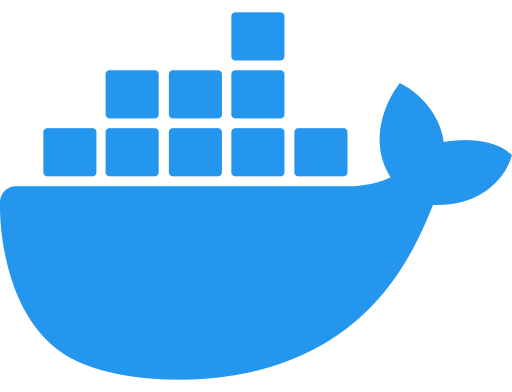
\includegraphics[height=1.4cm]{Figures/tech/docker.png}\end{center}

\paragraph{Kubernetes.} Kubernetes orchestrates the deployed containers, managing
backend replicas, workers, services, secrets, autoscaling, and rollouts.
\begin{center}
\includegraphics[height=1.4cm]{Figures/tech/kubernetes.png}\end{center}

\paragraph{Kagent.} Kagent provides the Kubernetes-native runtime for the read-only
operational QA agent and its inspection tools, enabled with a read-only scope so the
agent observes the platform without becoming an automated remediation actor.
\begin{center}
\includegraphics[height=1.4cm]{Figures/tech/kagent.png}\end{center}

\paragraph{Okta (OpenID Connect).} Okta is the enterprise identity path adopted by
the restored authentication architecture, aligning access control with
organizational identity management and reducing the identity infrastructure the
product operates directly.
\begin{center}
\includegraphics[height=1.4cm]{Figures/tech/okta.png}\end{center}


\paragraph{CircleCI.} CircleCI automates builds and checks; restoring the pipeline
was an early priority, since the product could not be safely renovated or deployed
while delivery depended on manual recovery steps.
\begin{center}
\includegraphics[height=1.4cm]{Figures/tech/circleci.png}\end{center}



\section{Implementation showcase}
\label{sec:journey}

The showcase is organized as a screenshot sequence that follows the implemented
user journey from product entry to deterministic work, agentic assistance,
ingestion, topology generation, and result interpretation. Its purpose is not to
document every interaction, but to demonstrate that the implemented application
covers the full path.

\subsection{Product entry and orientation}

The first screens establish the product framing: they introduce the Energy
Transition Optimizer as an internal decision tool, explain the expected workflow,
and bring the user from a landing page into the project workspace before any data or
simulation is requested (Figures~\ref{fig:impl-landing}
and~\ref{fig:impl-recent}).
This is the visible shift from the inherited, expert-only interface to a reviewable
product surface.

\begin{figure}[H]
  \centering
  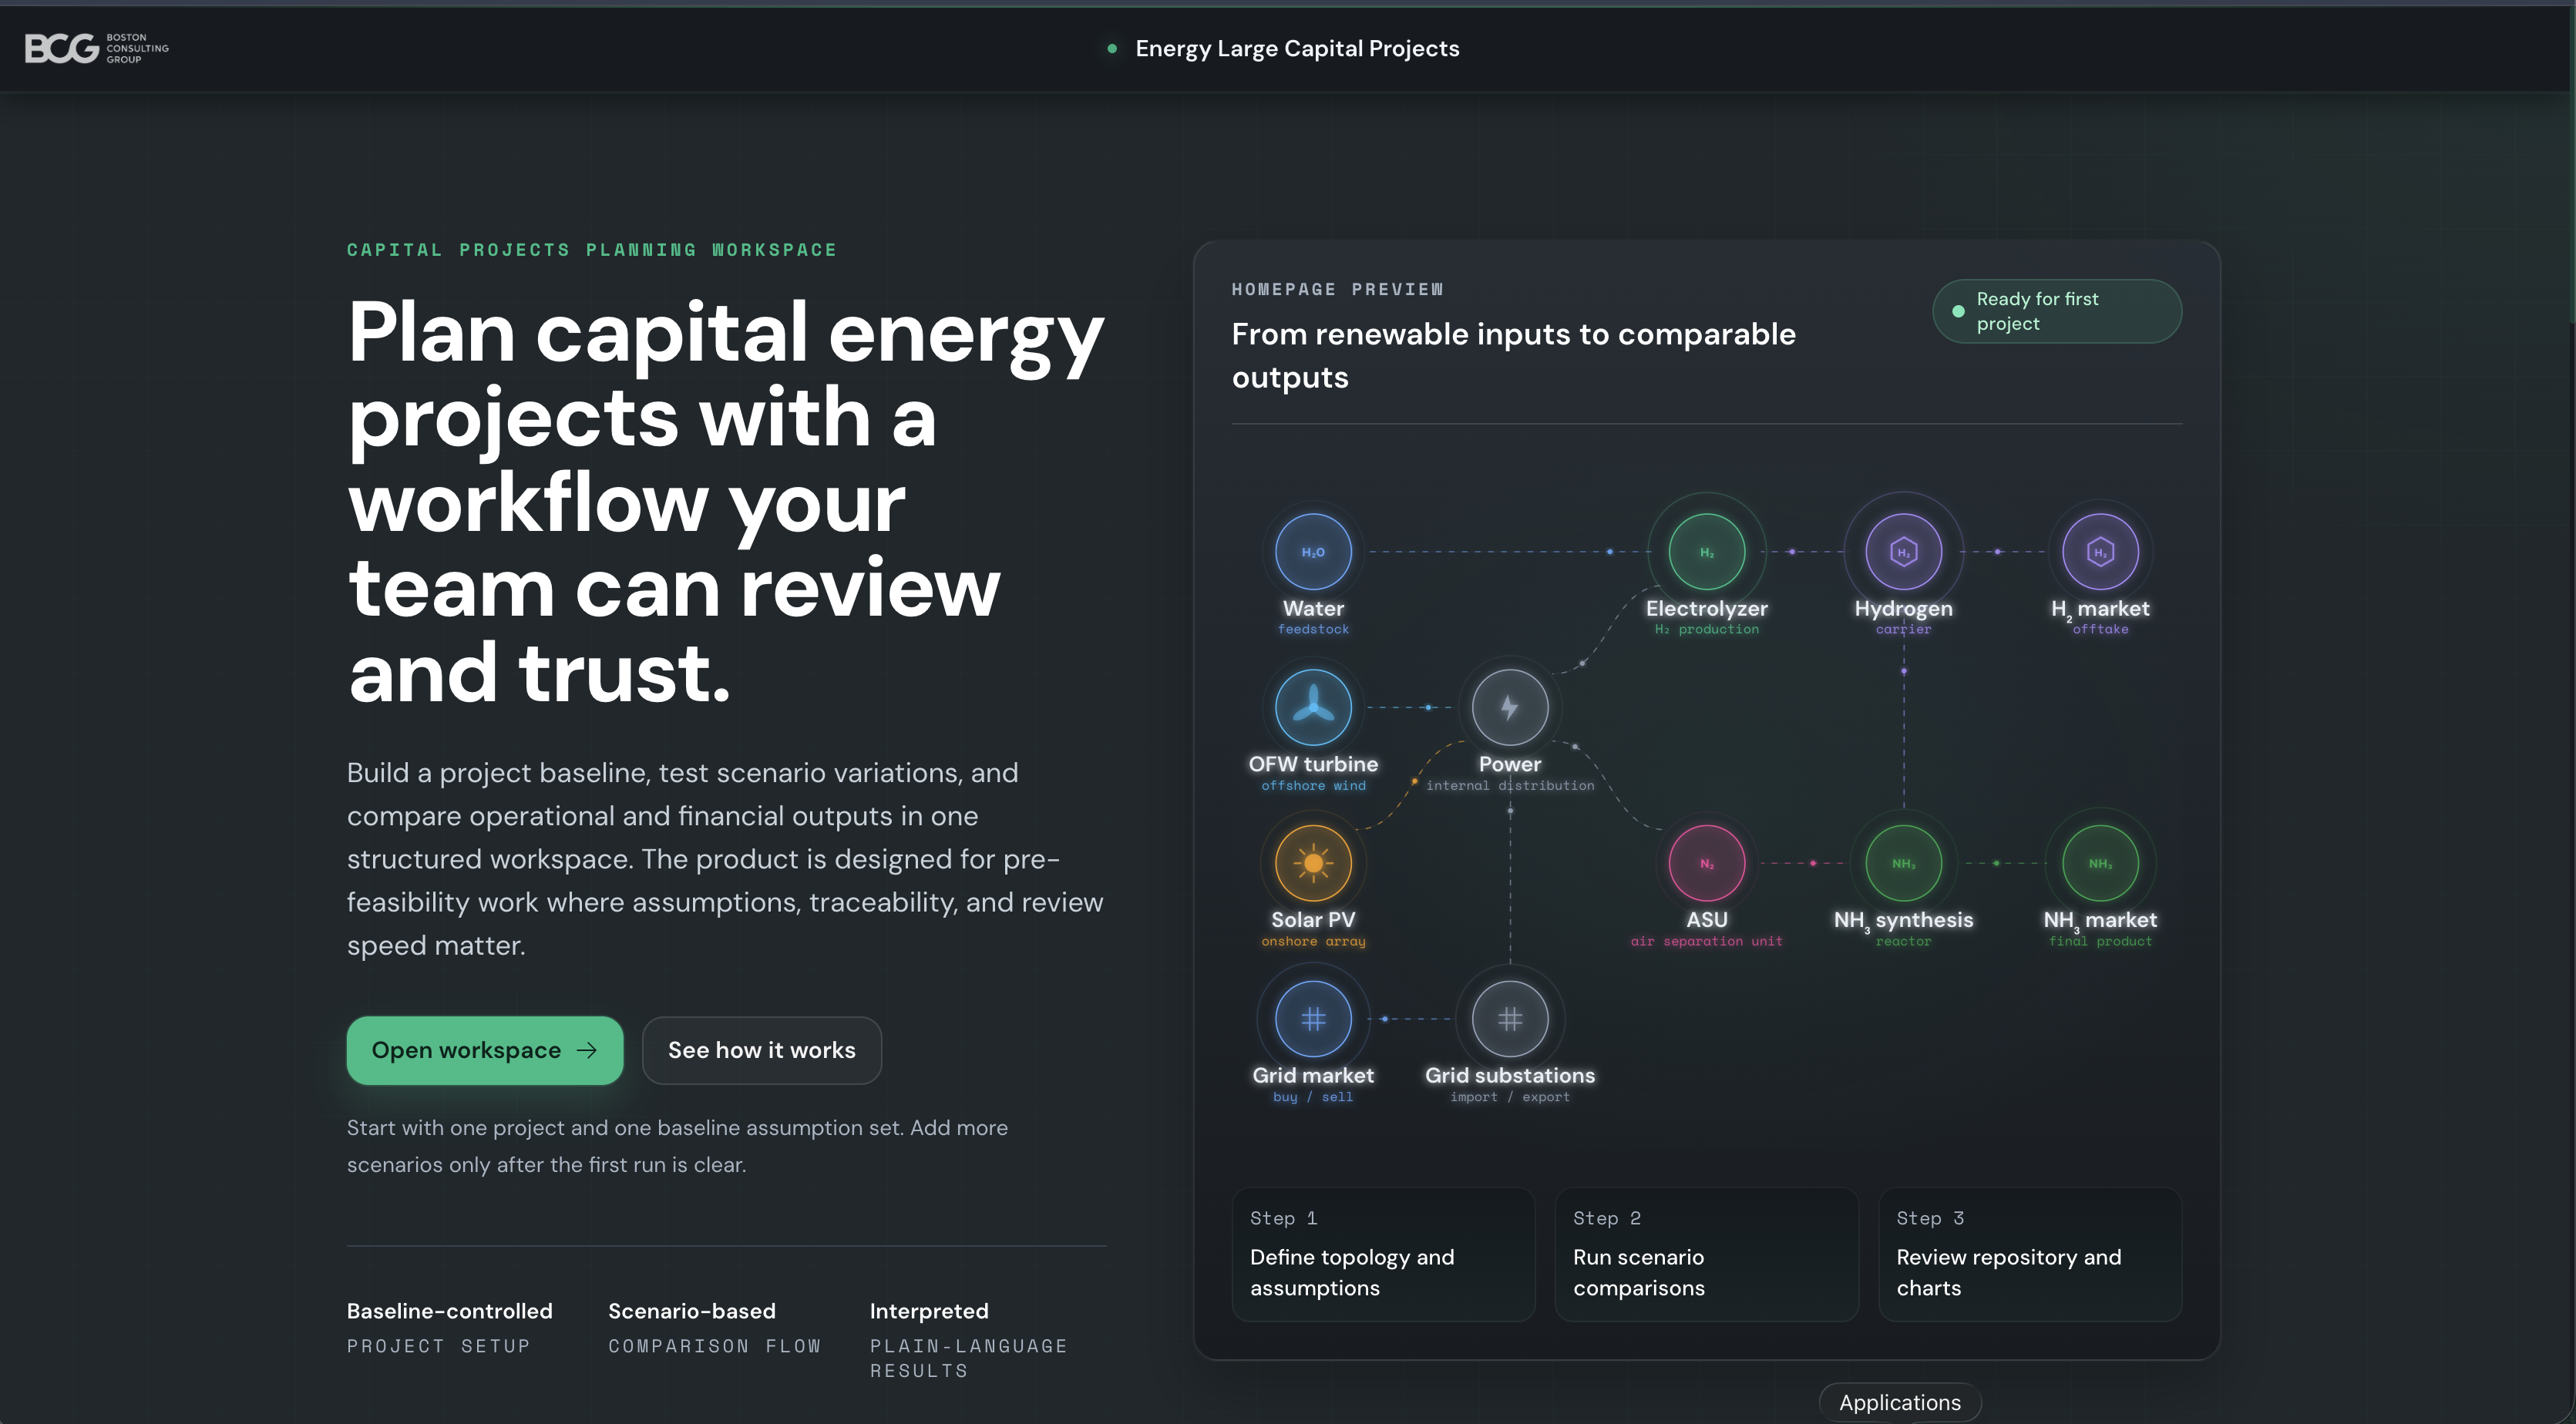
\includegraphics[width=0.95\linewidth]{Figures/chadi_landing.png}
  \caption{Landing page: the optimizer framed as a structured, reviewable workflow.}
  \label{fig:impl-landing}
\end{figure}

\begin{figure}[H]
  \centering
  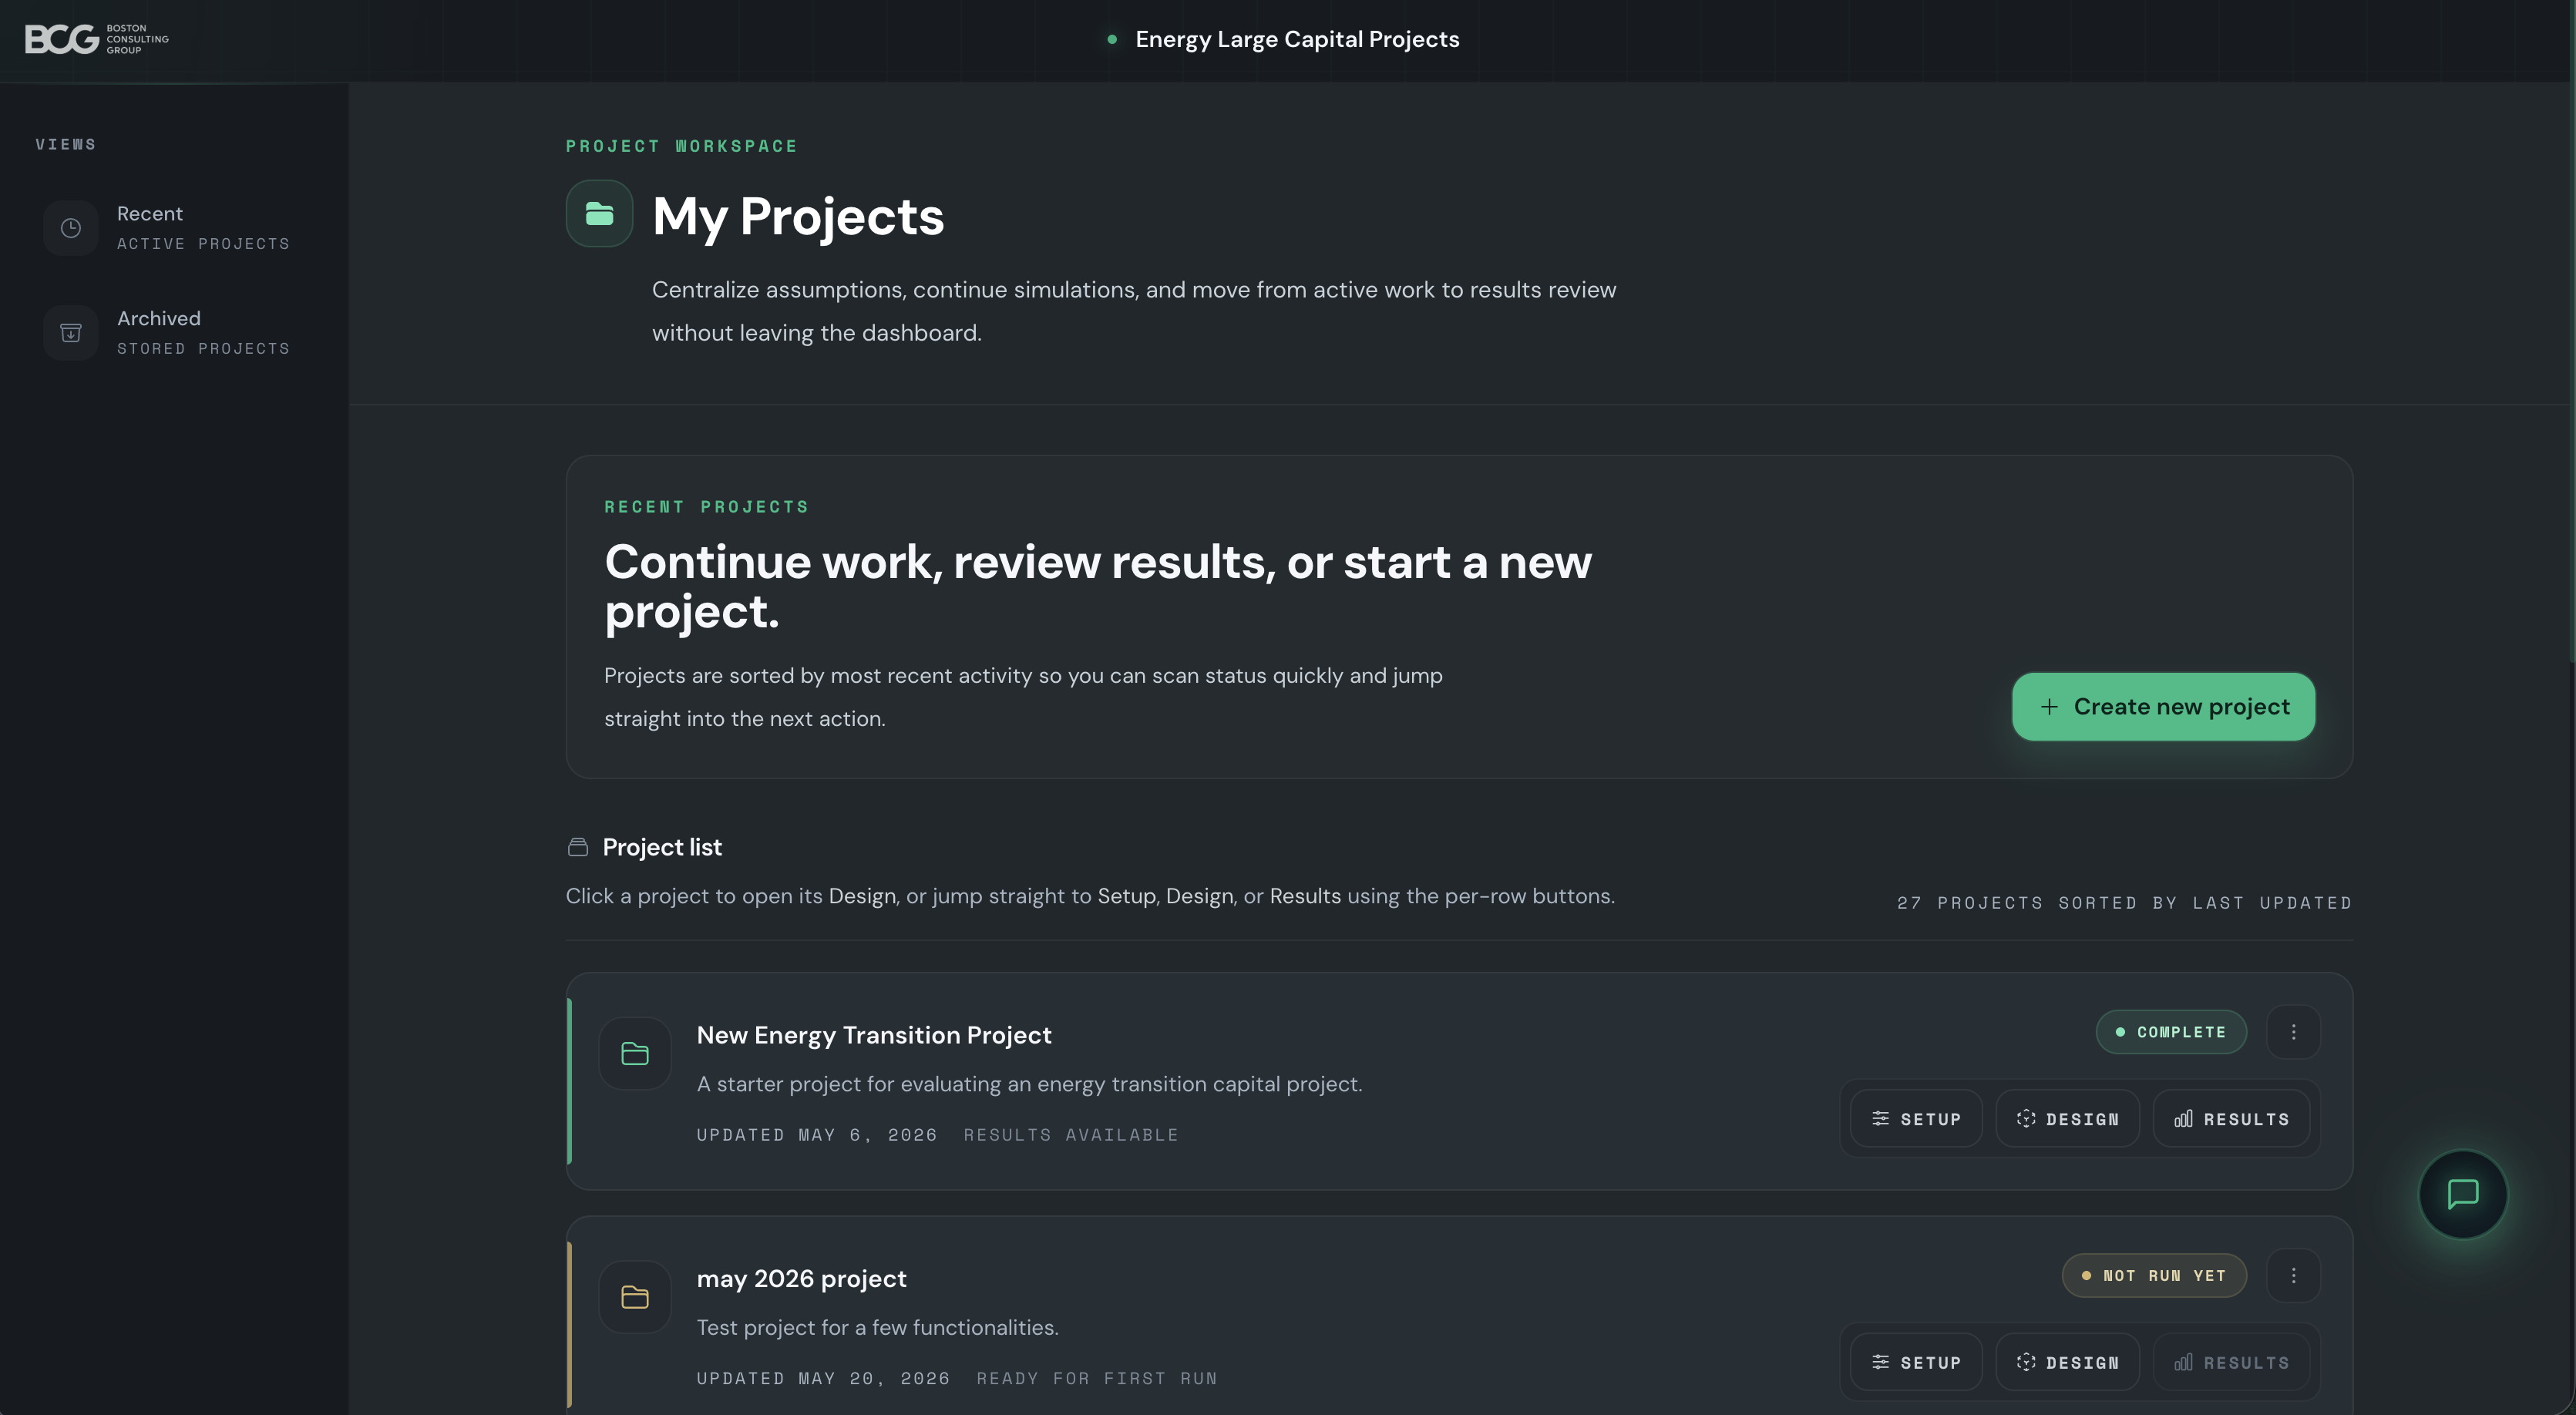
\includegraphics[width=0.95\linewidth]{Figures/chadi_recent_projects.png}
  \caption{Recent projects: continue existing work or start anew from one surface.}
  \label{fig:impl-recent}
\end{figure}

\subsection{Project setup and the deterministic workspace}

The next sequence follows the non-agentic product path: creating a project,
entering assumptions, reviewing and editing the topology, setting parameters and
operating choices, launching simulations, and analyzing deterministic results
(Figures~\ref{fig:impl-data}--\ref{fig:impl-runcharts}). This keeps the
narrative honest: the agentic layer extends a working analytical product, it does
not replace it.

\begin{figure}[H]
  \centering
  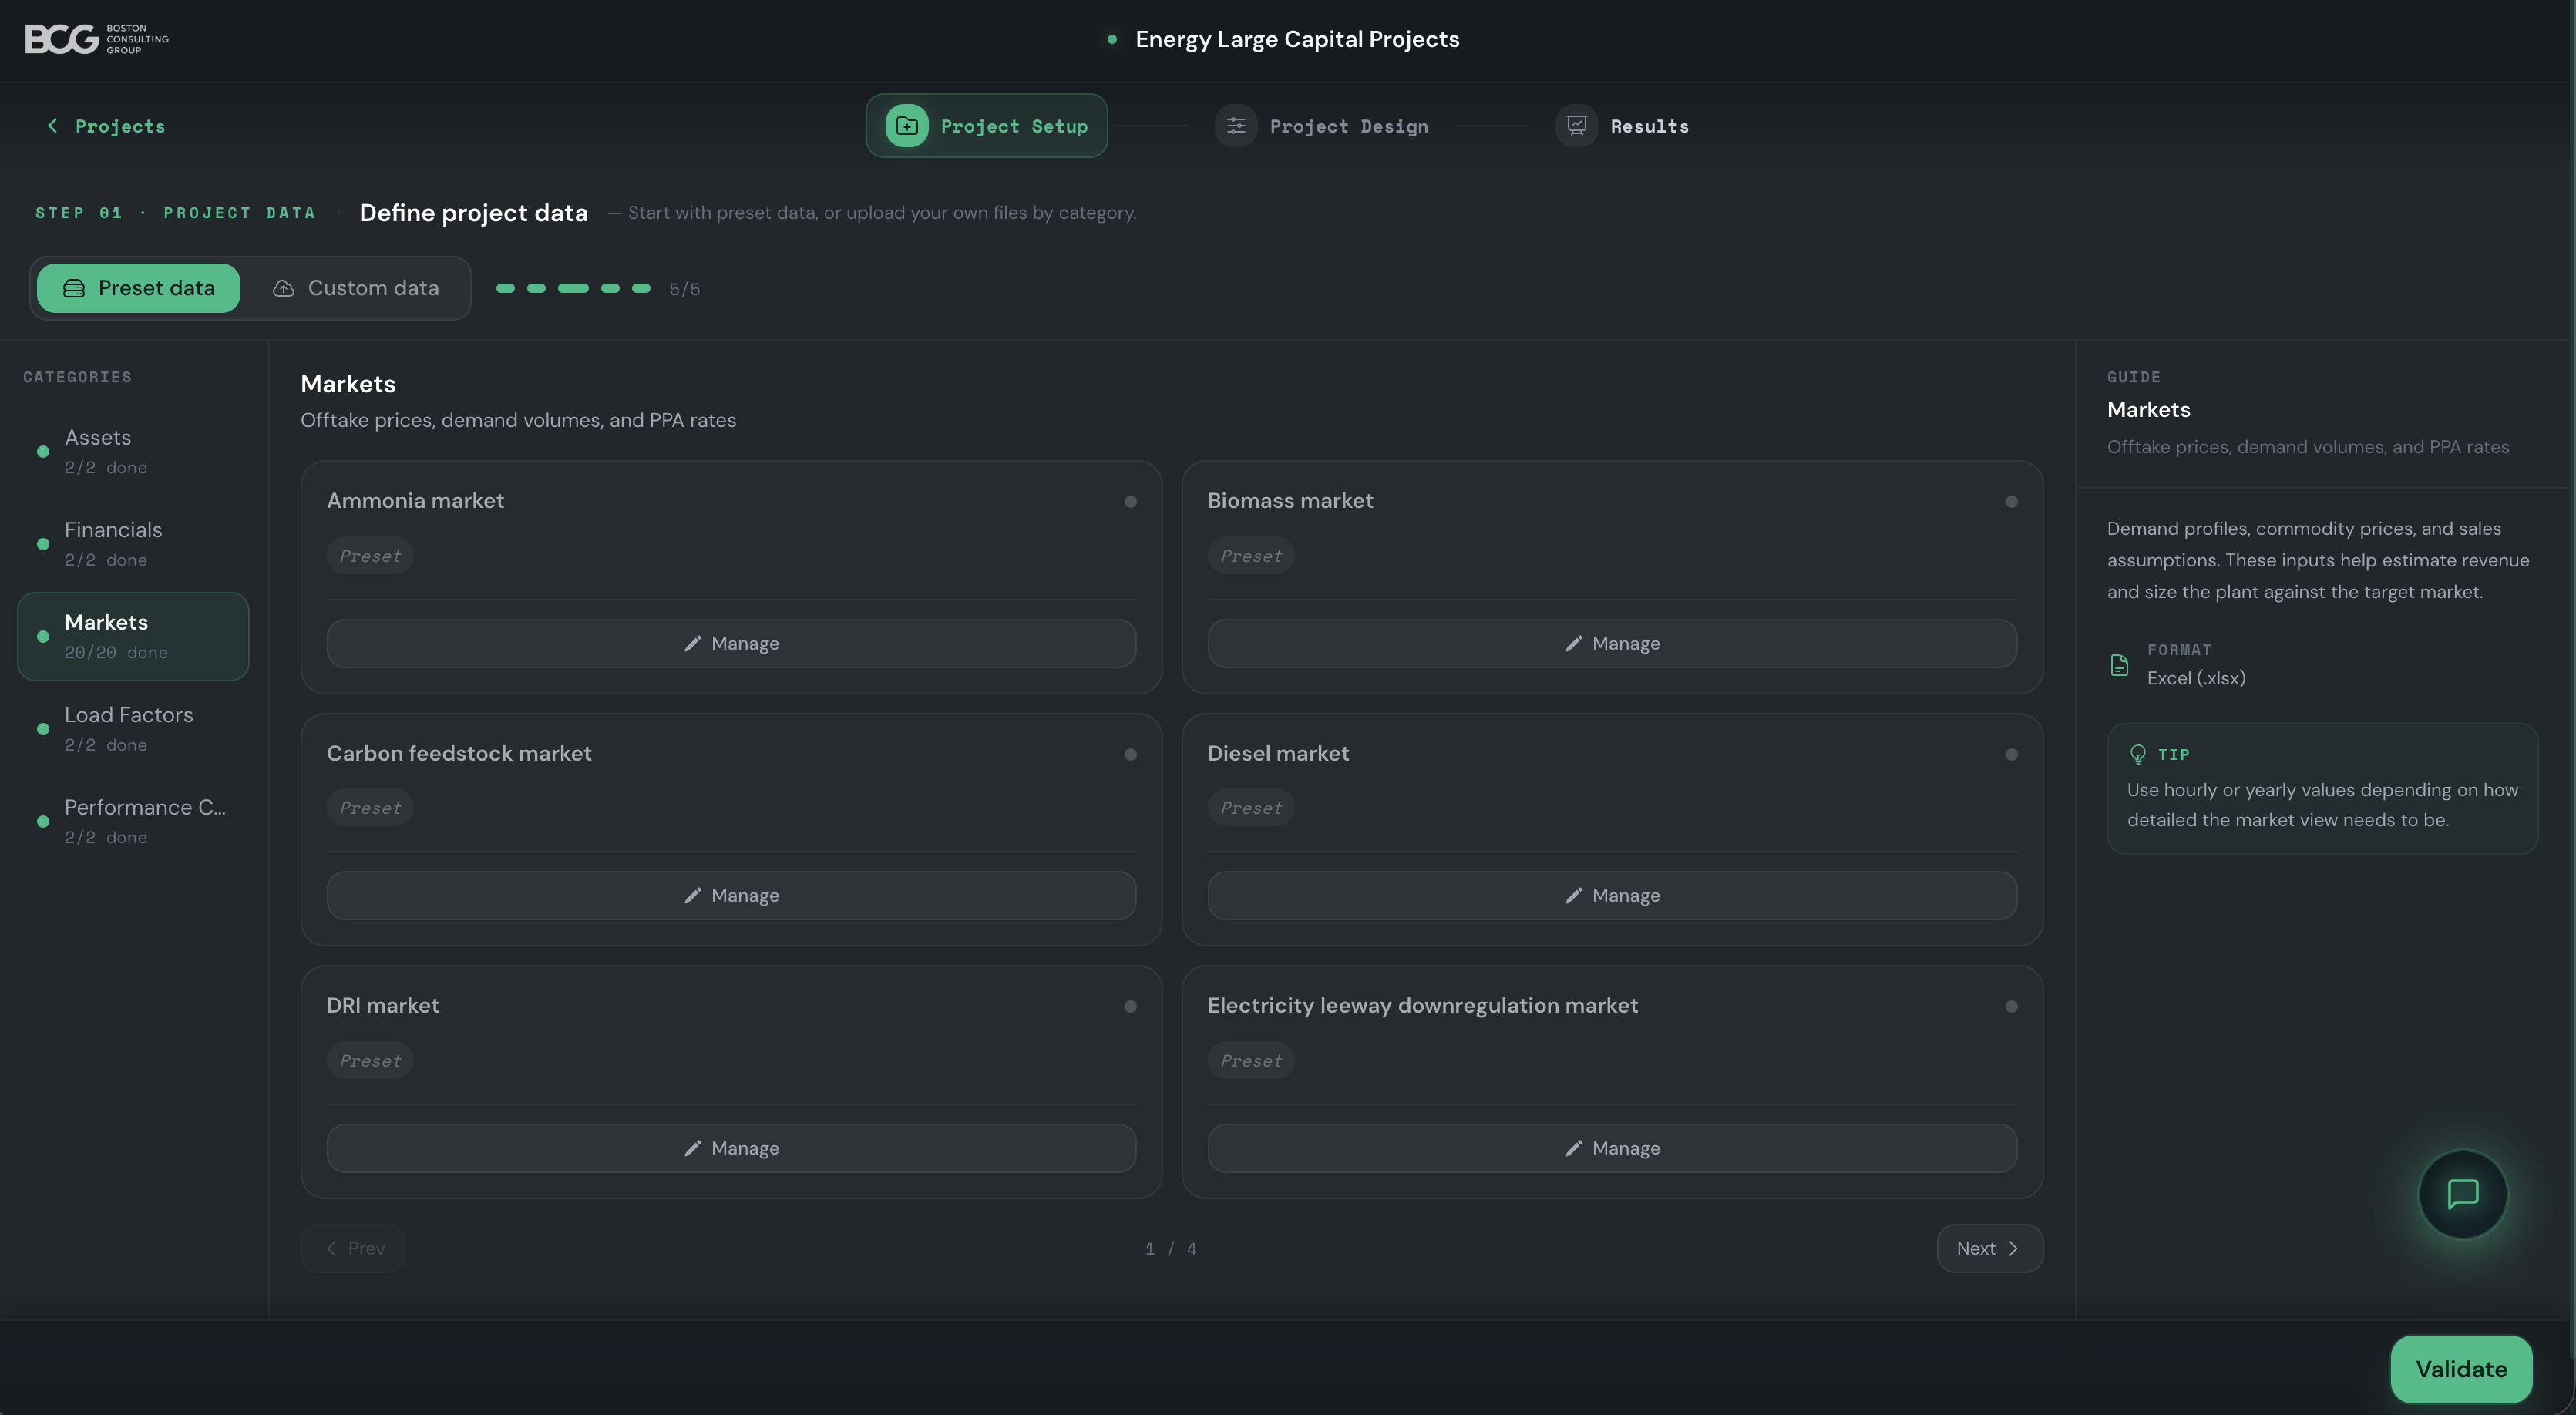
\includegraphics[width=0.95\linewidth]{Figures/chadi_project_data.png}
  \caption{Project data: assets, markets, financing, taxes, and performance inputs.}
  \label{fig:impl-data}
\end{figure}

\begin{figure}[H]
  \centering
  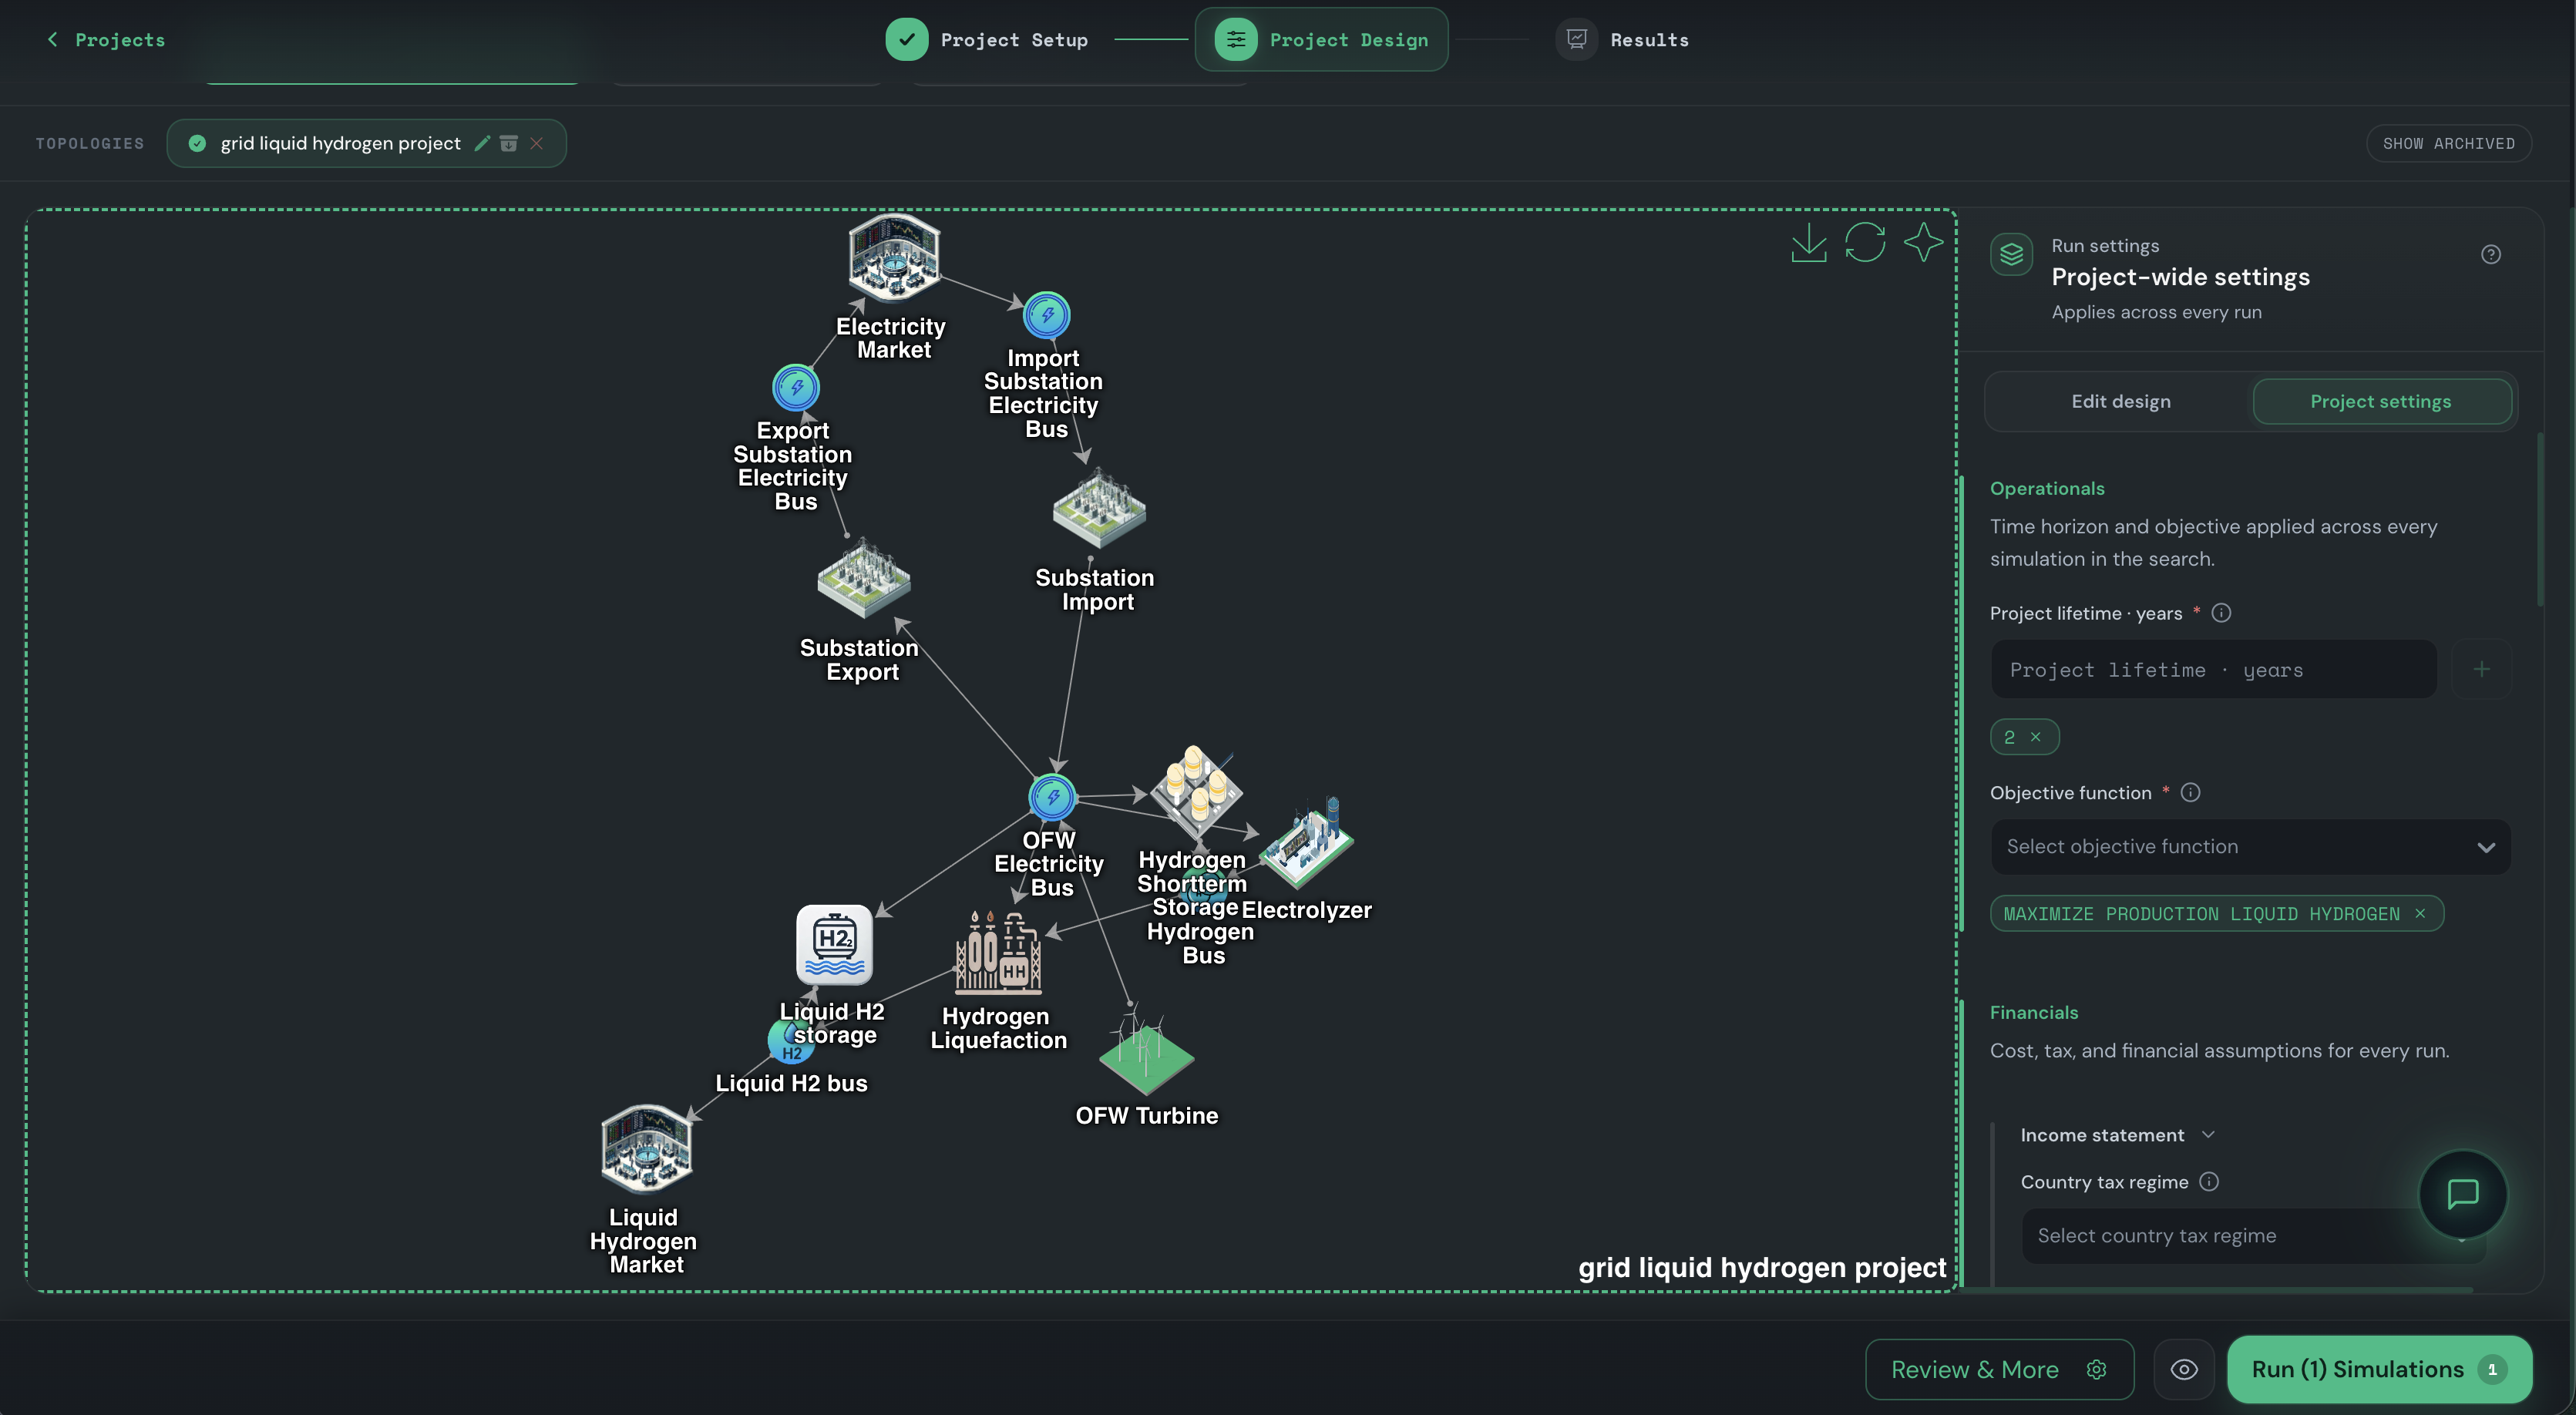
\includegraphics[width=0.95\linewidth]{Figures/chadi_topology_workspace.png}
  \caption{Topology workspace: the project graph, editable and the launch point for simulations.}
  \label{fig:impl-topo}
\end{figure}

\begin{figure}[H]
  \centering
  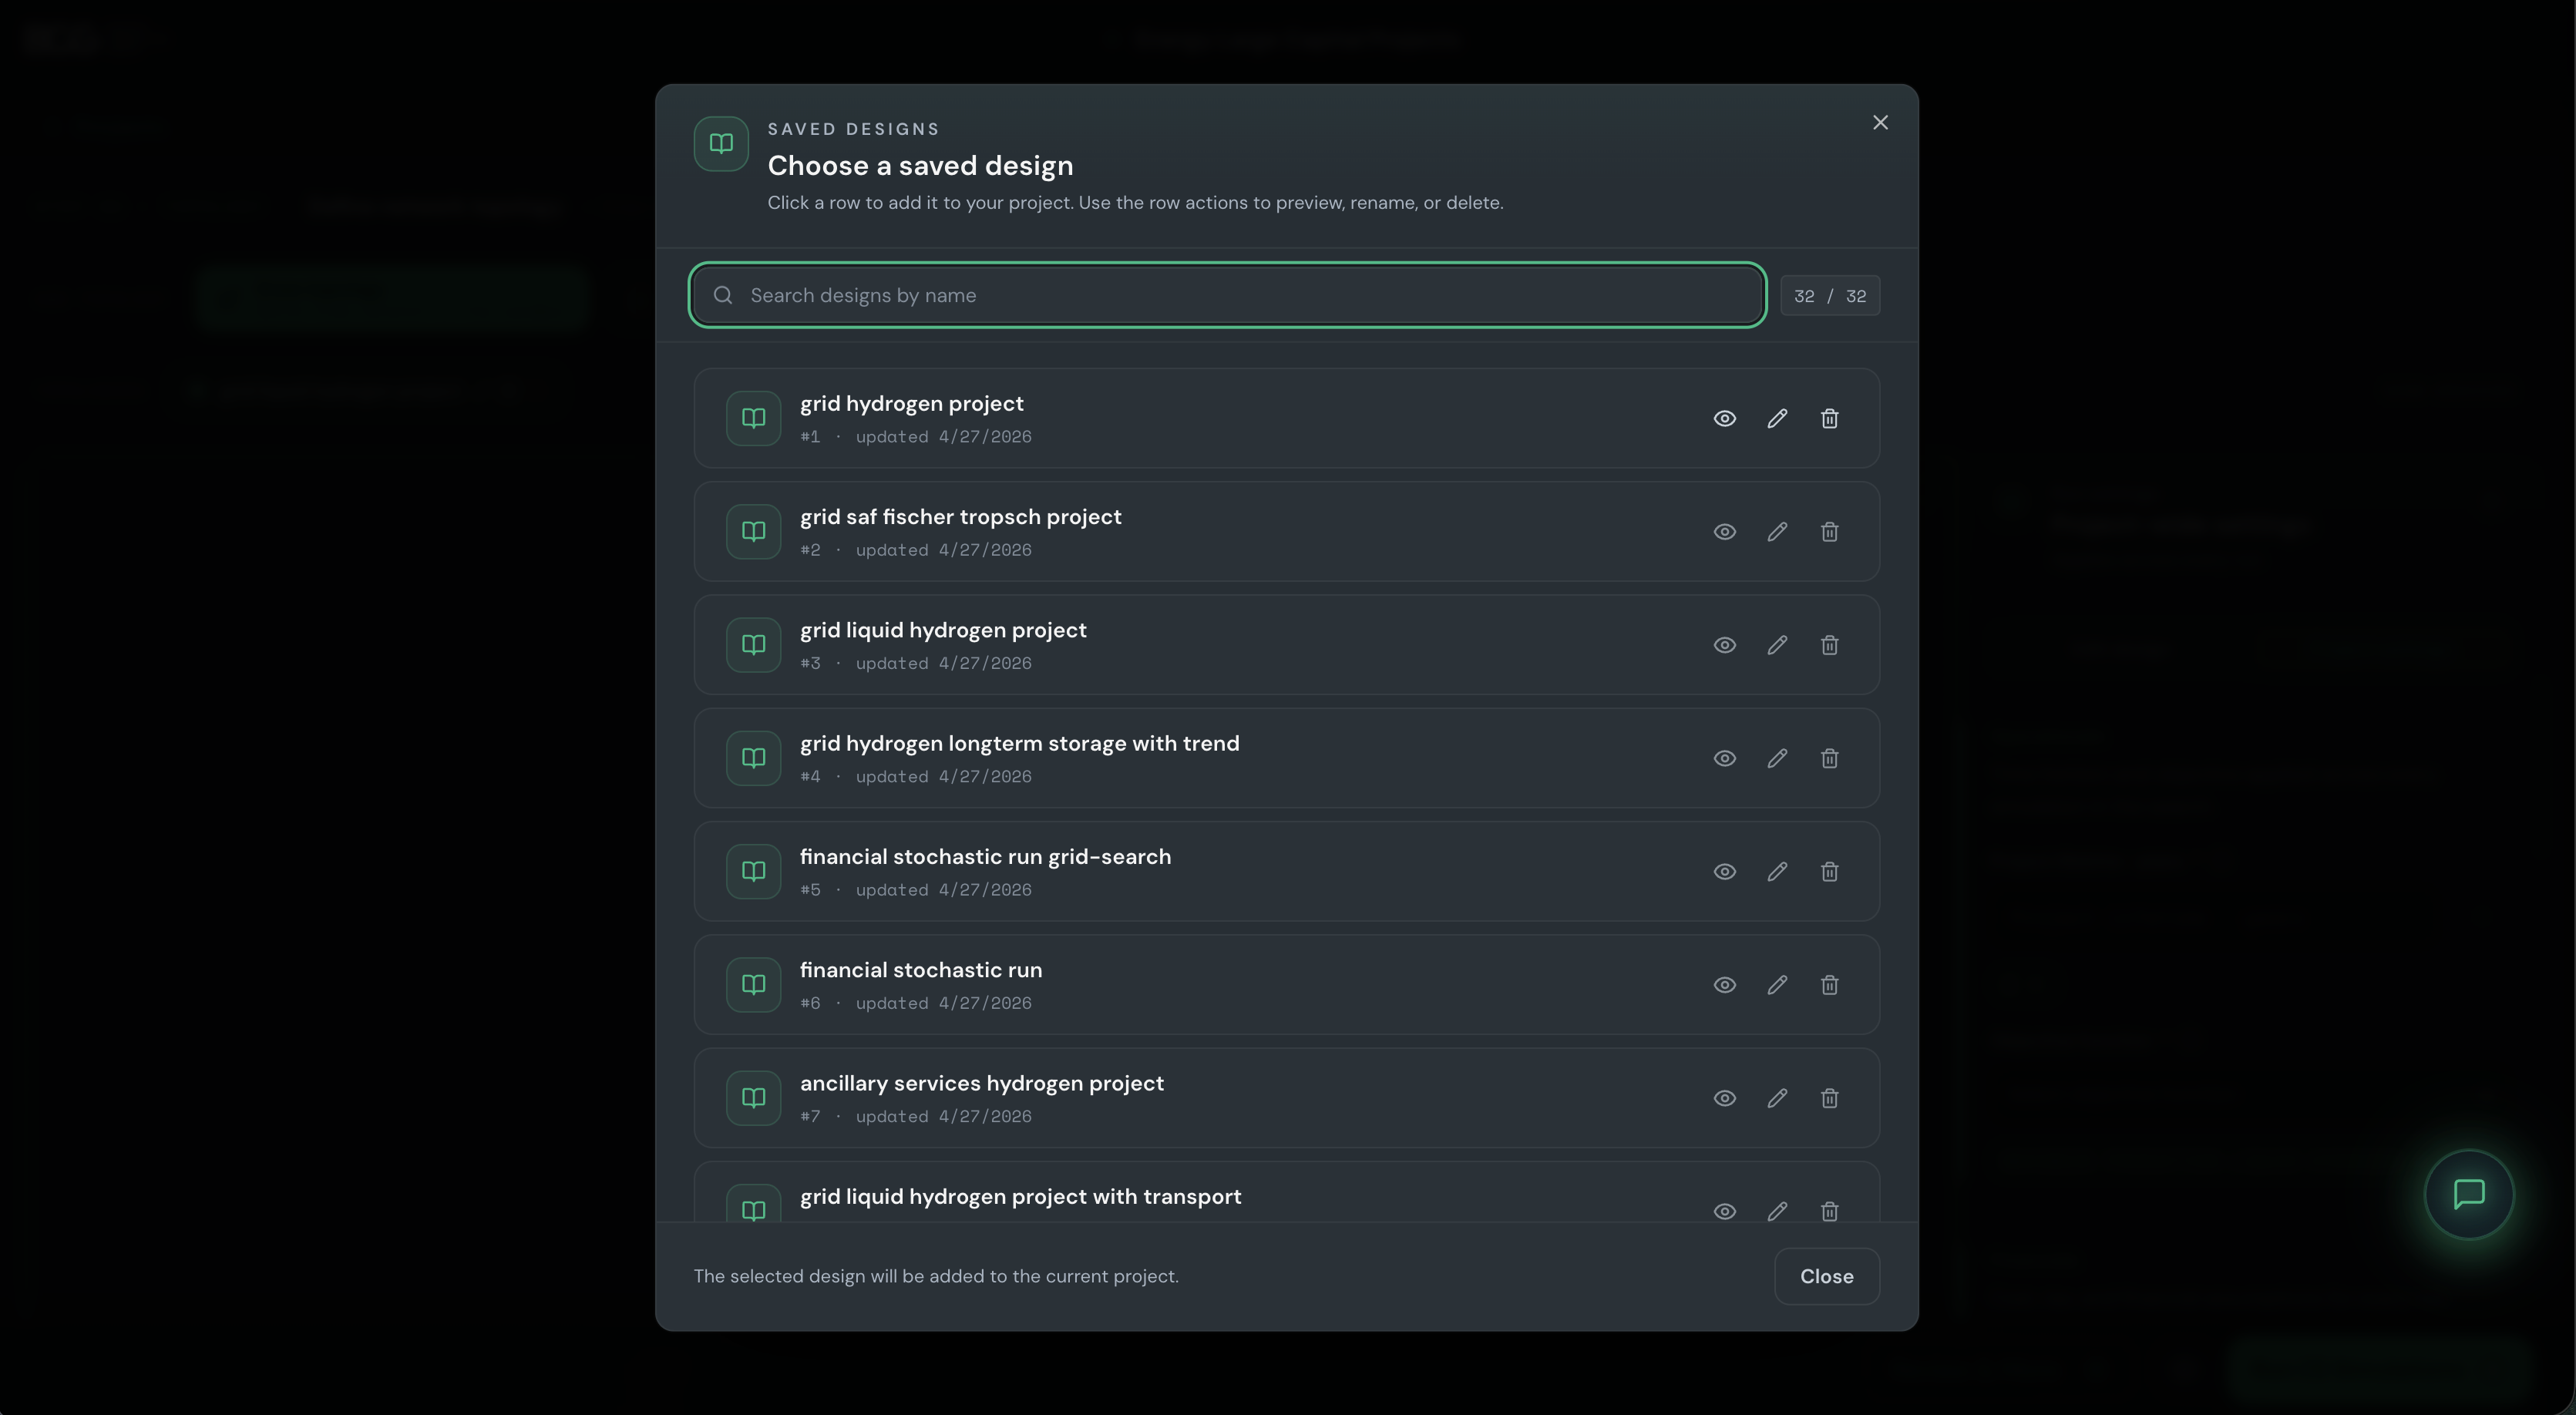
\includegraphics[width=0.95\linewidth]{Figures/chadi_saved_designs.png}
  \caption{Saved designs: reusable topology templates as starting points.}
  \label{fig:impl-saved}
\end{figure}

\begin{figure}[H]
  \centering
  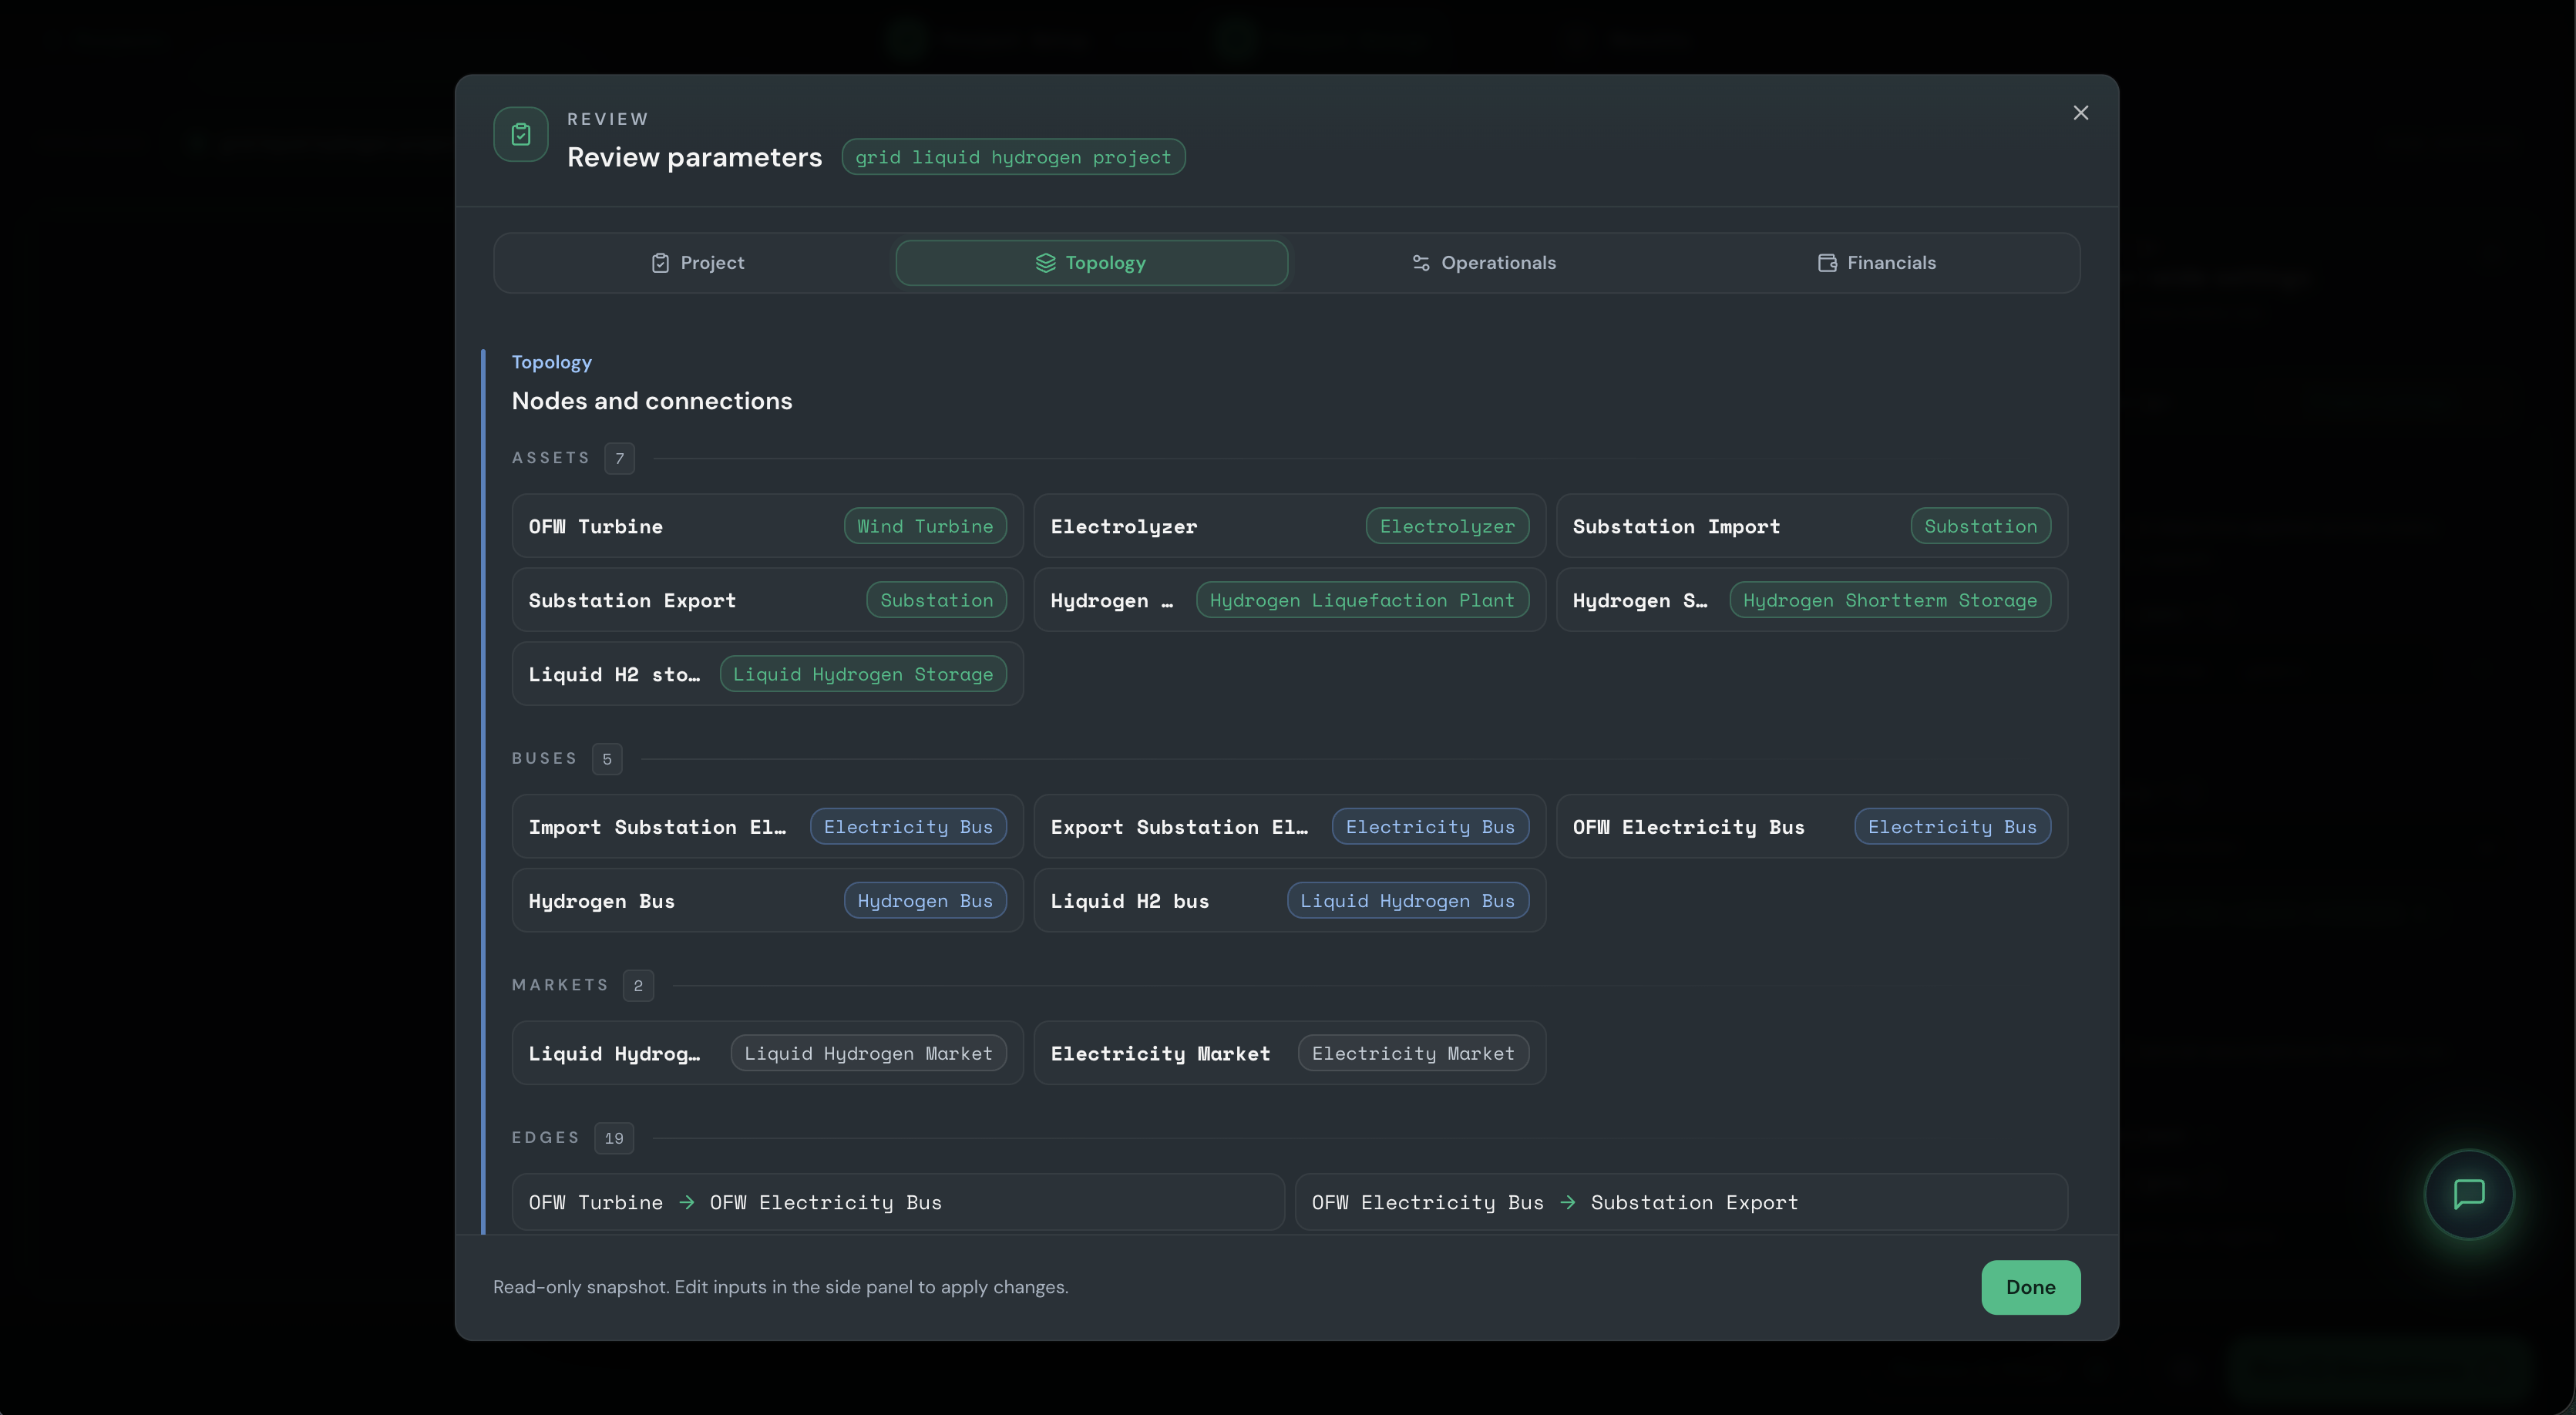
\includegraphics[width=0.95\linewidth]{Figures/chadi_topology_params.png}
  \caption{Topology parameters: component-level assumptions the engine consumes.}
  \label{fig:impl-topoparams}
\end{figure}

\begin{figure}[H]
  \centering
  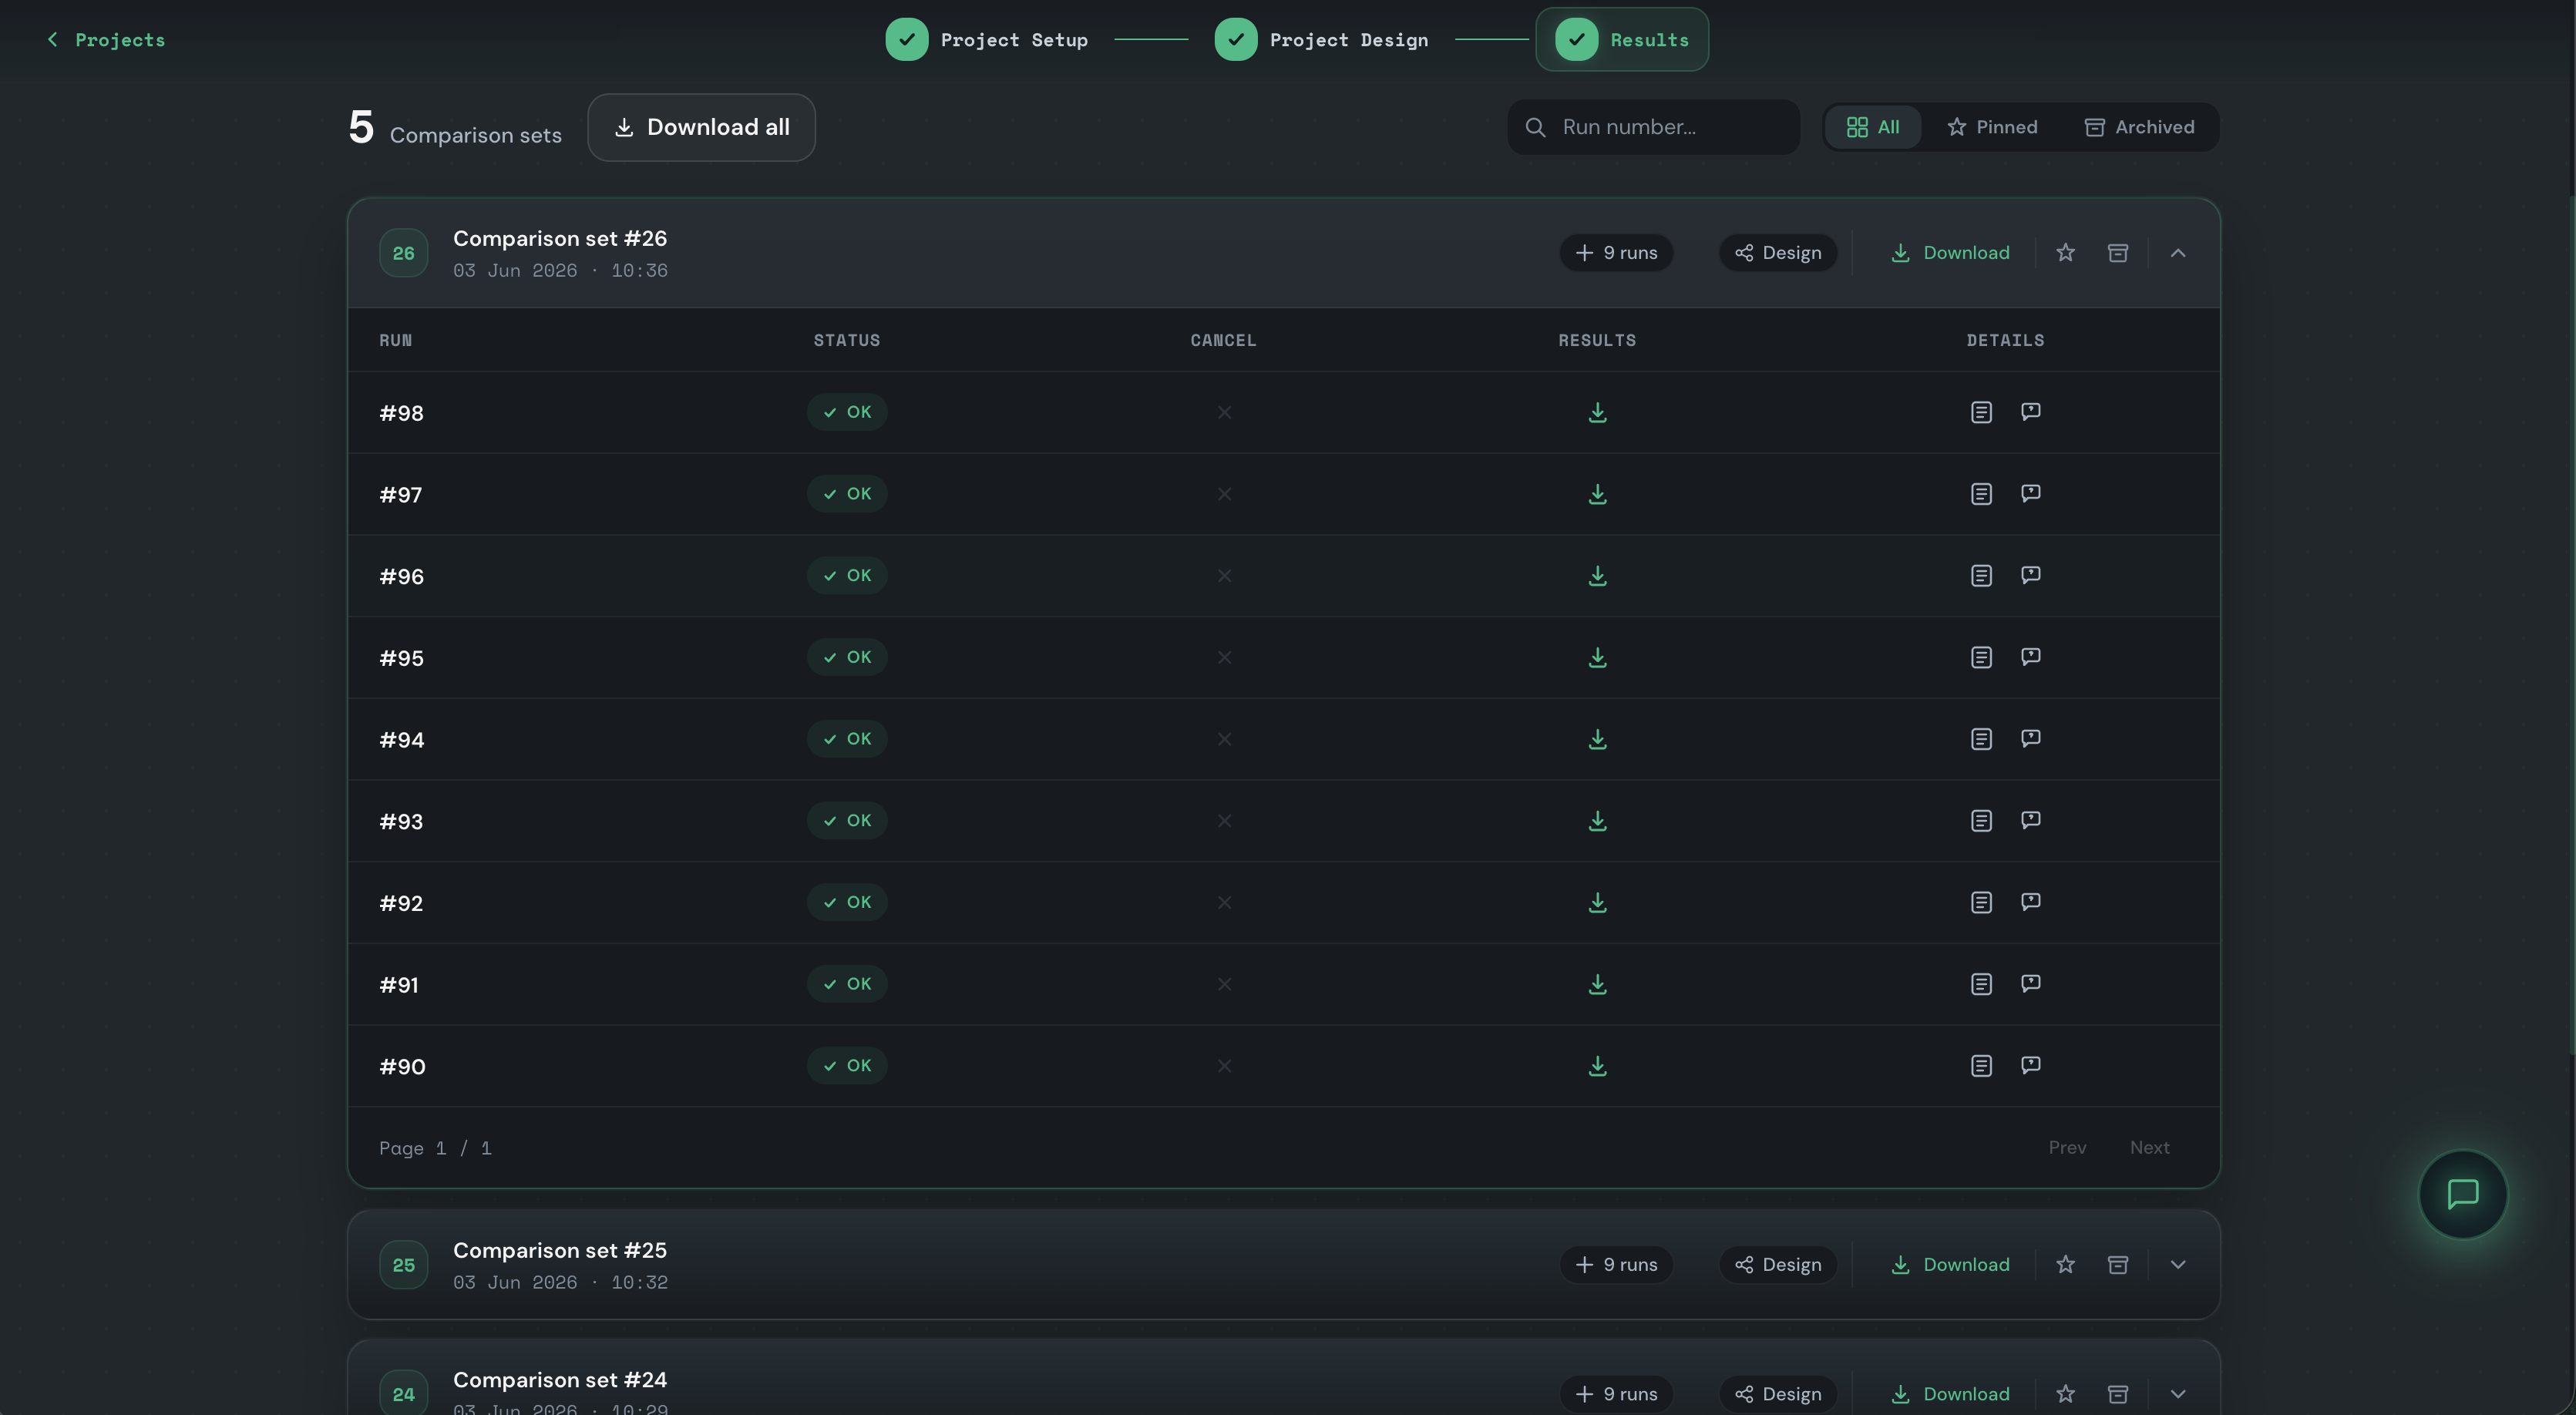
\includegraphics[width=0.95\linewidth]{Figures/chadi_comparison_table.png}
  \caption{Comparison table: deterministic outputs across runs in a dense review format.}
  \label{fig:impl-comptable}
\end{figure}

\begin{figure}[H]
  \centering
  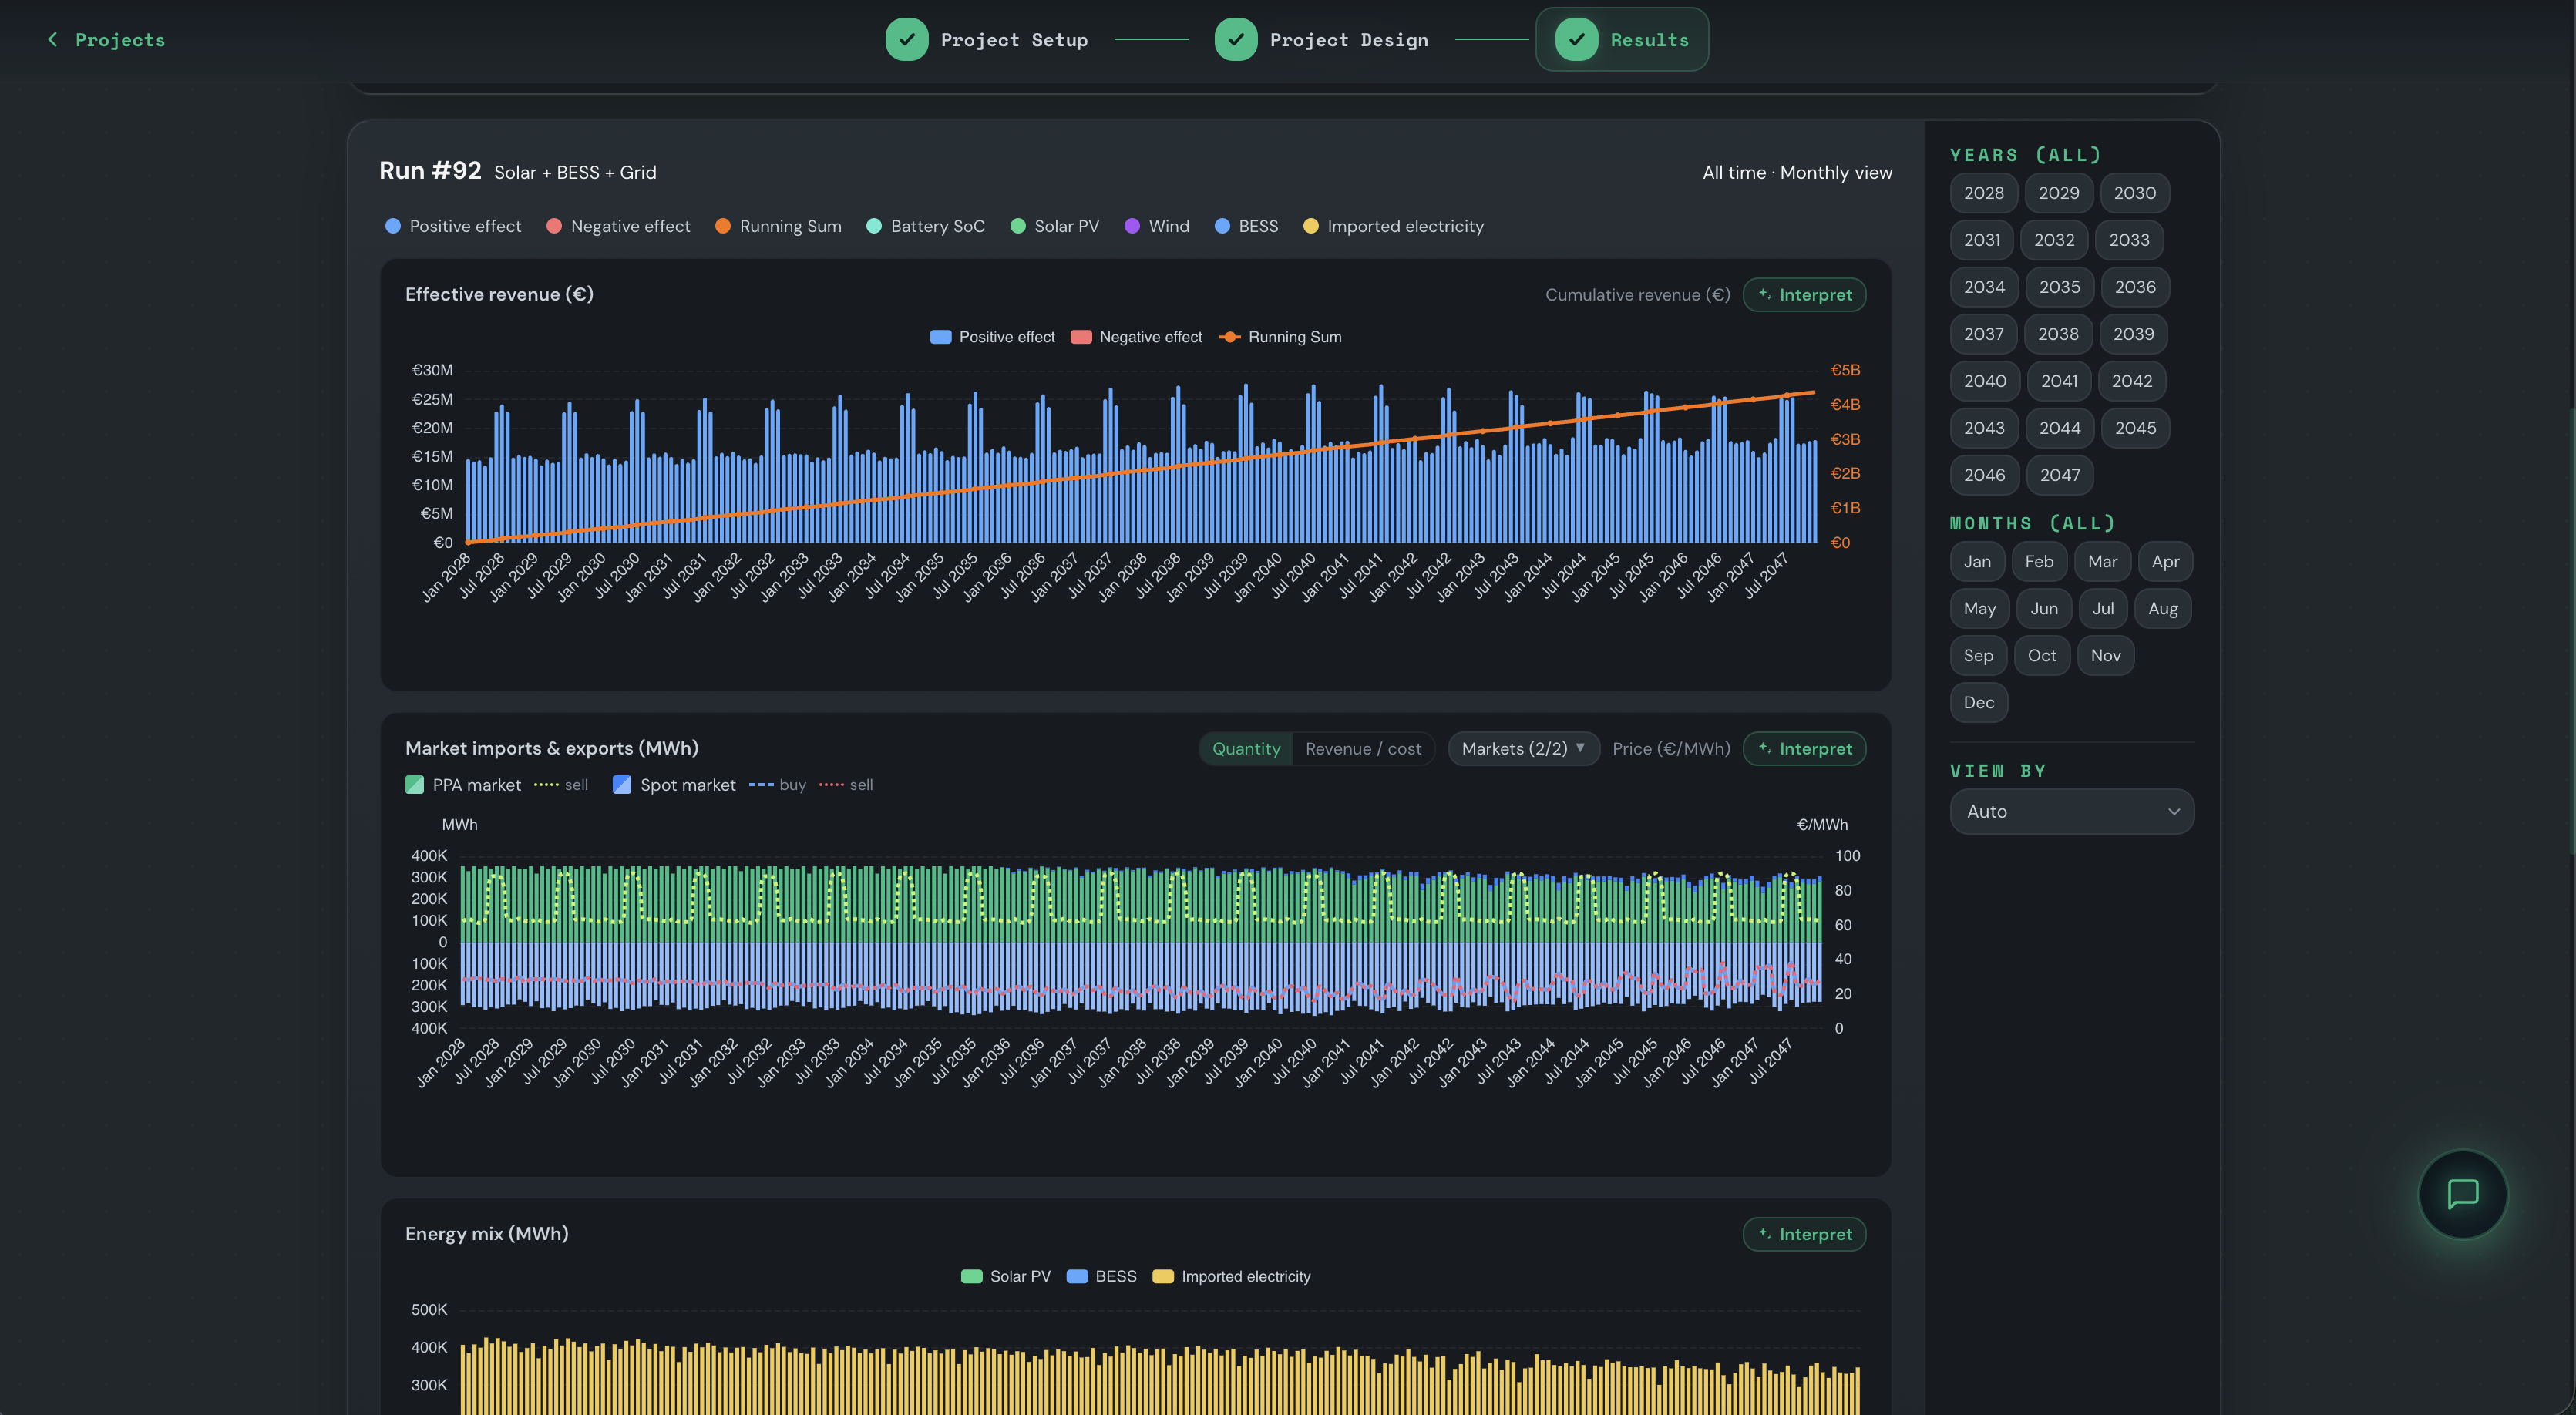
\includegraphics[width=0.95\linewidth]{Figures/chadi_run_charts.png}
  \caption{Run charts: effective revenue and market imports and exports with time filters.}
  \label{fig:impl-runcharts}
\end{figure}

\subsection{Agentic project creation}

Once the restored application path is visible, the sequence shifts to the agentic
layer. The first conversation demonstrates discovery, intent capture, and
approval-gated creation
(Figures~\ref{fig:impl-agentpanel}--\ref{fig:impl-postapproval}). The
implementation point is control: the agent helps the user move faster, but
important state changes still pass through explicit proposal and approval steps.

\begin{figure}[H]
  \centering
  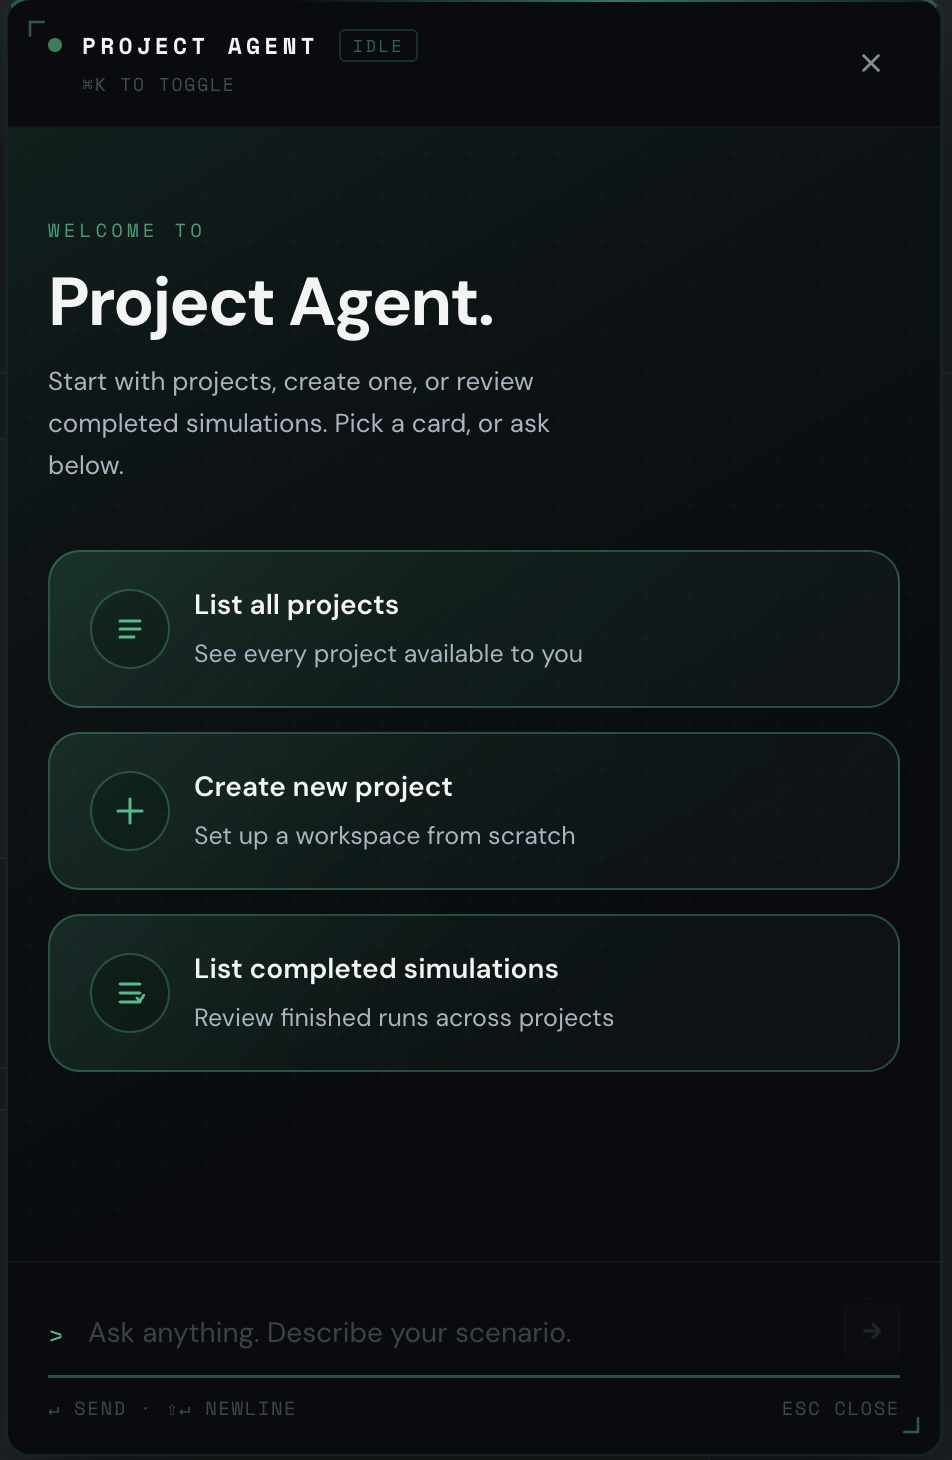
\includegraphics[width=0.48\linewidth]{Figures/chadi_agent_panel.png}
  \caption{Agent command panel: guided entry points and a free-form prompt.}
  \label{fig:impl-agentpanel}
\end{figure}

\begin{figure}[H]
  \centering
  
\includegraphics[width=0.62\linewidth]{Figures/chadi_intent_capture.png}
  \caption{Intent capture: the agent asks for a topic, geography, year, or technology cue.}
  \label{fig:impl-intent}
\end{figure}

\begin{figure}[H]
  \centering
  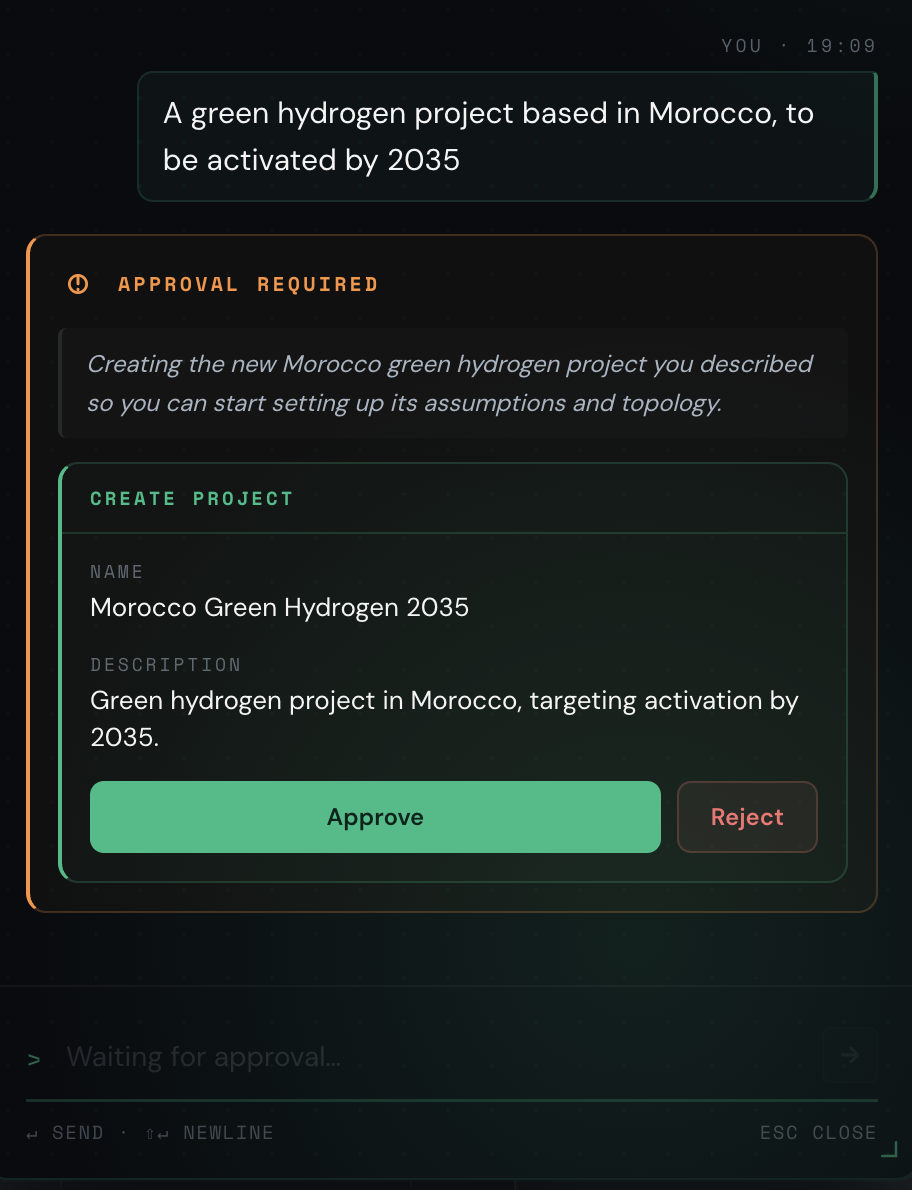
\includegraphics[width=0.5\linewidth]{Figures/chadi_approval_card.png}
  \caption{Approval card: a proposed project awaits approval, the first governed write.}
  \label{fig:impl-approval}
\end{figure}

\begin{figure}[H]
  \centering
  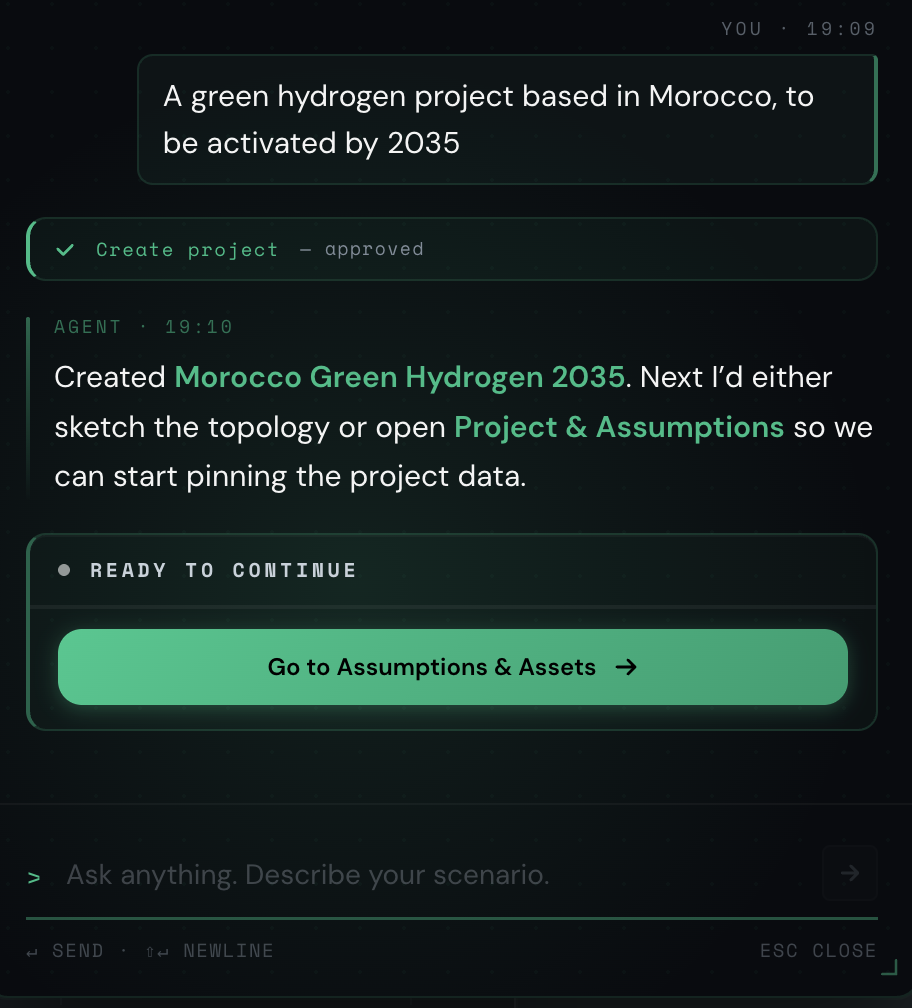
\includegraphics[width=0.55\linewidth]{Figures/chadi_post_approval.png}
  \caption{Post-approval: an approved proposal becomes a concrete product transition.}
  \label{fig:impl-postapproval}
\end{figure}

\subsection{File and assumption ingestion}

Uploaded assumptions can change simulation results directly, so ingestion is a
governed workflow that combines conversational guidance with explicit file review:
the assistant reads project state and reasons about differences, while the
application surfaces previews, matches, conflicts, and review gates before any data
is accepted (Figures~\ref{fig:impl-context}--\ref{fig:impl-review}).

\begin{figure}[H]
  \centering
  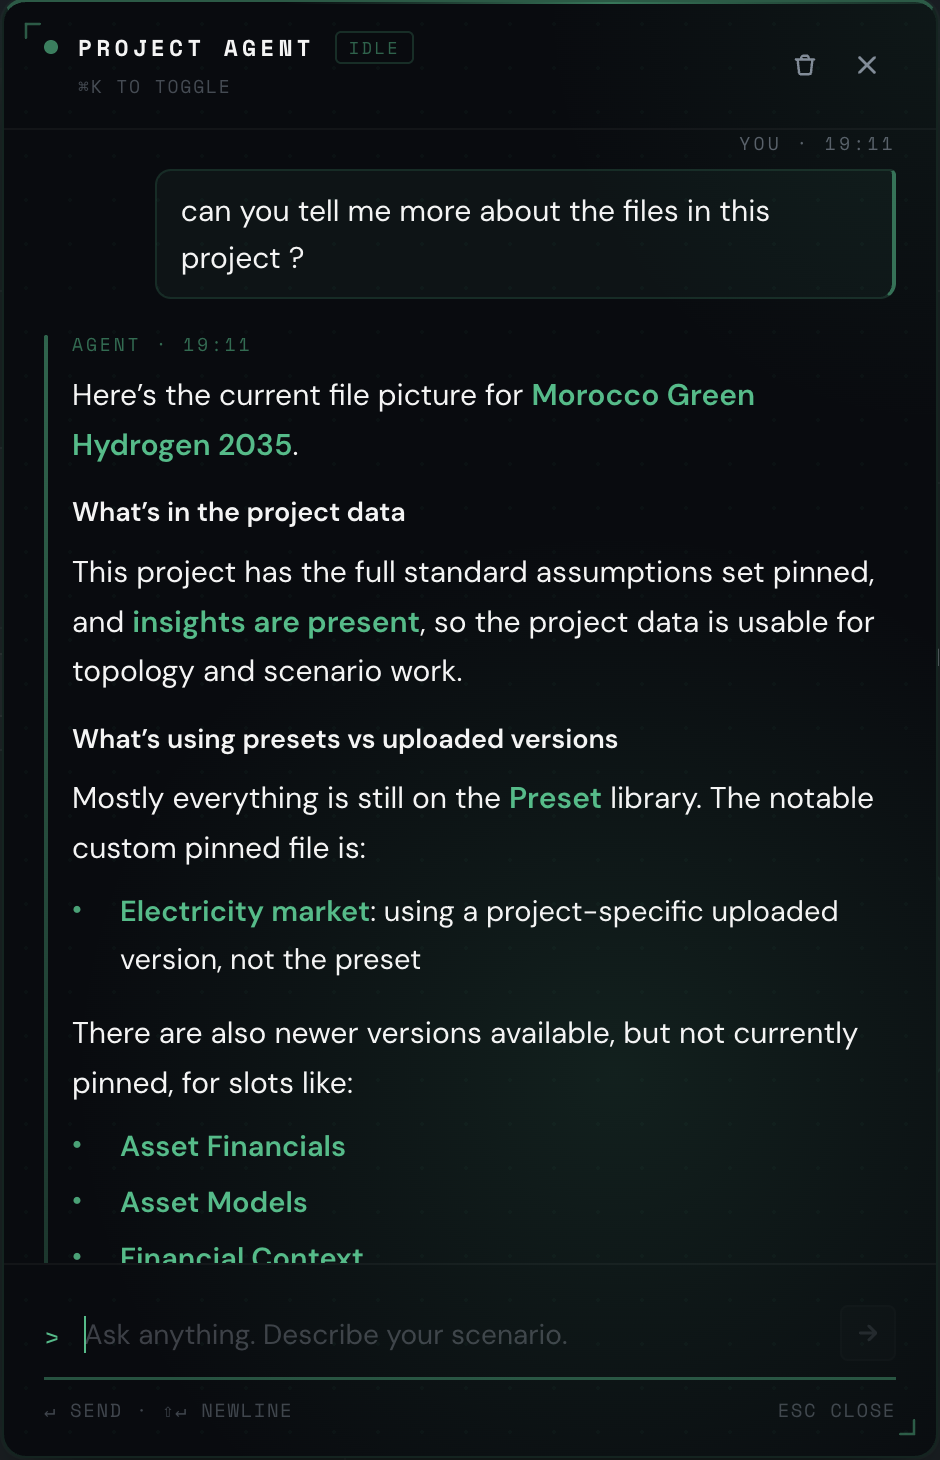
\includegraphics[width=0.48\linewidth]{Figures/chadi_context_retrieval.png}
  \caption{Context retrieval: which assumption files and versions are attached.}
  \label{fig:impl-context}
\end{figure}

\begin{figure}[H]
  \centering
  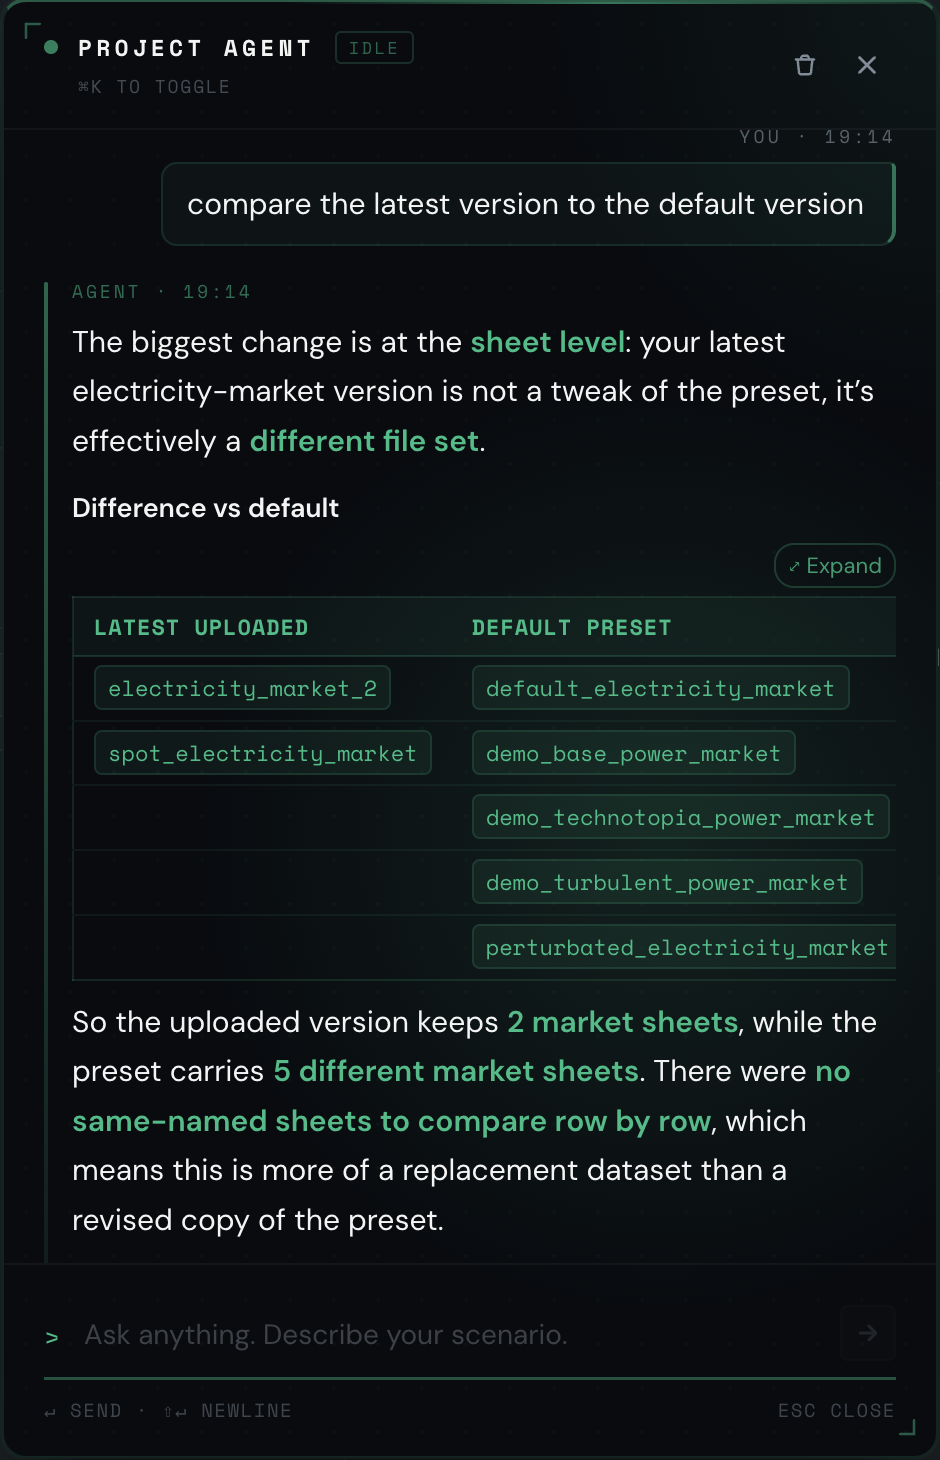
\includegraphics[width=0.48\linewidth]{Figures/chadi_file_comparison.png}
  \caption{File comparison: an uploaded sheet compared with the preset, sheet by sheet.}
  \label{fig:impl-filecomparison}
\end{figure}

\begin{figure}[H]
  \centering
  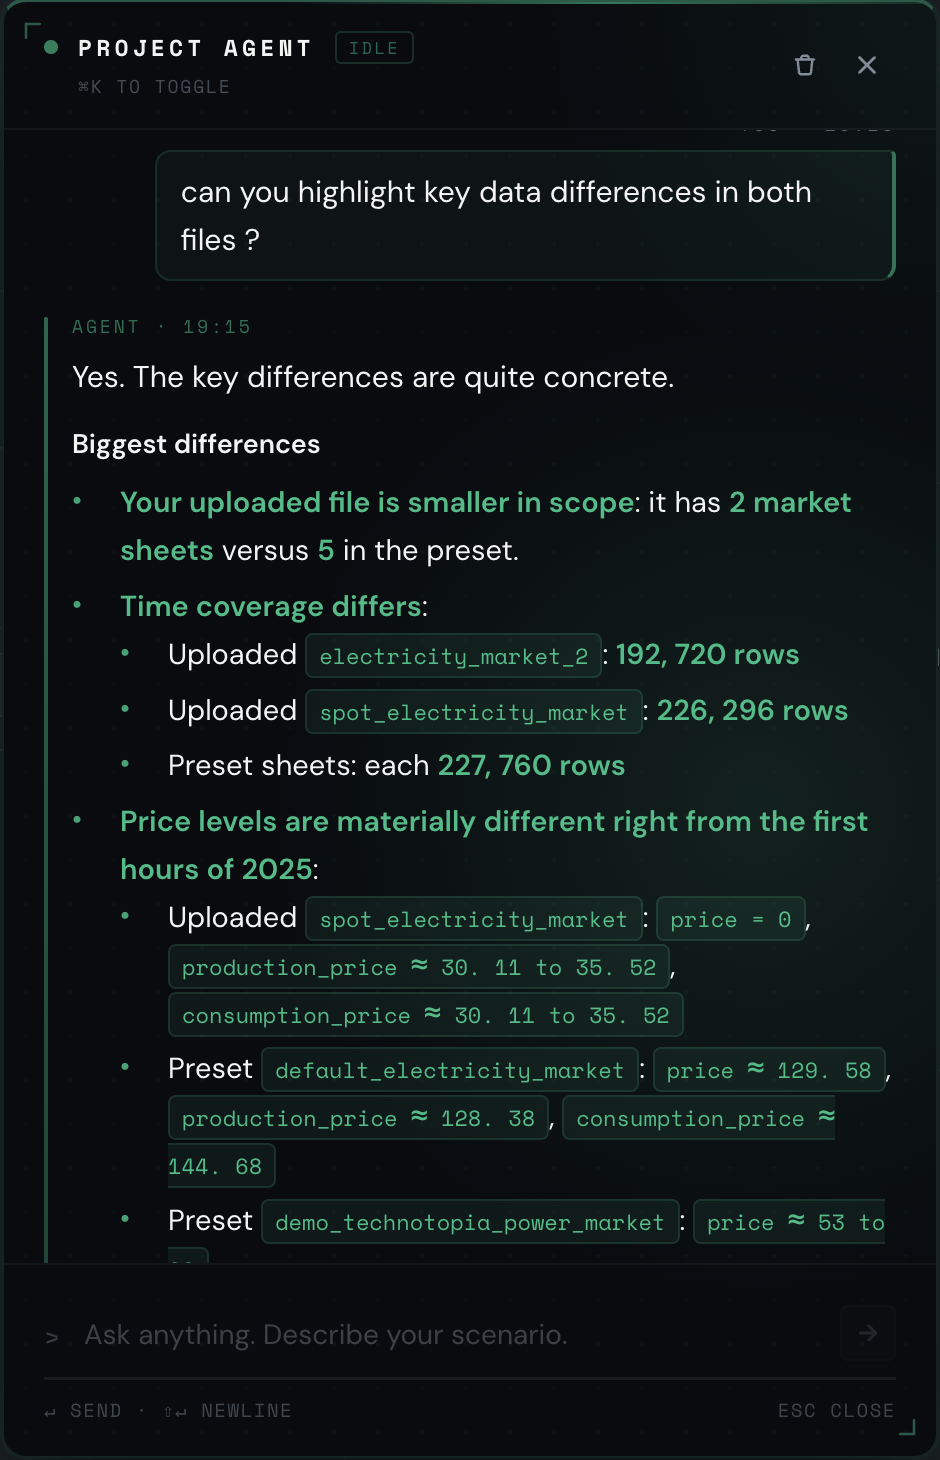
\includegraphics[width=0.48\linewidth]{Figures/chadi_data_differences.png}
  \caption{Data differences: scope, time coverage, and price-level differences made explicit.}
  \label{fig:impl-datadiff}
\end{figure}

\begin{figure}[H]
  \centering
  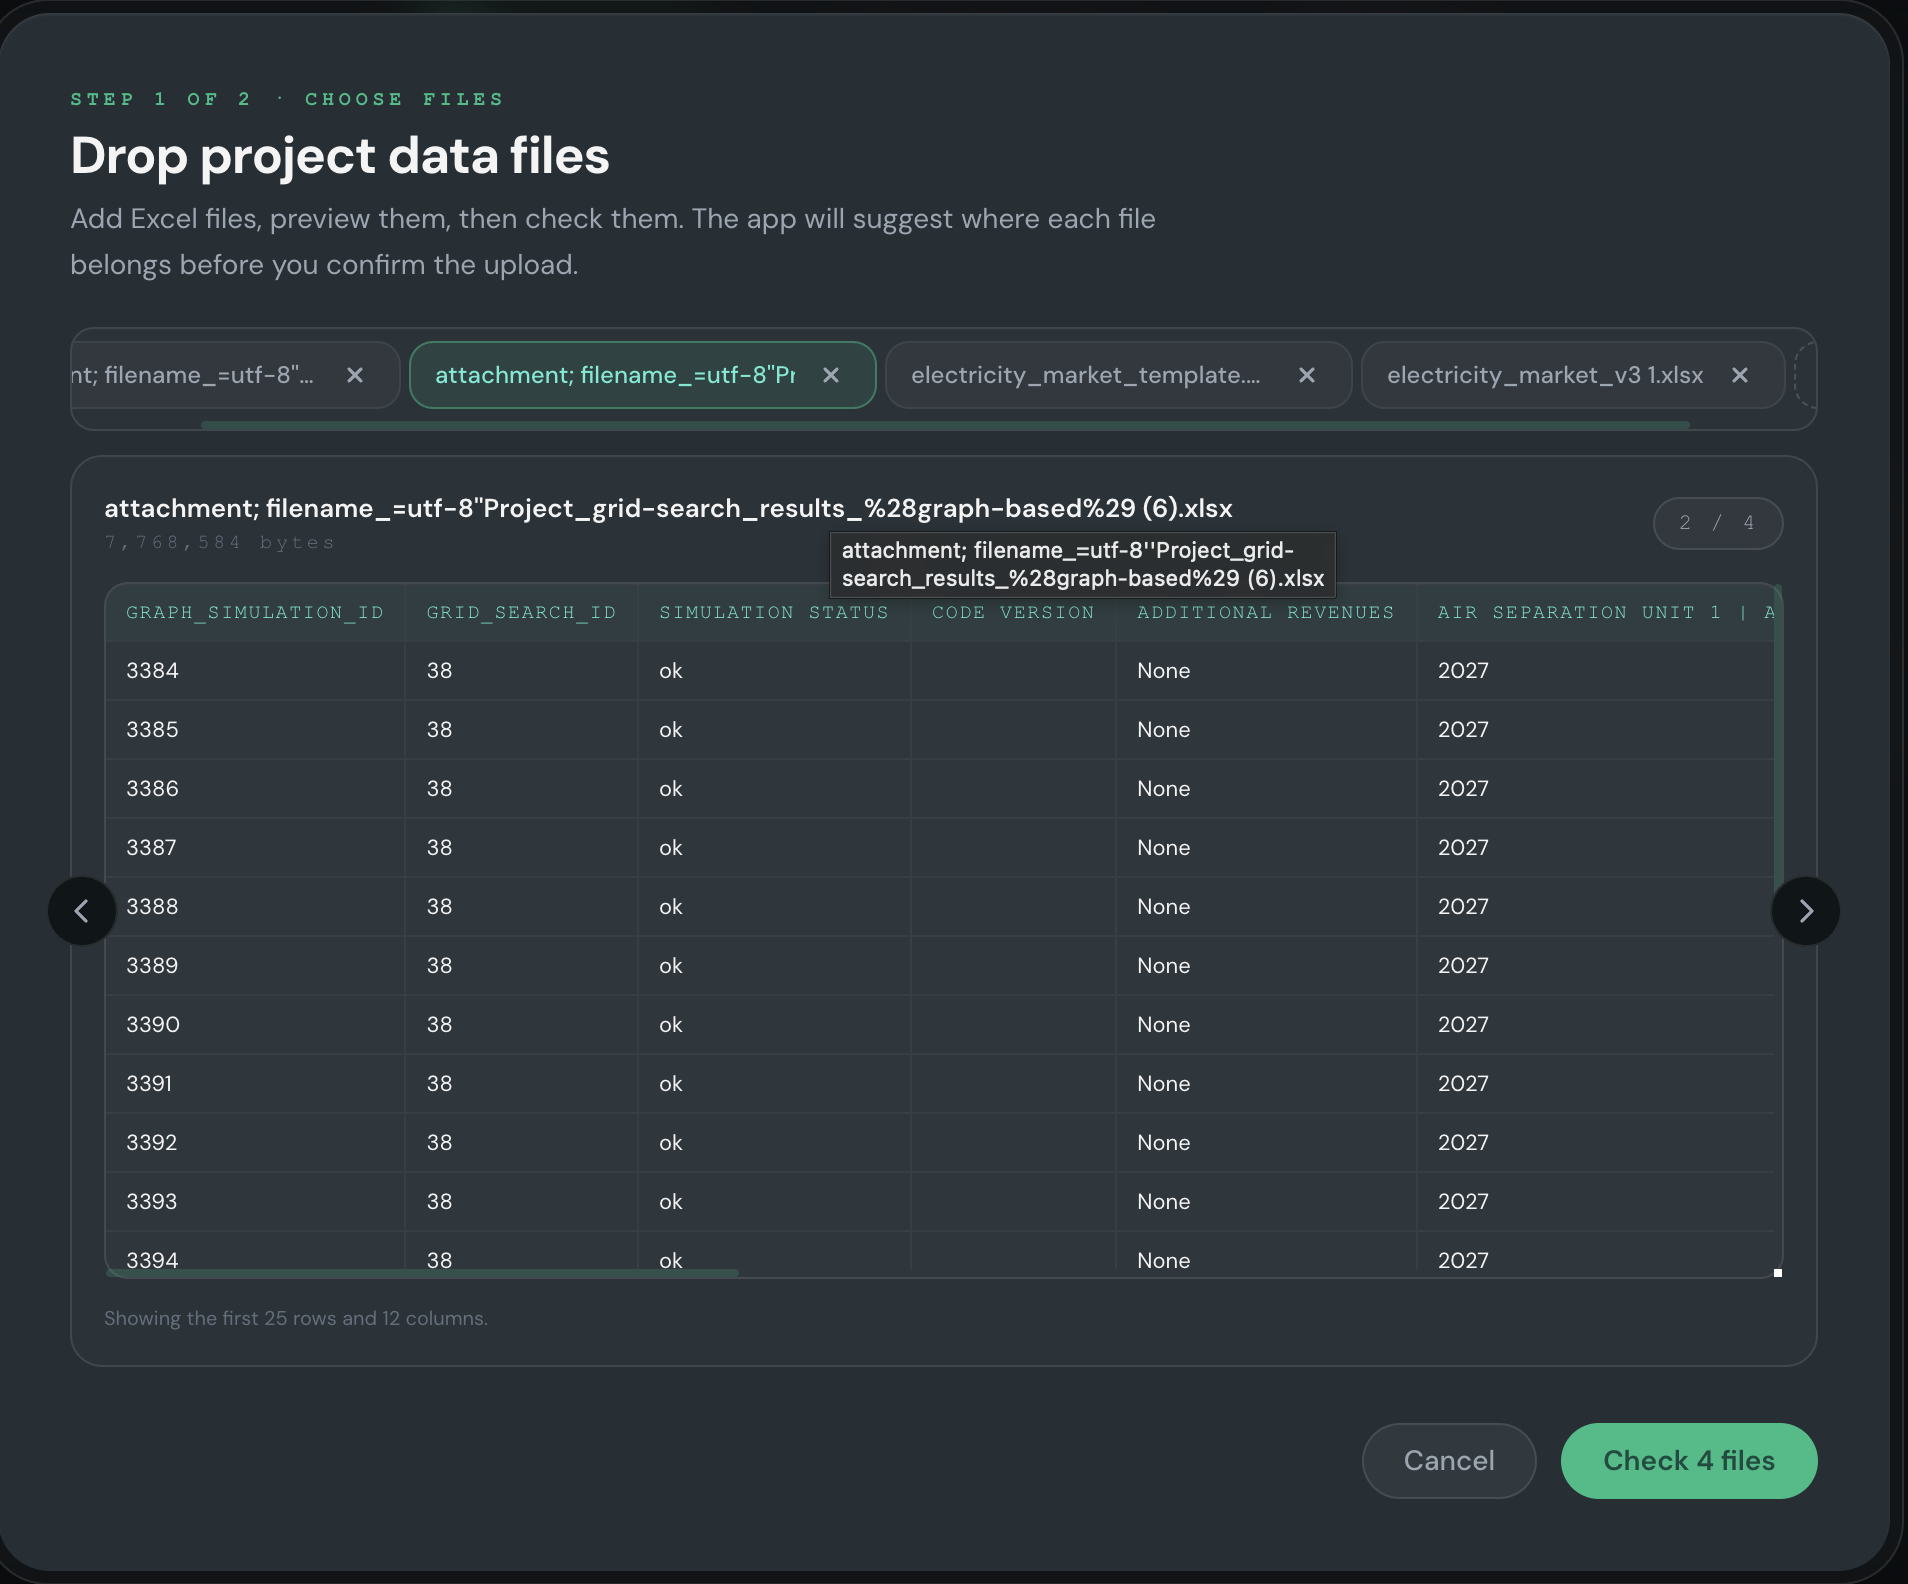
\includegraphics[width=0.72\linewidth]{Figures/chadi_file_preview.png}
  \caption{File preview: workbook and sheet selection with a parsed-row preview.}
  \label{fig:impl-filepreview}
\end{figure}

\begin{figure}[H]
  \centering
  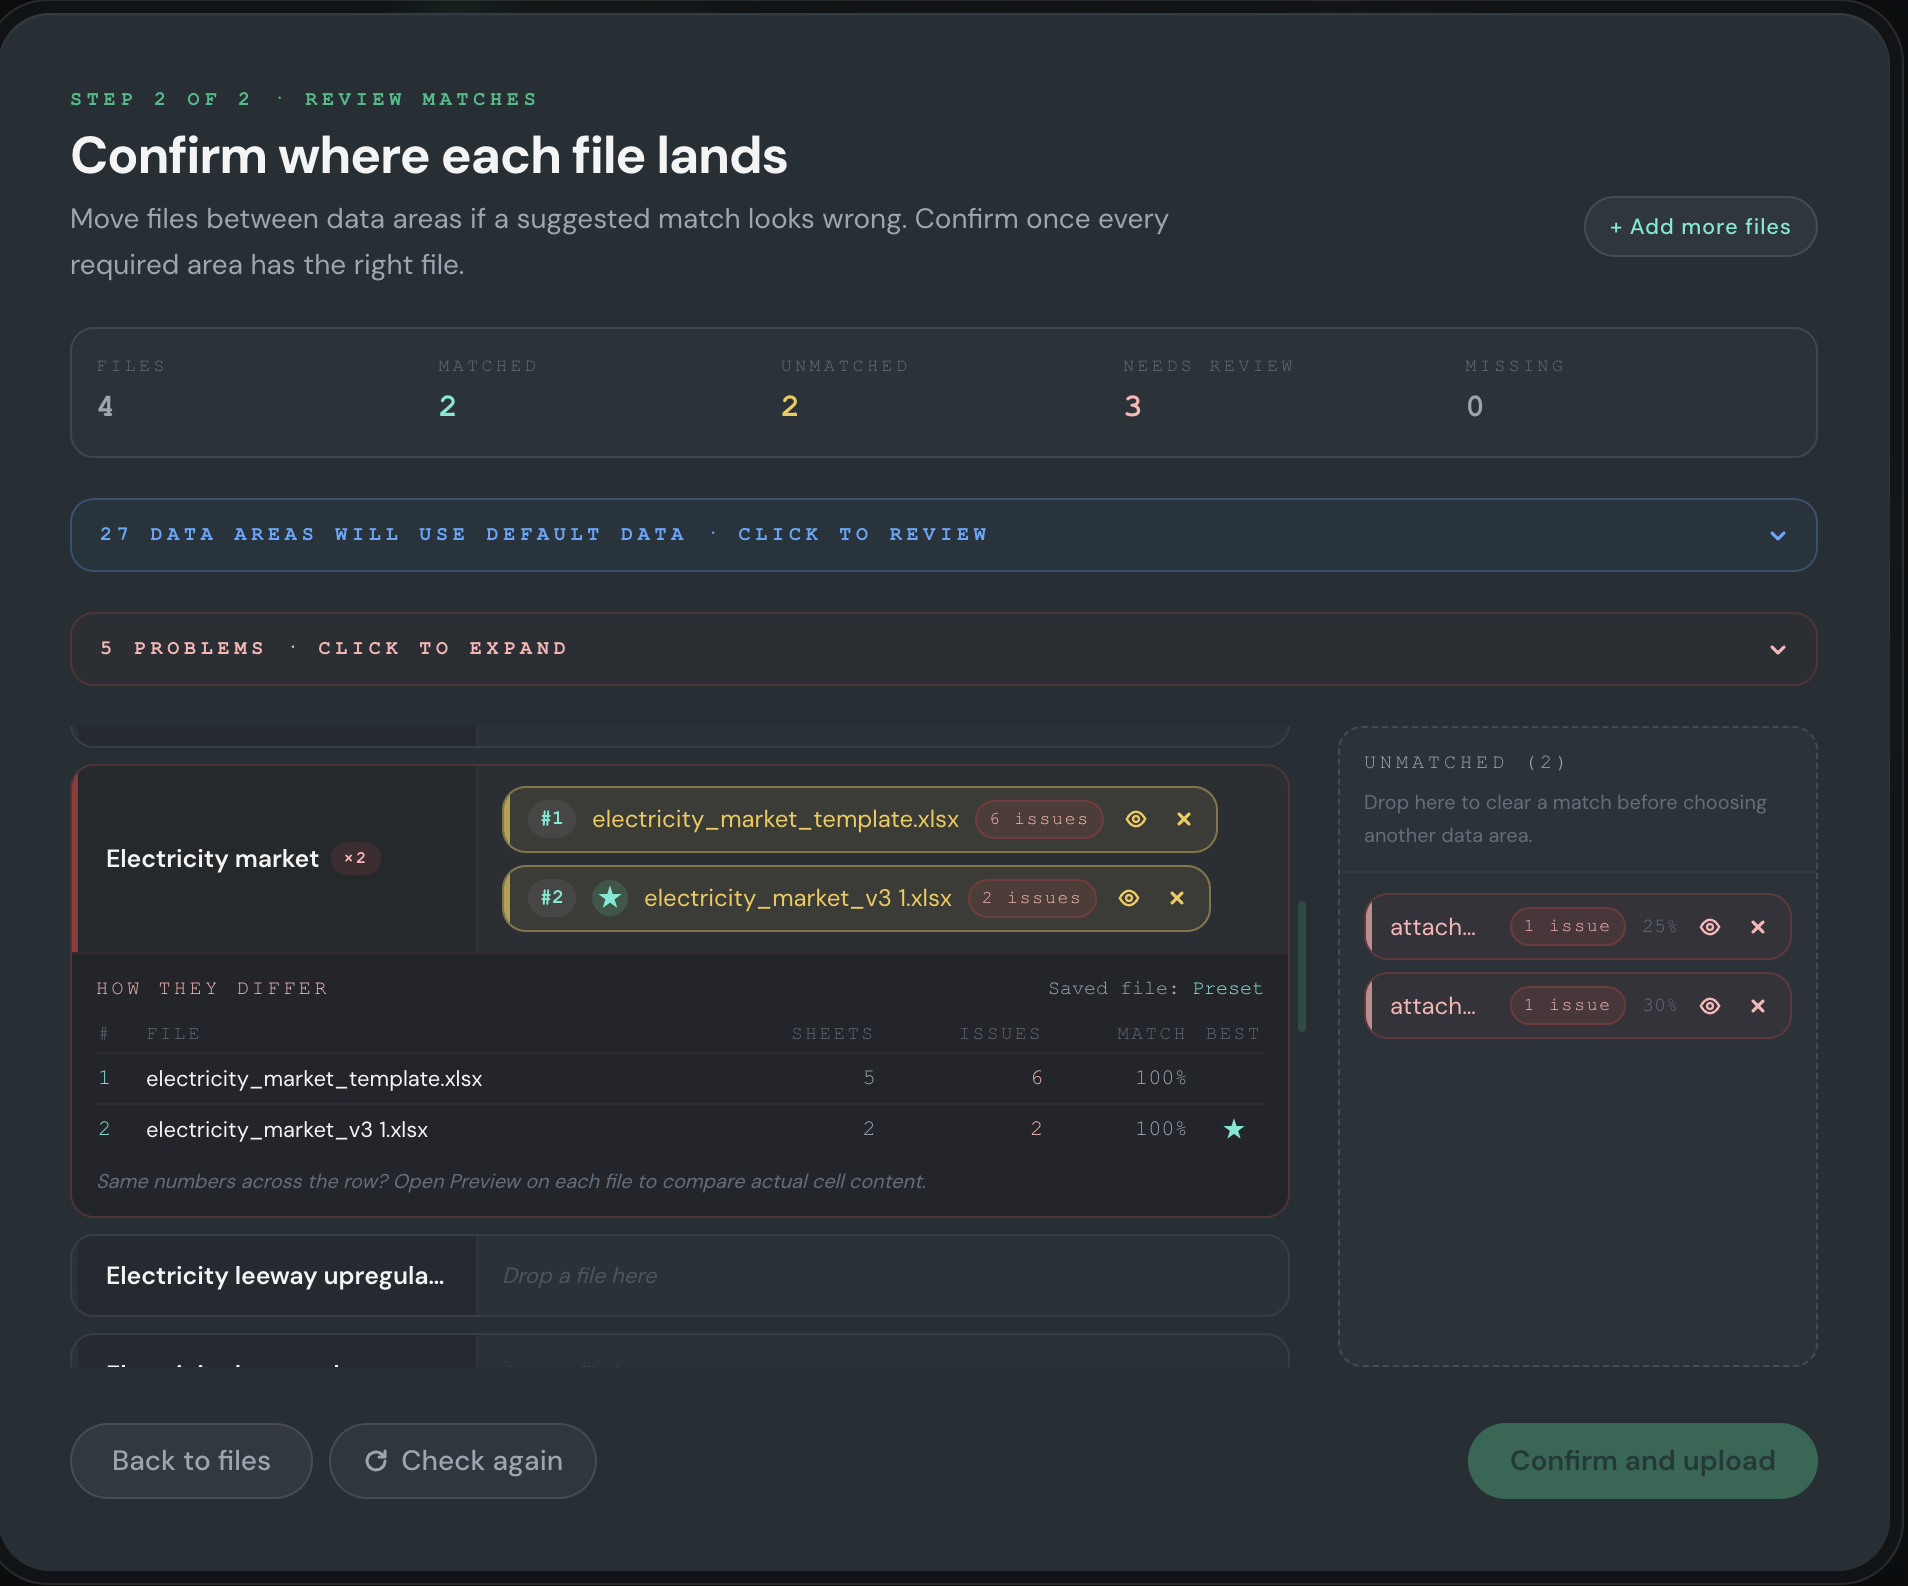
\includegraphics[width=0.72\linewidth]{Figures/chadi_match_confirmation.png}
  \caption{Match confirmation: matched, unmatched, review-needed, and missing areas, gated.}
  \label{fig:impl-match}
\end{figure}

\begin{figure}[H]
  \centering
  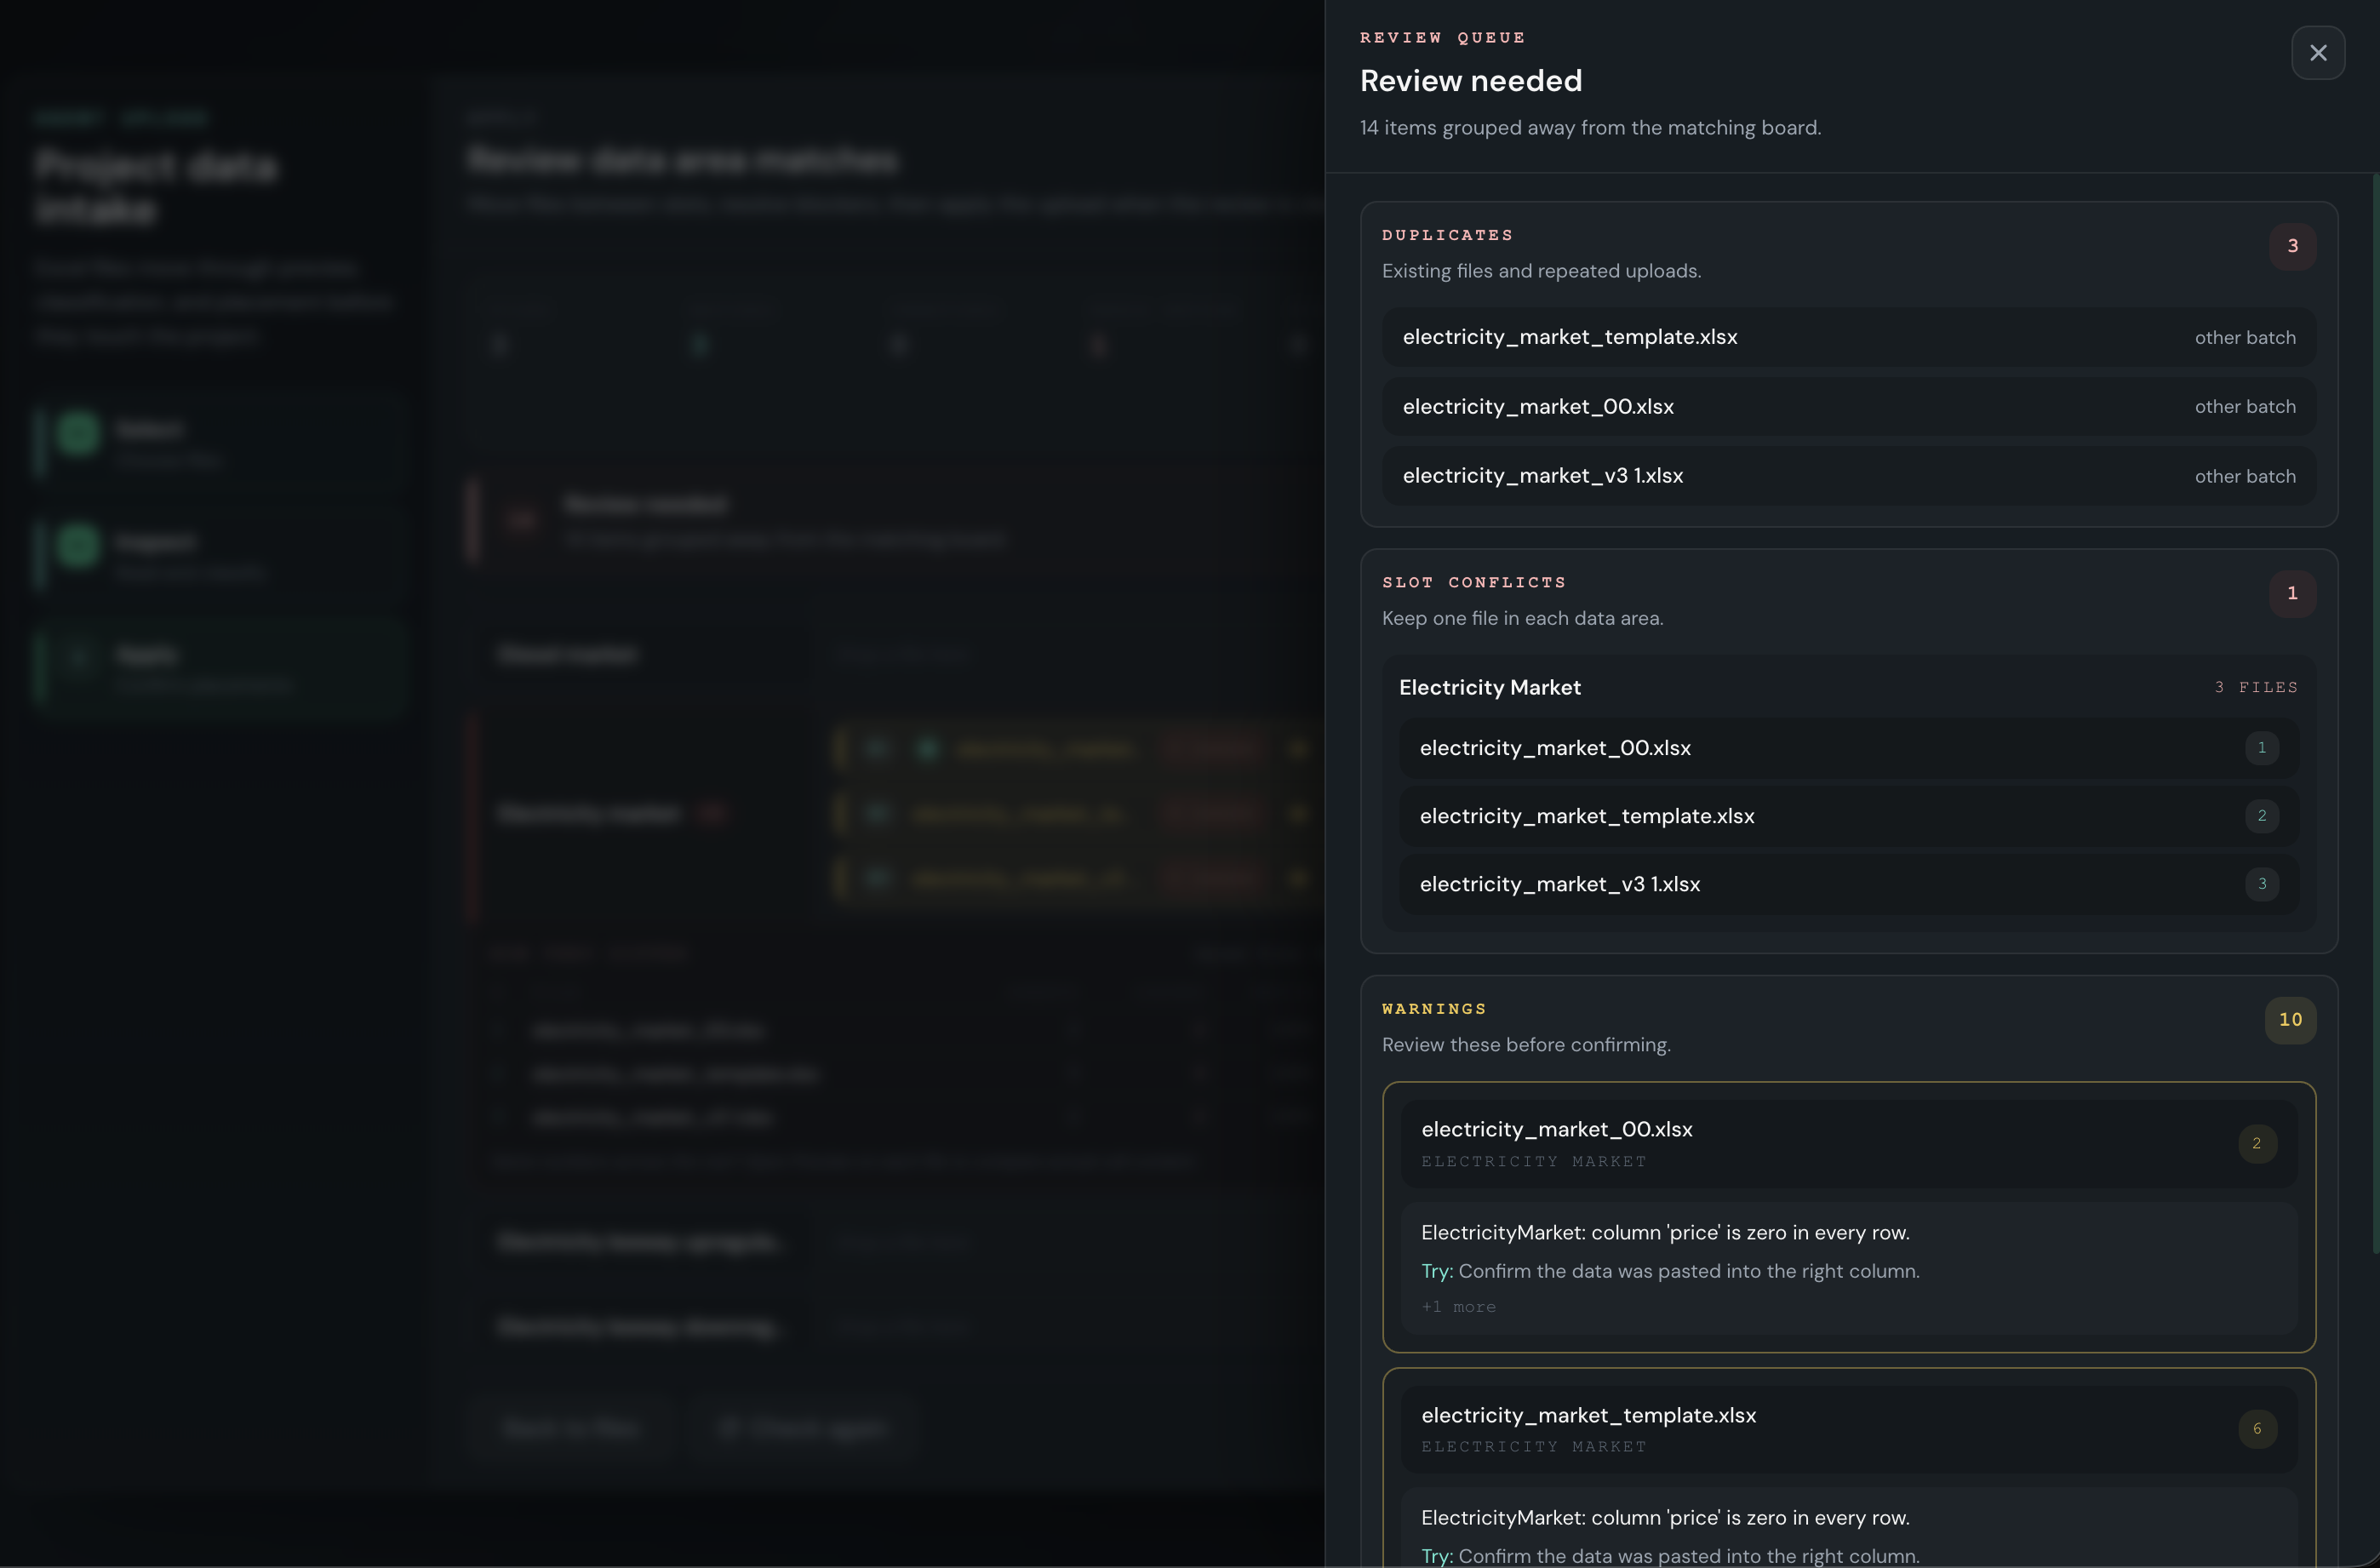
\includegraphics[width=0.9\linewidth]{Figures/chadi_review_queue.png}
  \caption{Review queue: duplicates, slot conflicts, and data-quality warnings to resolve.}
  \label{fig:impl-review}
\end{figure}

\subsection{Topology generation and parameter application}

The topology flow shows the assistant moving from explanation to proposal, with the
write path kept visible and approval-gated. Three responsibilities stay separate:
the agent interprets intent, the interface presents alternatives and pending
changes, and deterministic project state is updated only after confirmation
(Figures~\ref{fig:impl-topoexpl}--\ref{fig:impl-bulkchange}).

\begin{figure}[H]
  \centering
  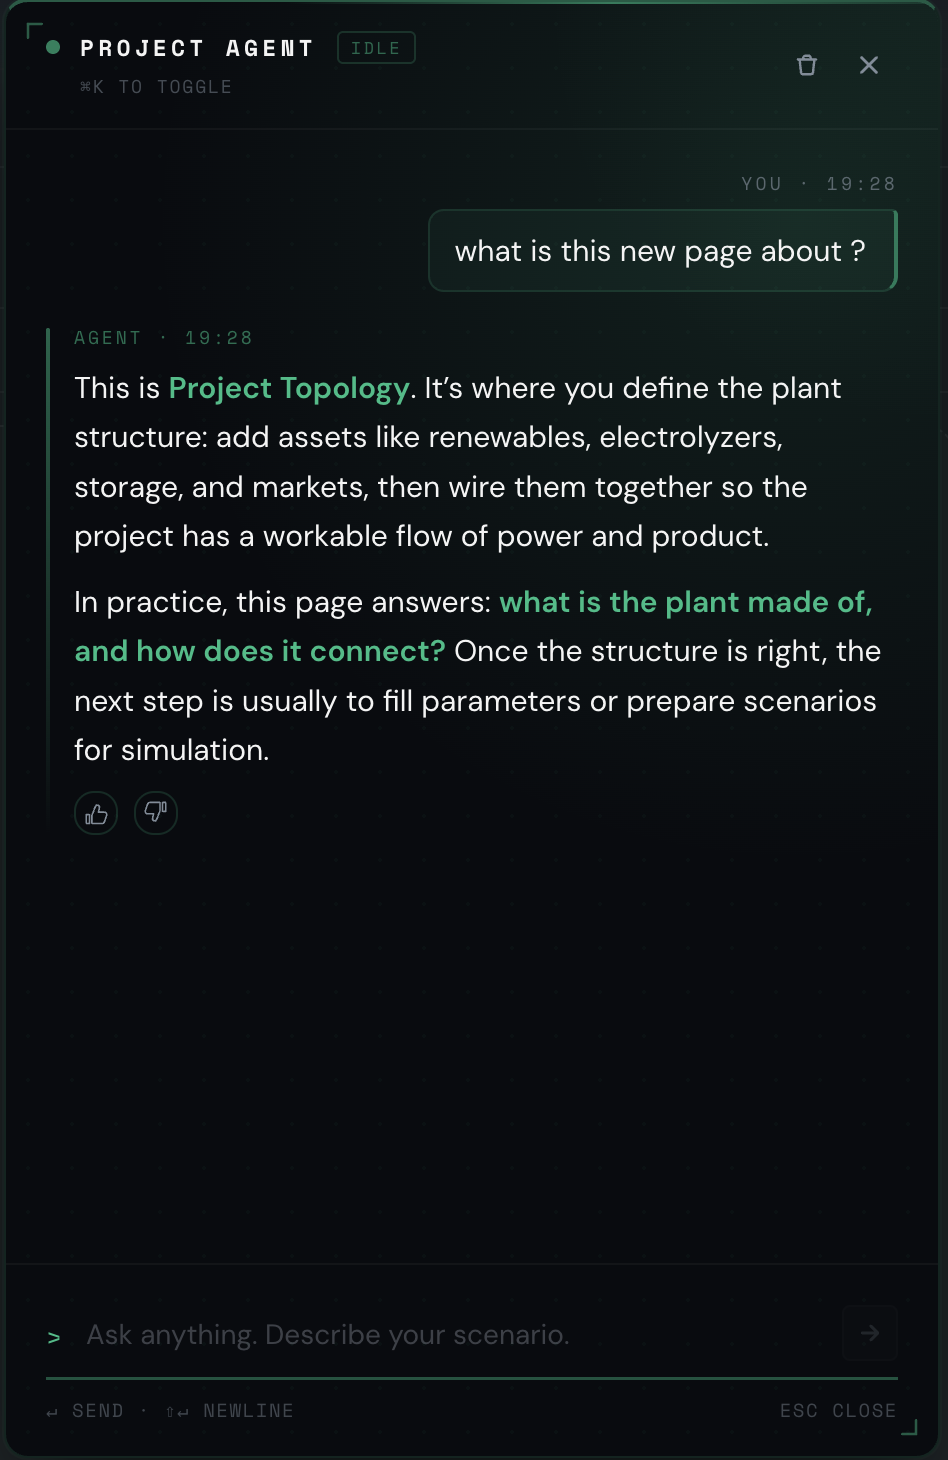
\includegraphics[width=0.48\linewidth]{Figures/chadi_topology_explanation.png}
  \caption{Topology explanation: the agent explains the graph before modifying it.}
  \label{fig:impl-topoexpl}
\end{figure}

\begin{figure}[H]
  \centering
  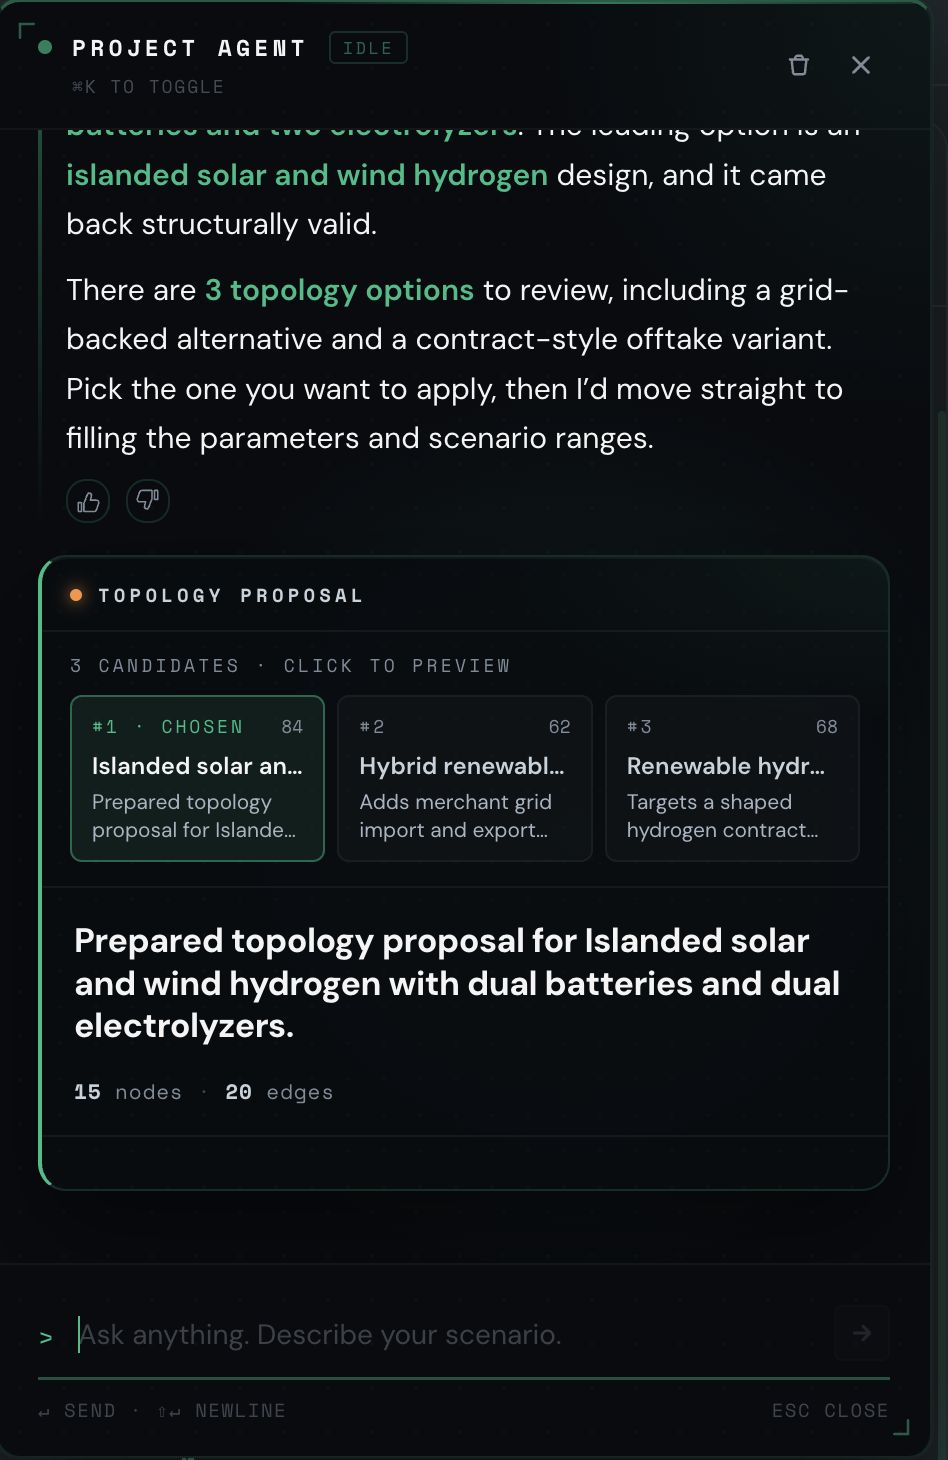
\includegraphics[width=0.48\linewidth]{Figures/chadi_topology_proposal.png}
  \caption{Topology proposal: candidate structures with a preferred option, for review.}
  \label{fig:impl-topoproposal}
\end{figure}

\begin{figure}[H]
  \centering
  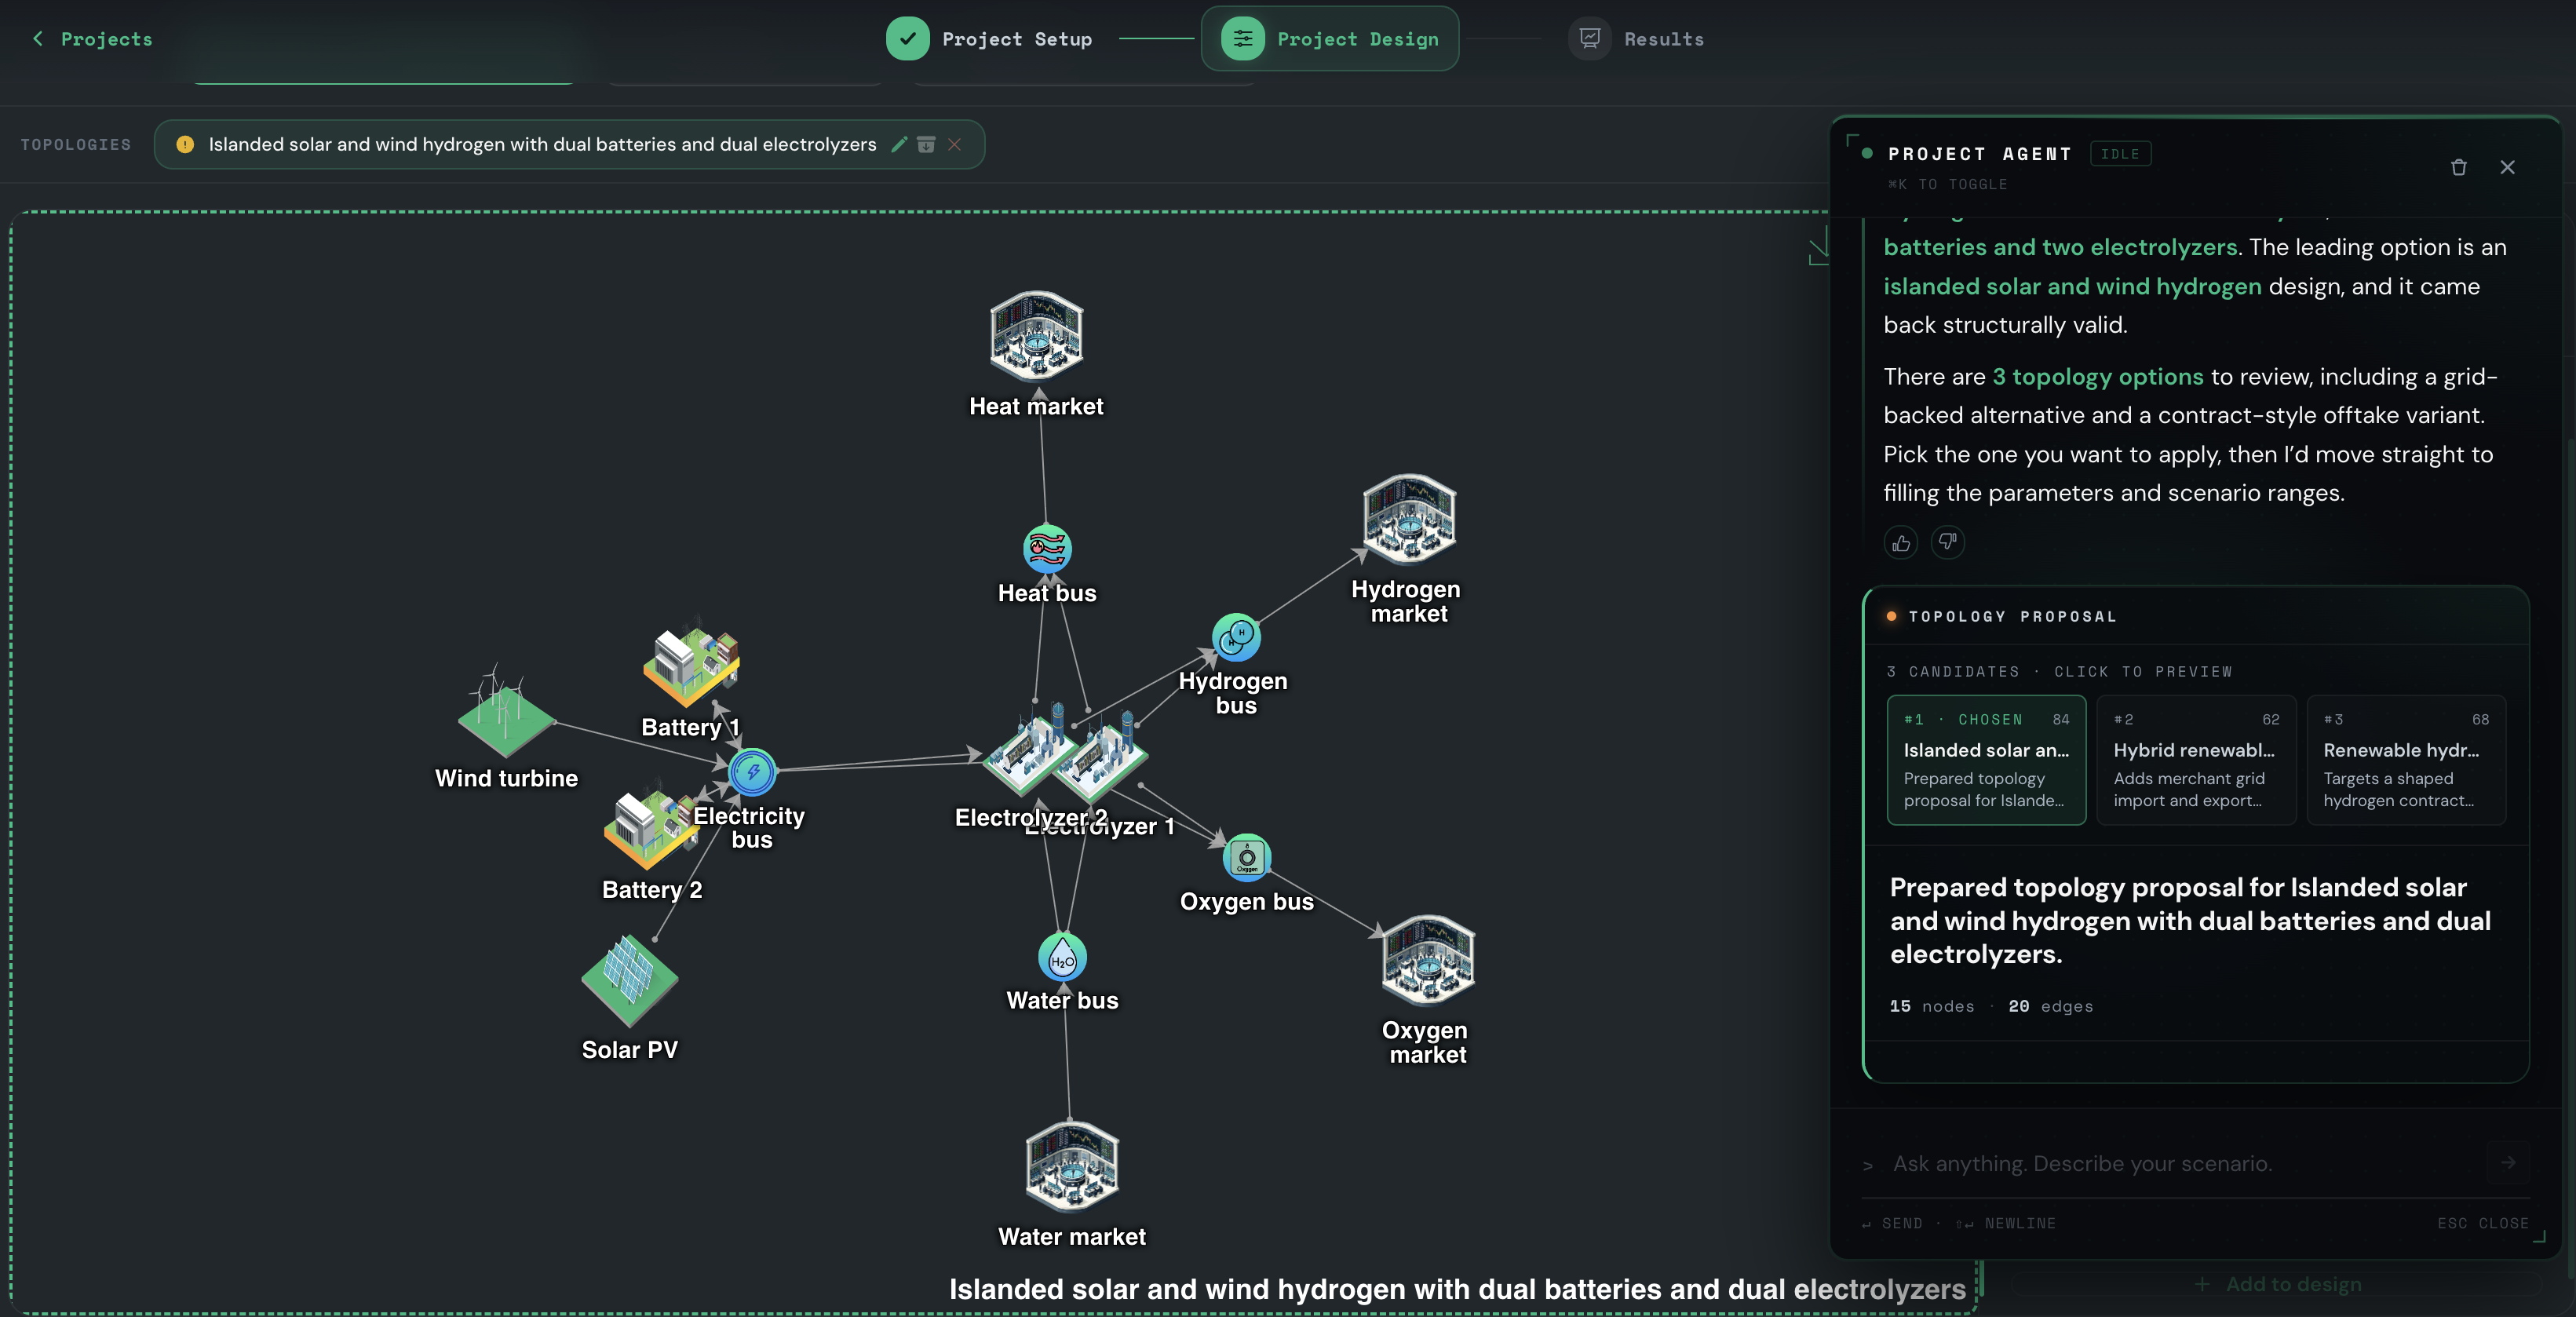
\includegraphics[width=0.95\linewidth]{Figures/chadi_generated_topology.png}
  \caption{Generated topology: the chosen structure appears on the canvas.}
  \label{fig:impl-gentopo}
\end{figure}

\begin{figure}[H]
  \centering
  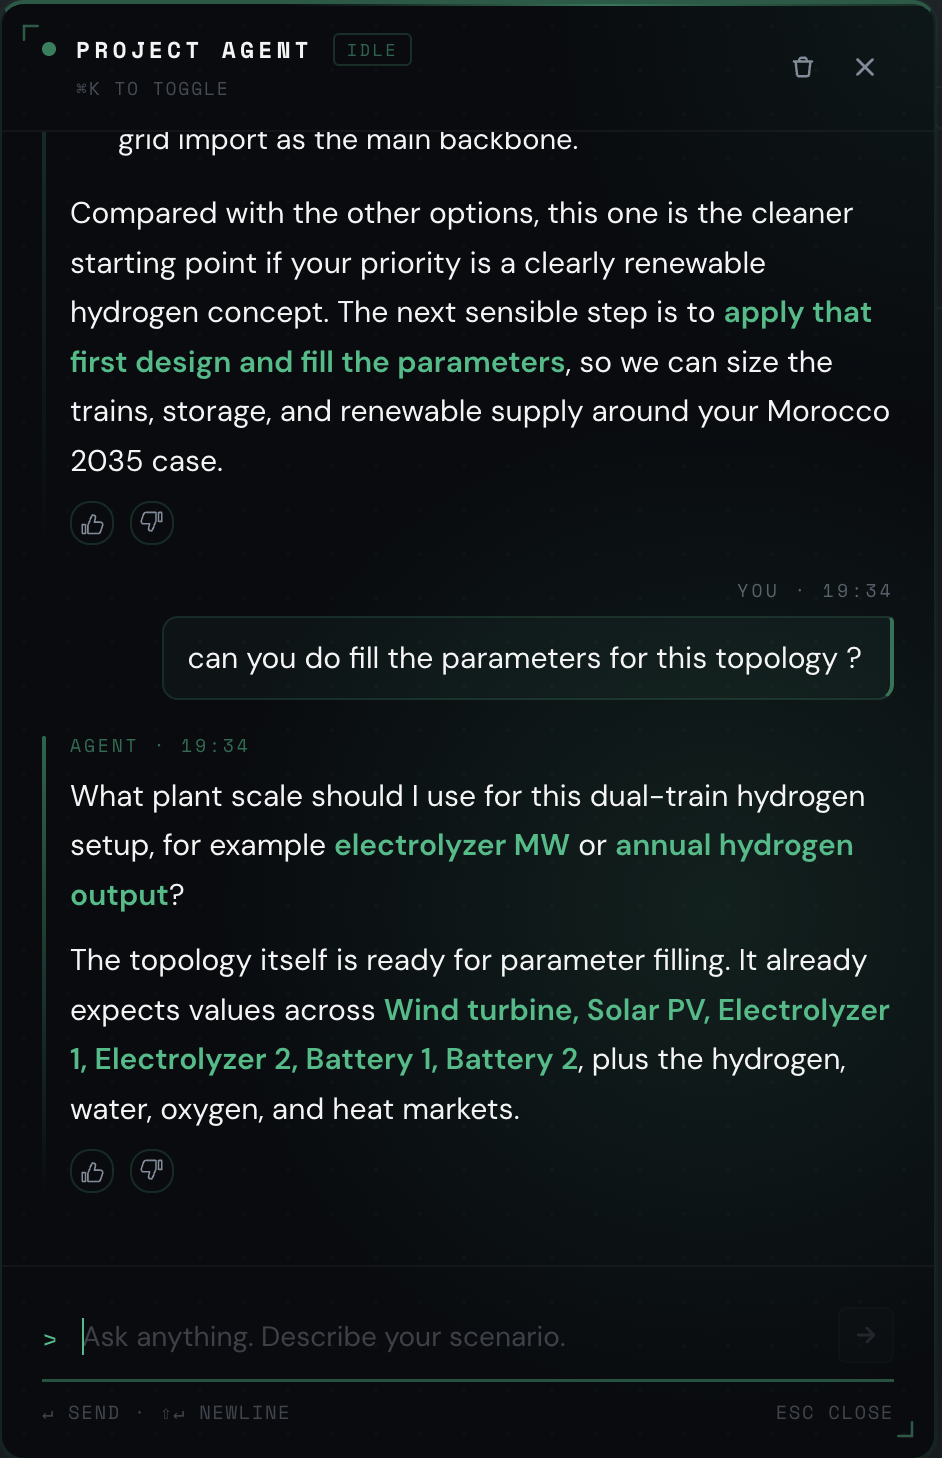
\includegraphics[width=0.48\linewidth]{Figures/chadi_missing_parameter.png}
  \caption{Missing parameter: the agent asks for a key sizing input rather than inventing it.}
  \label{fig:impl-missingparam}
\end{figure}

\begin{figure}[H]
  \centering
  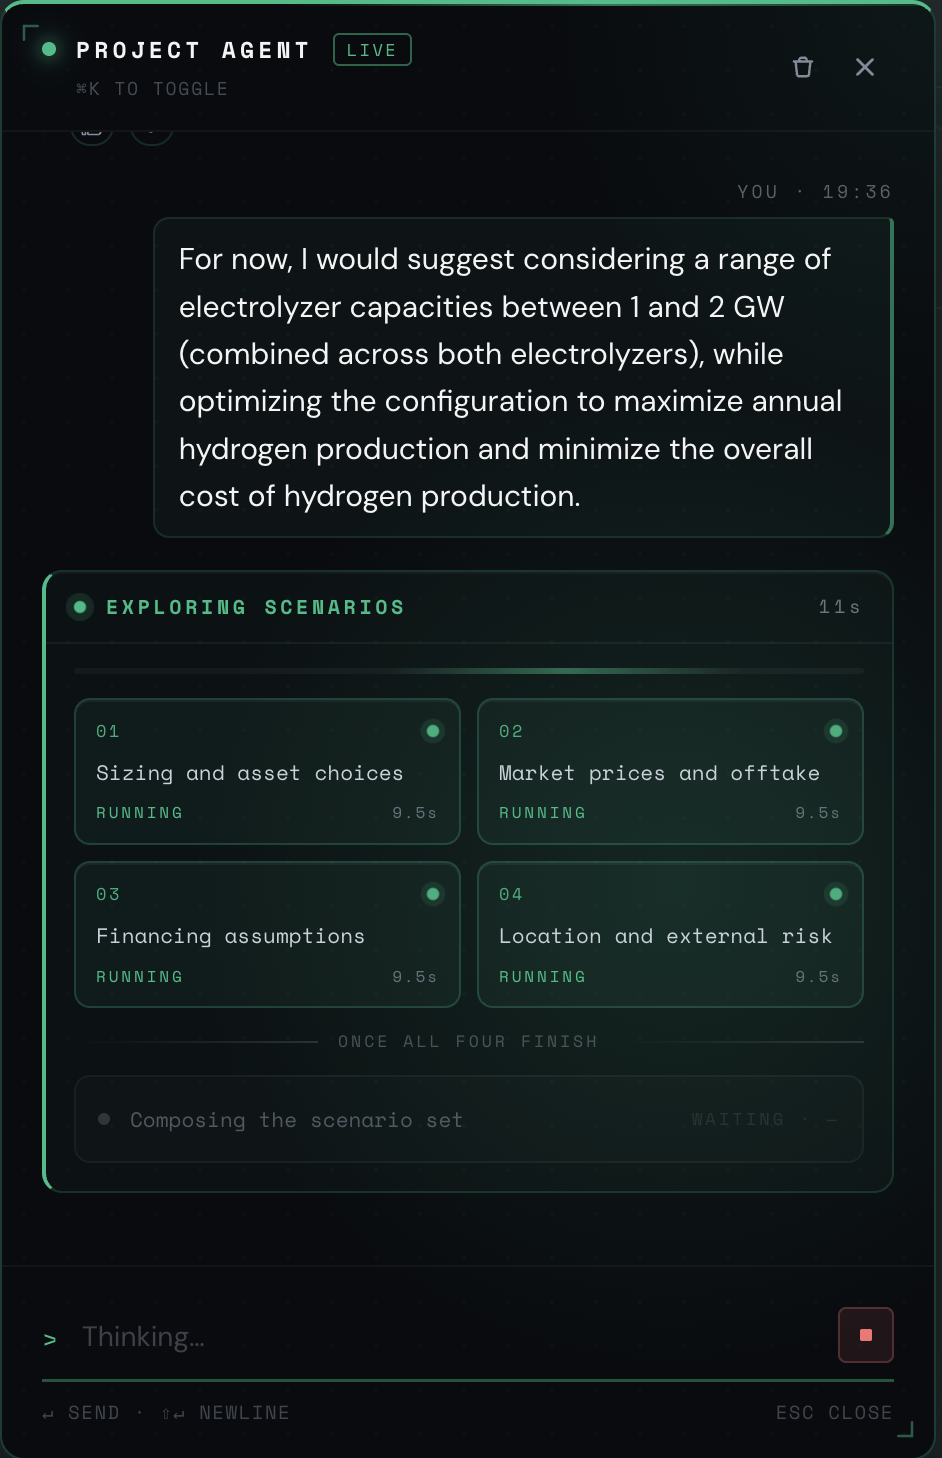
\includegraphics[width=0.48\linewidth]{Figures/chadi_scenario_cards.png}
  \caption{Scenario cards: study directions turned into a manageable sweep.}
  \label{fig:impl-scenariocards}
\end{figure}

\begin{figure}[H]
  \centering
  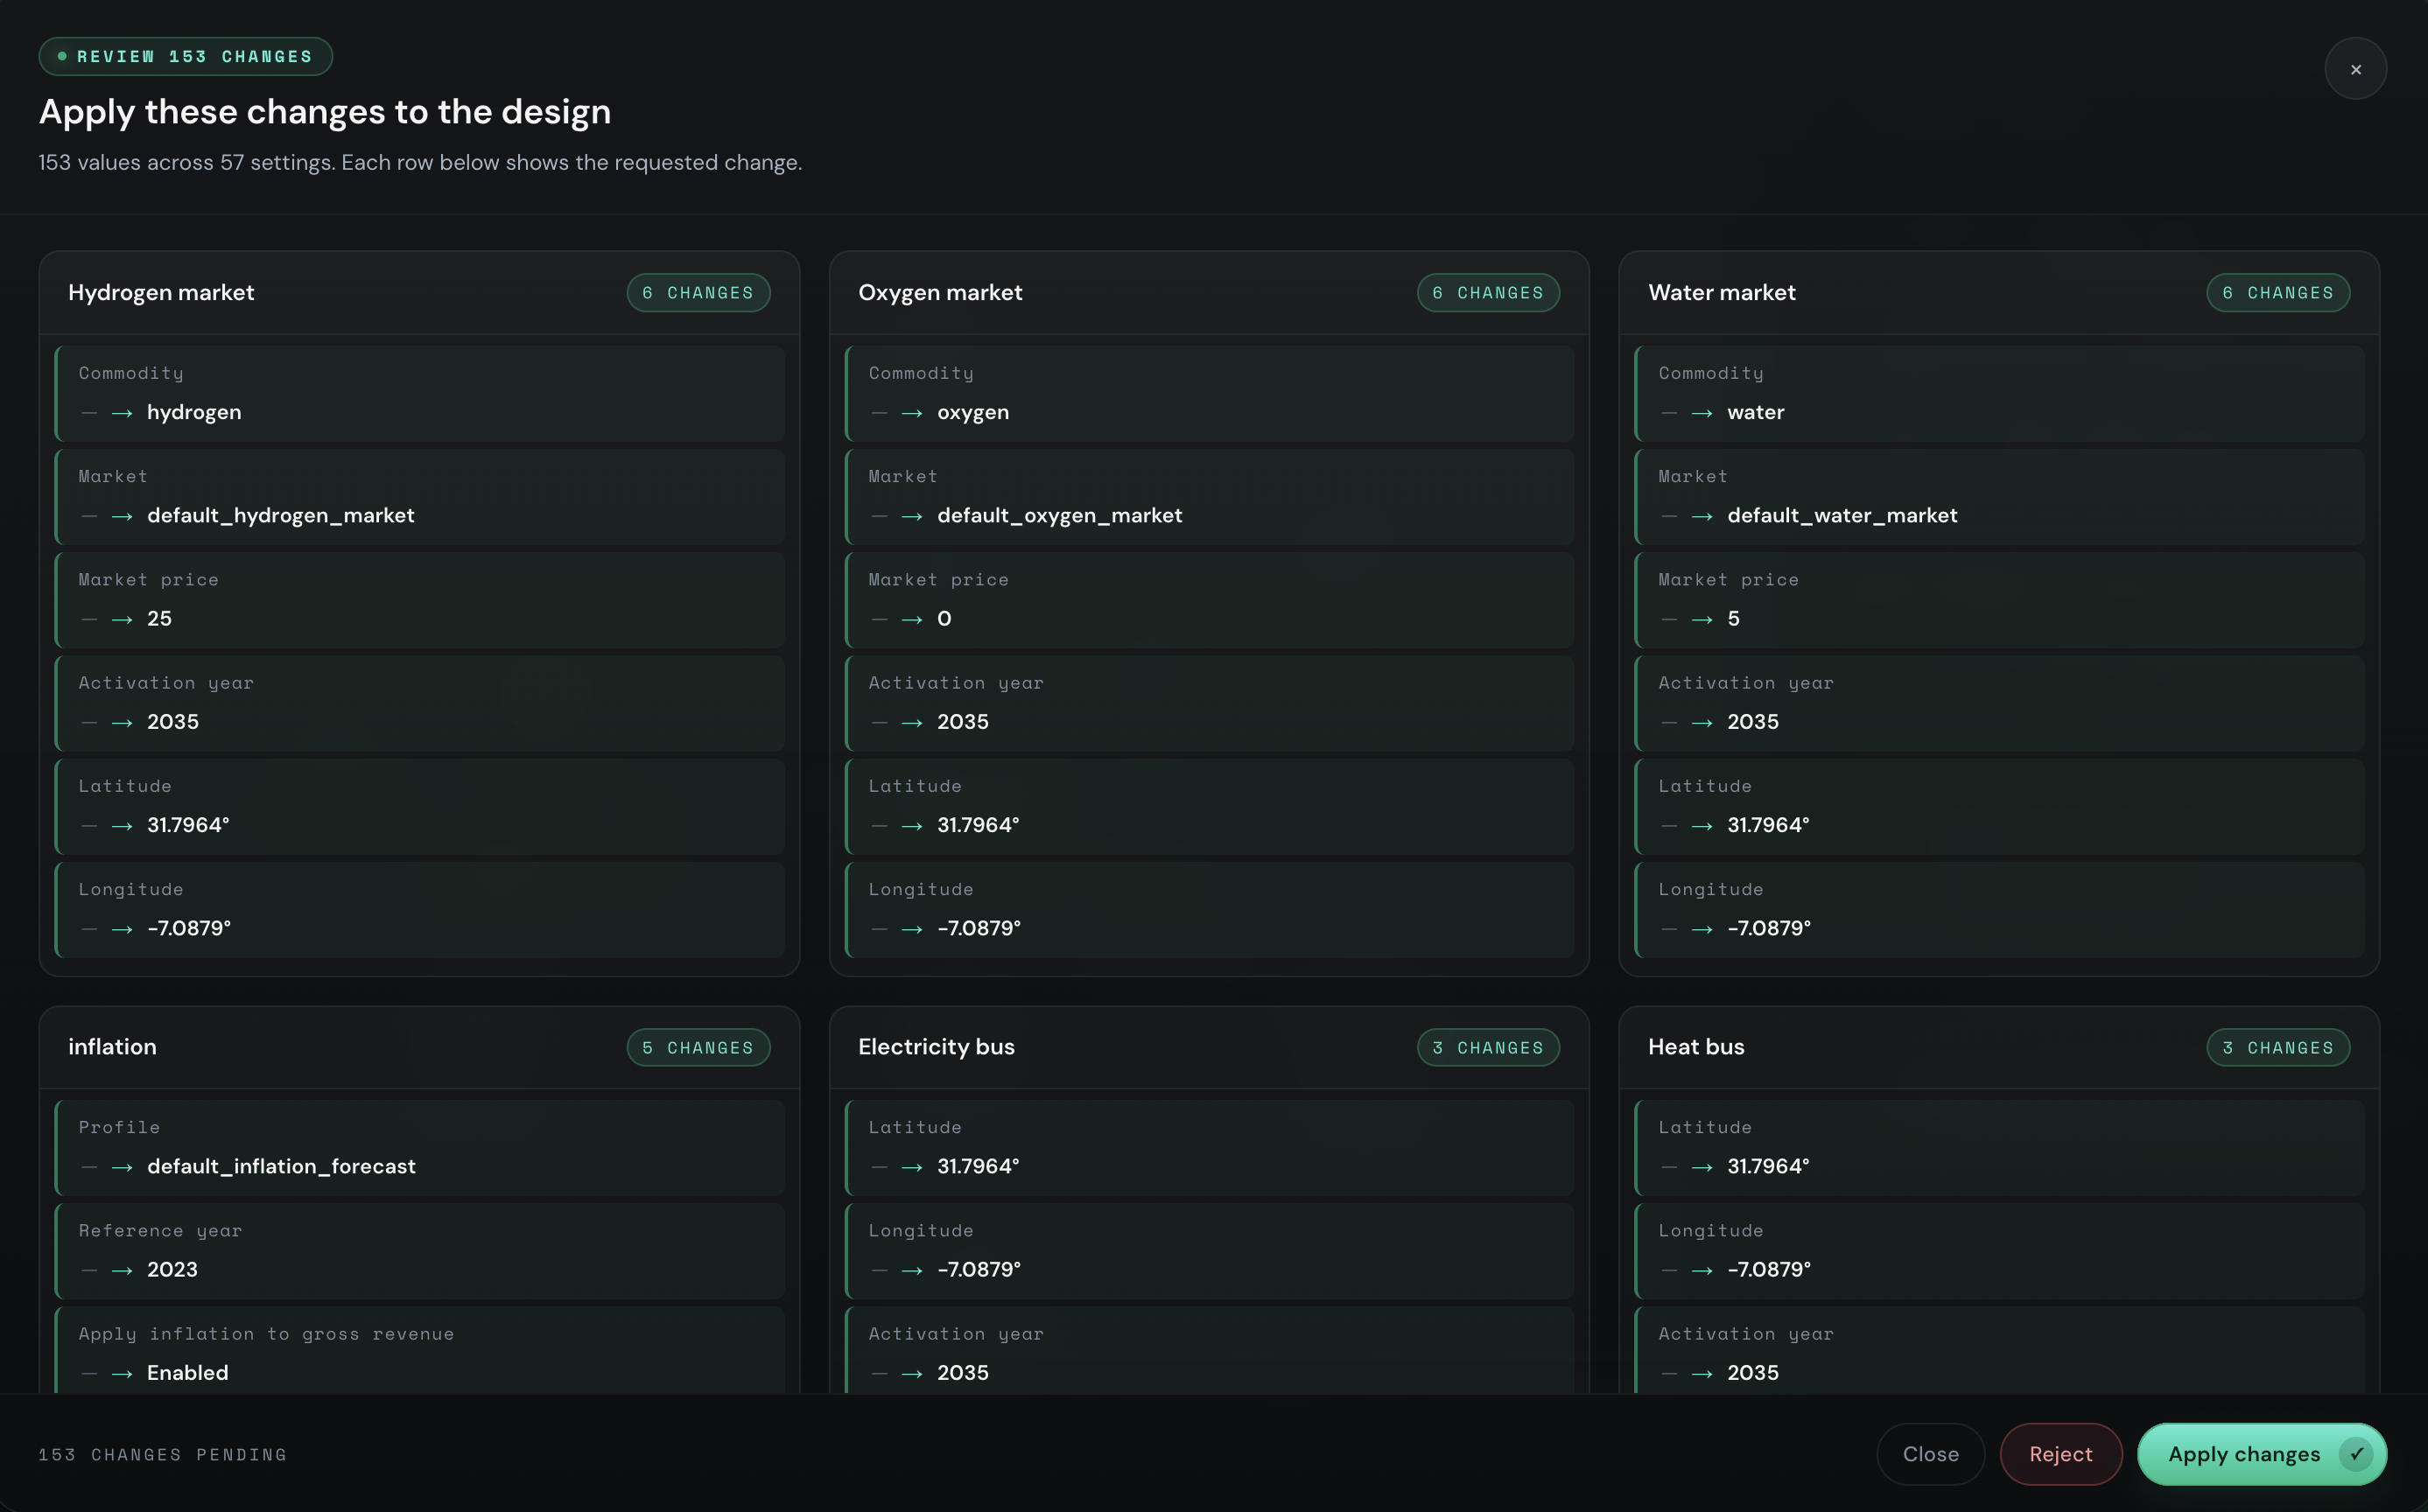
\includegraphics[width=0.9\linewidth]{Figures/chadi_bulk_change.png}
  \caption{Bulk change review: proposed values grouped by entity, auditable before applying.}
  \label{fig:impl-bulkchange}
\end{figure}

\subsection{Result exploration and interpretation}
\label{sec:impl-results}

The final stage of the journey is result exploration and
interpretation. Once a grid search has completed, its population of
simulations is explored through an interactive results view built as a set of
components over the deterministic outputs, organized so that a user moves from
comparing a whole population of runs, to reading one run in depth, to asking for an
explanation of exactly what is on screen.

Runs are first browsed and managed in a results library, with live status, search,
download, and cancellation (Figure~\ref{fig:impl-library}). The chart view is the
analytical core: a scatter with selectable axes plots one point per simulation and
makes trade-offs and standout runs immediately visible, with dense tables for exact
comparison (Figure~\ref{fig:impl-scatter}). Selecting a run opens a six-panel
operational dashboard that tells that run's operational money story, governed by a
time-filter sidebar (Figure~\ref{fig:impl-dashboard}). The financial output is
rendered as a grouped, expandable discounted-cash-flow table with drill-down to
per-asset and per-market components, amortization and debt groups, reconciliation,
payback highlighting, and hover-for-exact-figure (Figure~\ref{fig:impl-dcf}). From
any chart or run, the analyst can ask the interpreter to explain what is shown; the
agent streams a plain-language narration and a set of insight cards, citing only
figures read from the deterministic output, and can embed the chart it refers to
(Figure~\ref{fig:impl-interp}); further interpretation examples are shown in
Figure~\ref{fig:impl-interp-examples}.

\begin{figure}[H]
  \centering
  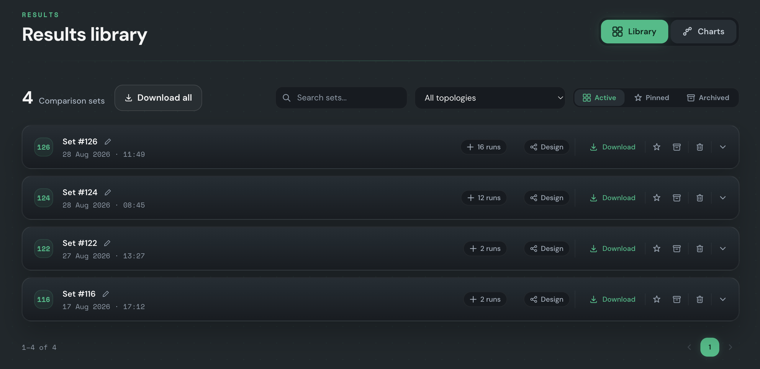
\includegraphics[width=0.95\linewidth]{Figures/impl_library.png}
  \caption{The results library: run management with status, search, and per-run actions.}
  \label{fig:impl-library}
\end{figure}

\begin{figure}[H]
  \centering
  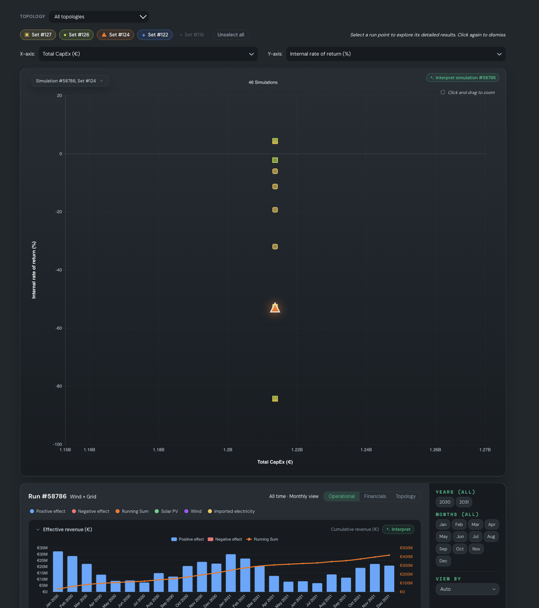
\includegraphics[width=0.72\linewidth]{Figures/impl_scatter.png}
  \caption{Interactive results exploration: a scatter with selectable axes and interpret-on-demand.}
  \label{fig:impl-scatter}
\end{figure}

\begin{figure}[H]
  \centering
  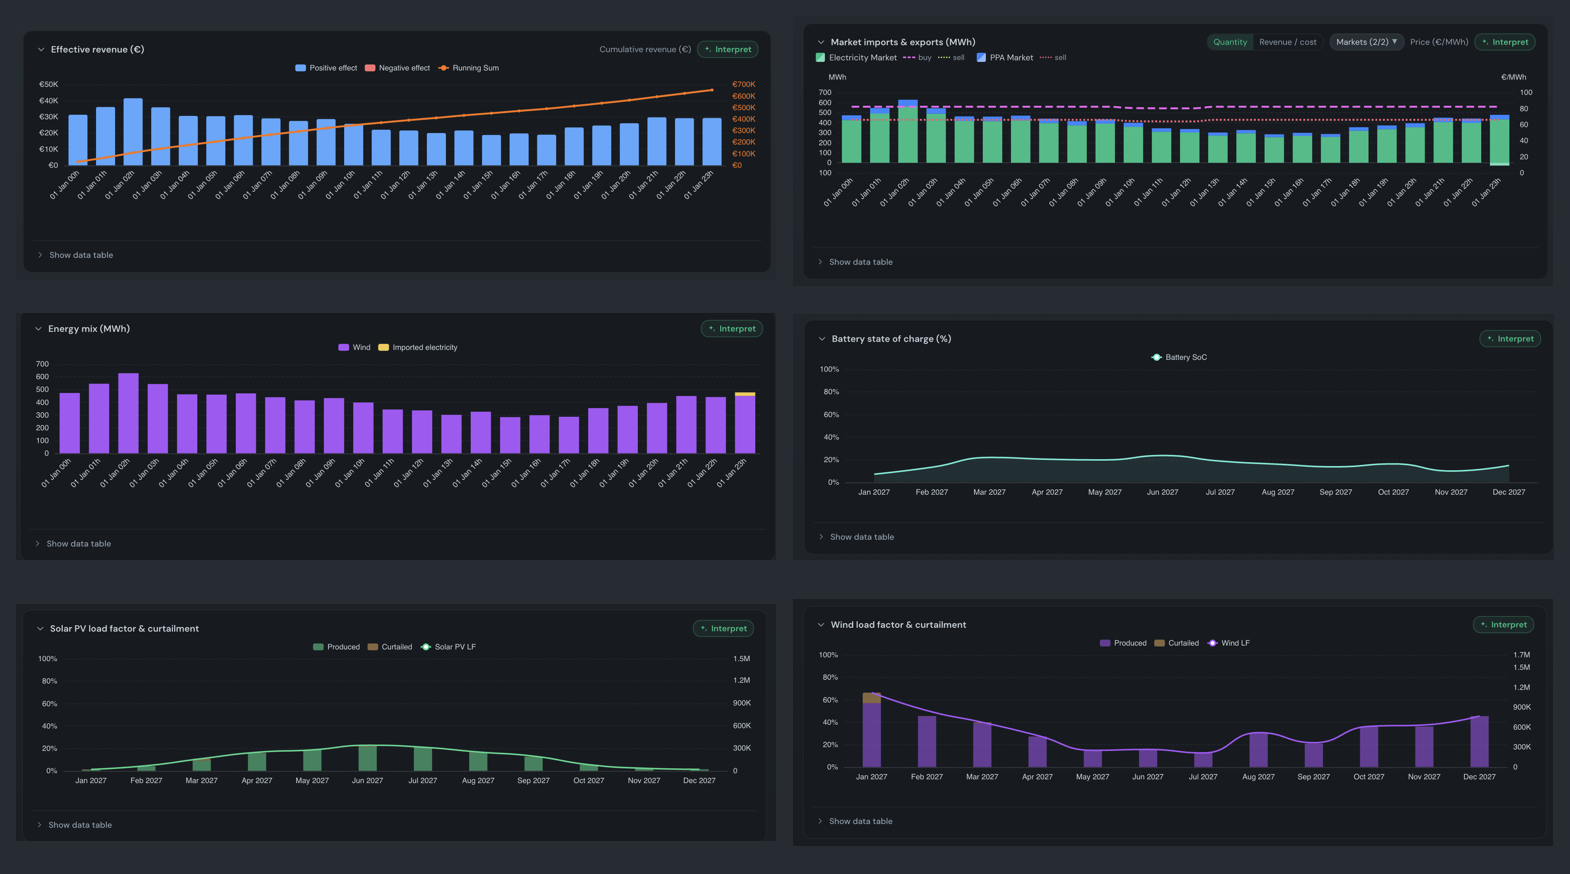
\includegraphics[width=\linewidth]{Figures/impl_dashboard.png}
  \caption{The per-run operational dashboard: the six-panel operational money story.}
  \label{fig:impl-dashboard}
\end{figure}

\begin{figure}[H]
  \centering
  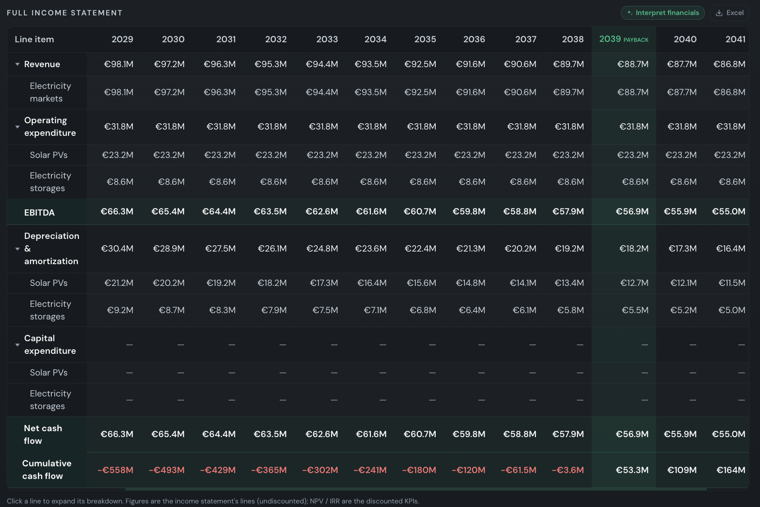
\includegraphics[width=0.92\linewidth]{Figures/impl_dcf.png}
  \caption{Navigable discounted-cash-flow table with drill-down and payback highlighting.}
  \label{fig:impl-dcf}
\end{figure}

\begin{figure}[H]
  \centering
  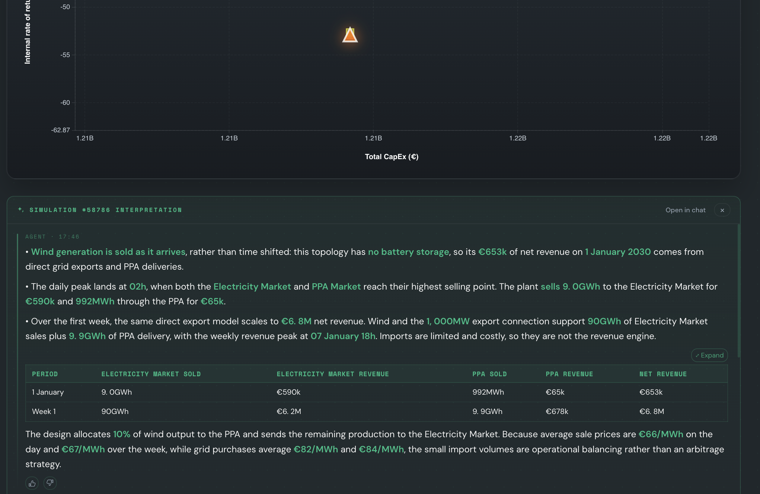
\includegraphics[width=0.8\linewidth]{Figures/impl_interp.png}
  \caption{Grounded, streamed interpretation of a run, with insight cards and the referenced chart.}
  \label{fig:impl-interp}
\end{figure}


\begin{figure}[H]
  \centering
  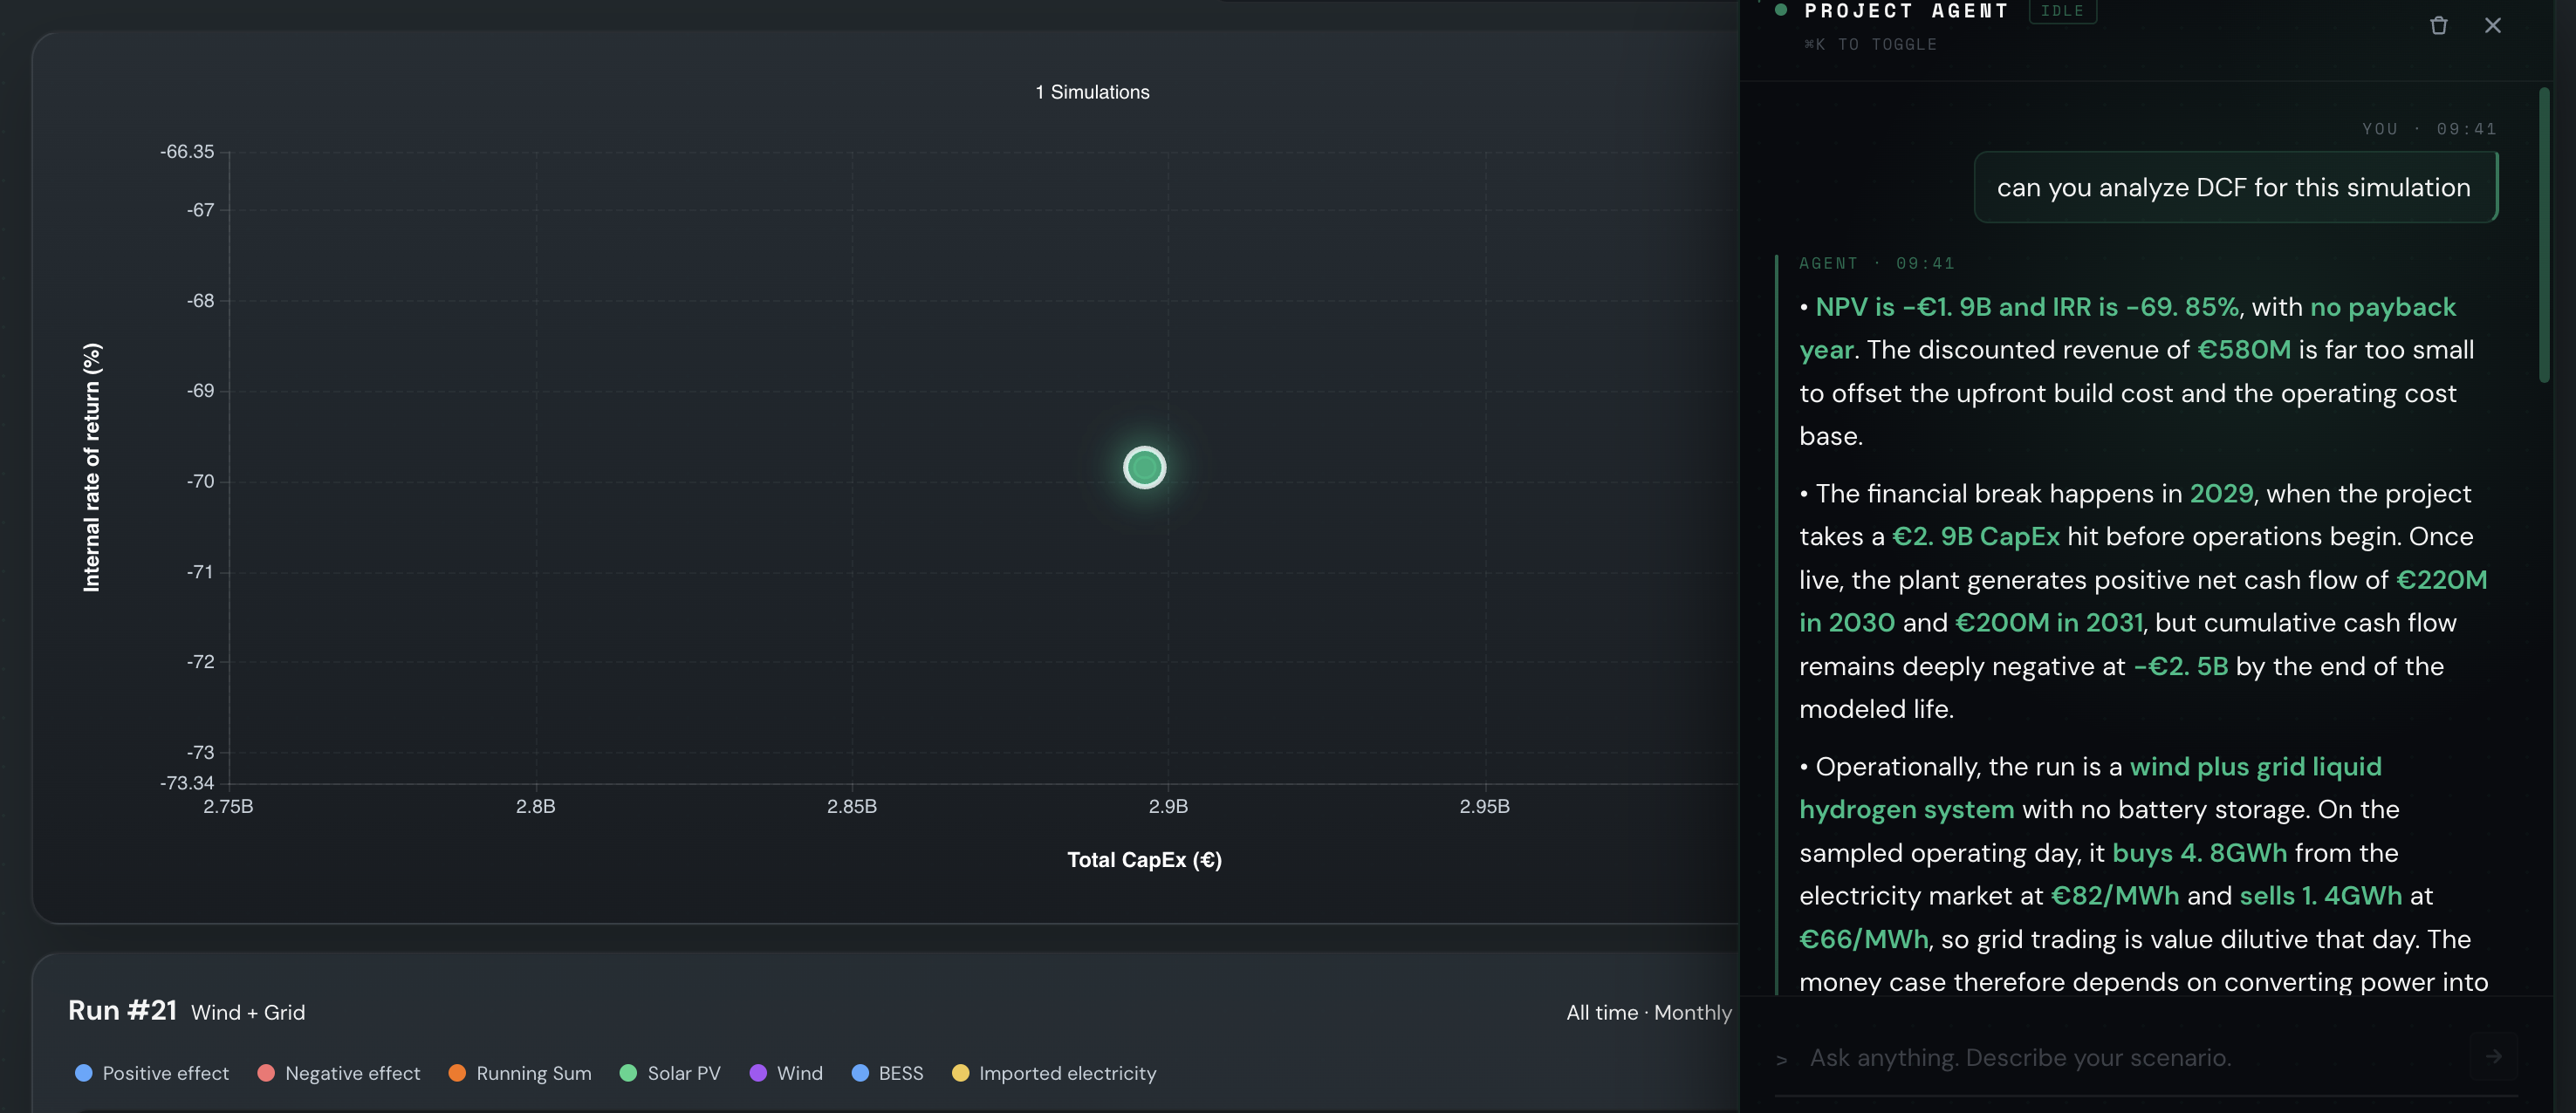
\includegraphics[width=0.64\linewidth]{Figures/image (19).png}\\[0.15cm]
  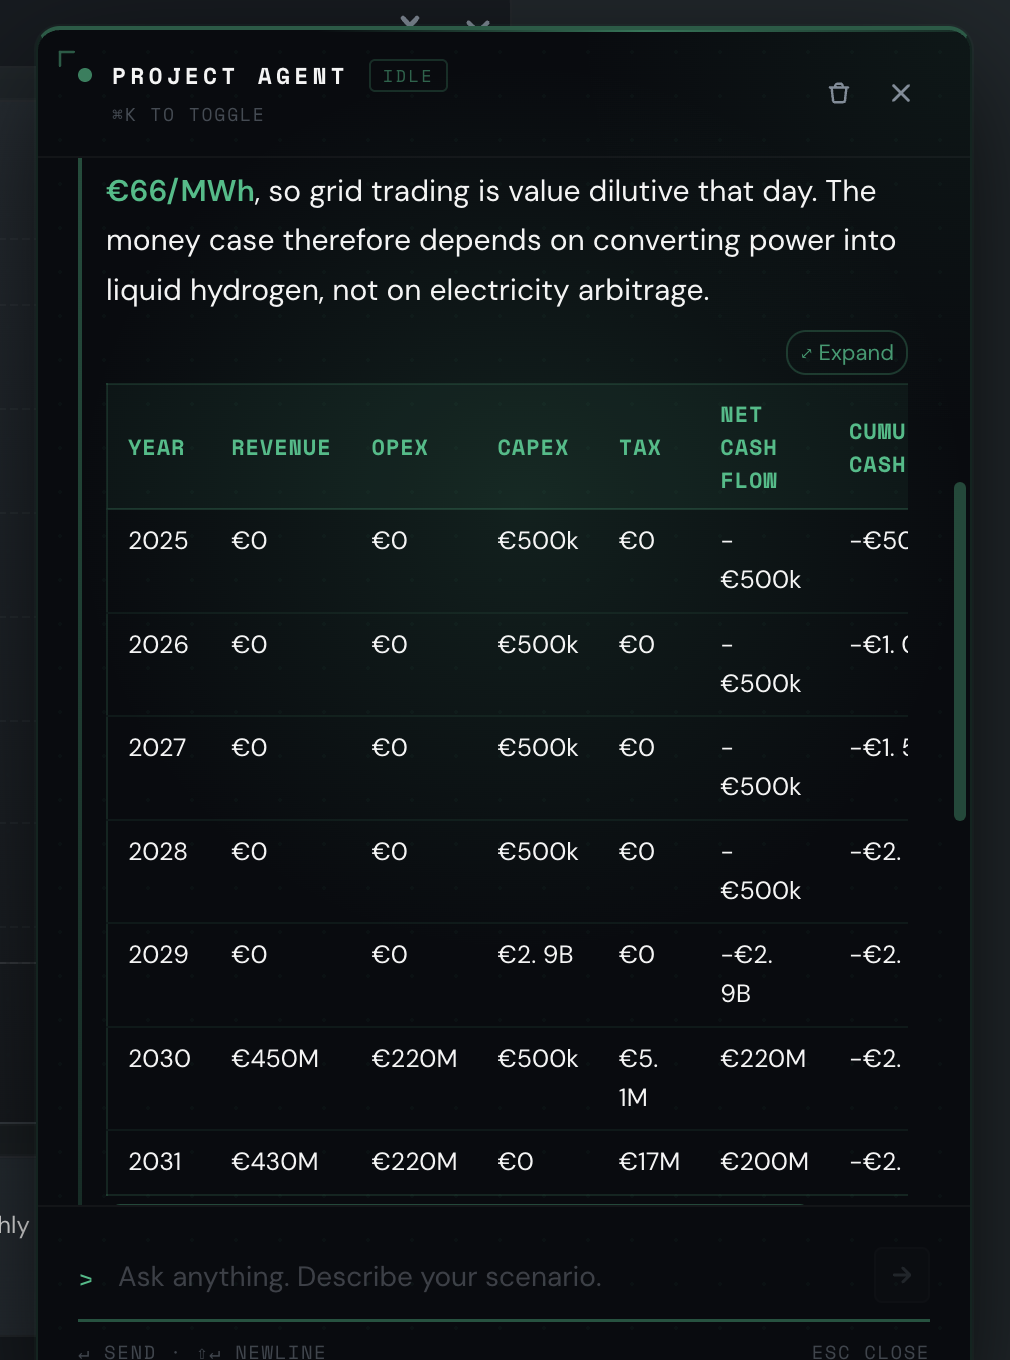
\includegraphics[width=0.3\linewidth]{Figures/image (20).png}
  \hspace{0.04\linewidth}
  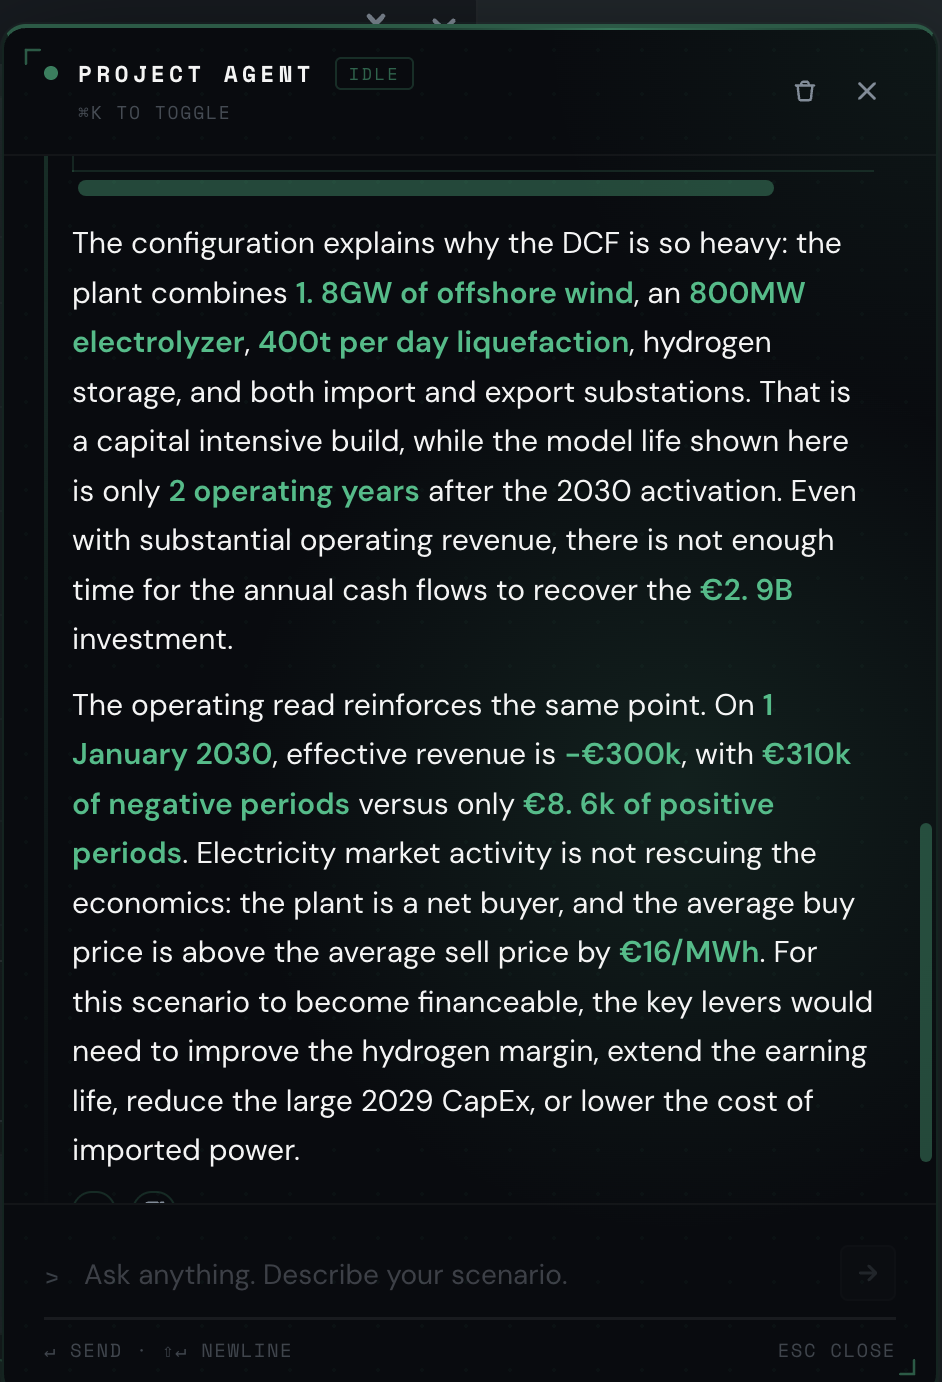
\includegraphics[width=0.3\linewidth]{Figures/image (22).png}
  \caption{Interpretation examples: a run analyzed beside its scatter (top), and,
    within the chat, an embedded discounted-cash-flow table and a grounded
    narrative citing deterministic figures (bottom).}
  \label{fig:impl-interp-examples}
\end{figure}

\newpage

In the delivered system these capabilities are shipped, not prototypes. The
interpreter runs on the separate agent runtime and is exposed as a single Director
tool (Figure~\ref{fig:impl-interp-arch}), so a user reaches it from the same chat
that drives the rest of the workflow; each explanation is a fresh, grounded turn
streamed token by token into an inline block beneath the exact chart it describes.
The scatter, the operational dashboard, the discounted-cash-flow table, and the
interpreter all read the \textbf{same pure, unit-tested analytics}, so the figures a
written explanation cites cannot differ from the figures a chart plots. The result
is that a non-specialist can move from a population of runs, to one run's
operational and financial story, to a grounded answer about what it means, without
leaving the results page and without any number originating from the model.

\begin{figure}[H]
  \centering
  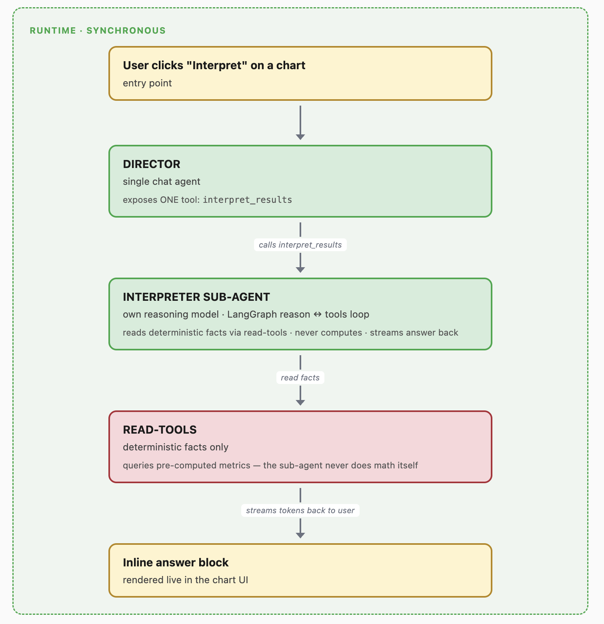
\includegraphics[width=0.6\linewidth]{Figures/impl_interp_arch.png}
  \caption{The implemented interpreter architecture: the Director exposes it as one read-only reason-and-tools loop.}
  \label{fig:impl-interp-arch}
\end{figure}

\section{Platform and operations implementation}
\label{sec:impl-ops}

The analytical experience runs on the restored platform. This section reports the
surrounding platform and operations work, from enterprise access to observability.

\subsection{Enterprise access verification}

Access is routed through the enterprise identity flow: the sign-in path redirects
users to the organization-managed verification screen before returning
authenticated traffic to the application (Figure~\ref{fig:impl-okta}). This confirms
that authentication was moved out of the product runtime and into the
organization-controlled identity path.

\begin{figure}[H]
  \centering
  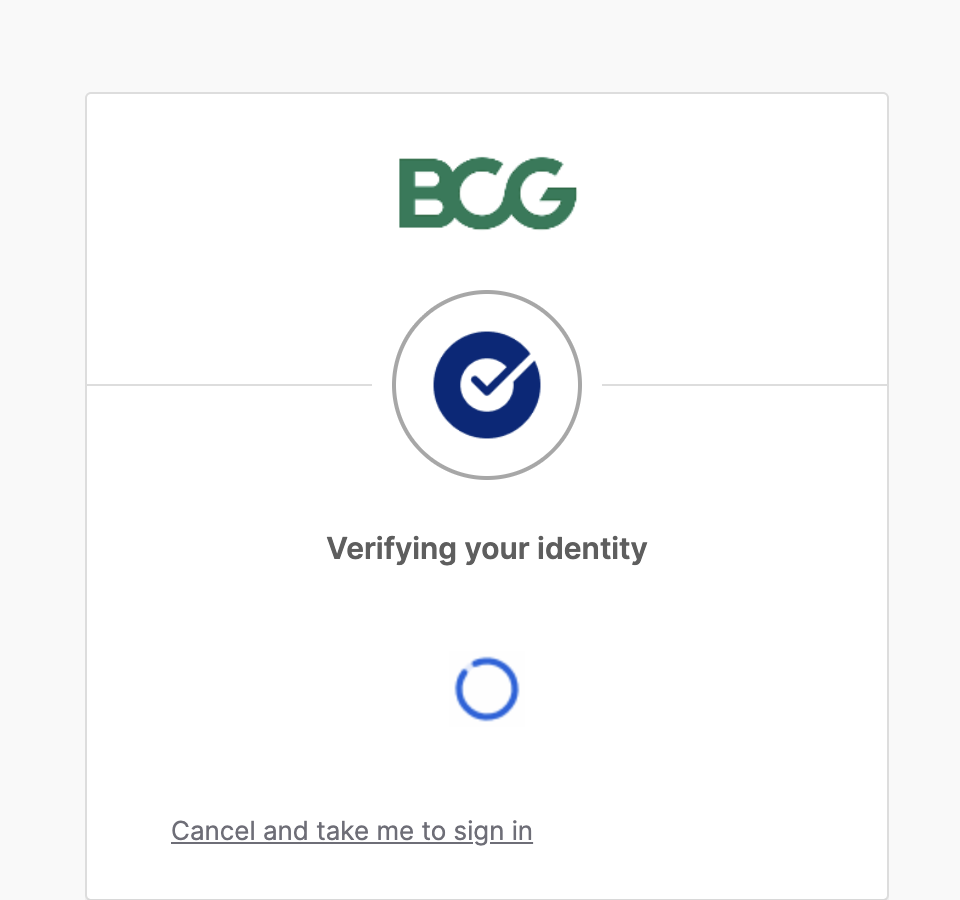
\includegraphics[width=0.5\linewidth]{Figures/chadi_okta.png}
  \caption{Enterprise identity verification: sign-in before reaching the application.}
  \label{fig:impl-okta}
\end{figure}

\subsection{Deployment and infrastructure delivery}

The restored delivery chain shows that the product can move from a code change to a
controlled deployment again: application changes pass through continuous-integration
workflows and infrastructure changes are applied through infrastructure-as-code
(Figures~\ref{fig:impl-circleci} and~\ref{fig:impl-terraform}).

\begin{figure}[H]
  \centering
  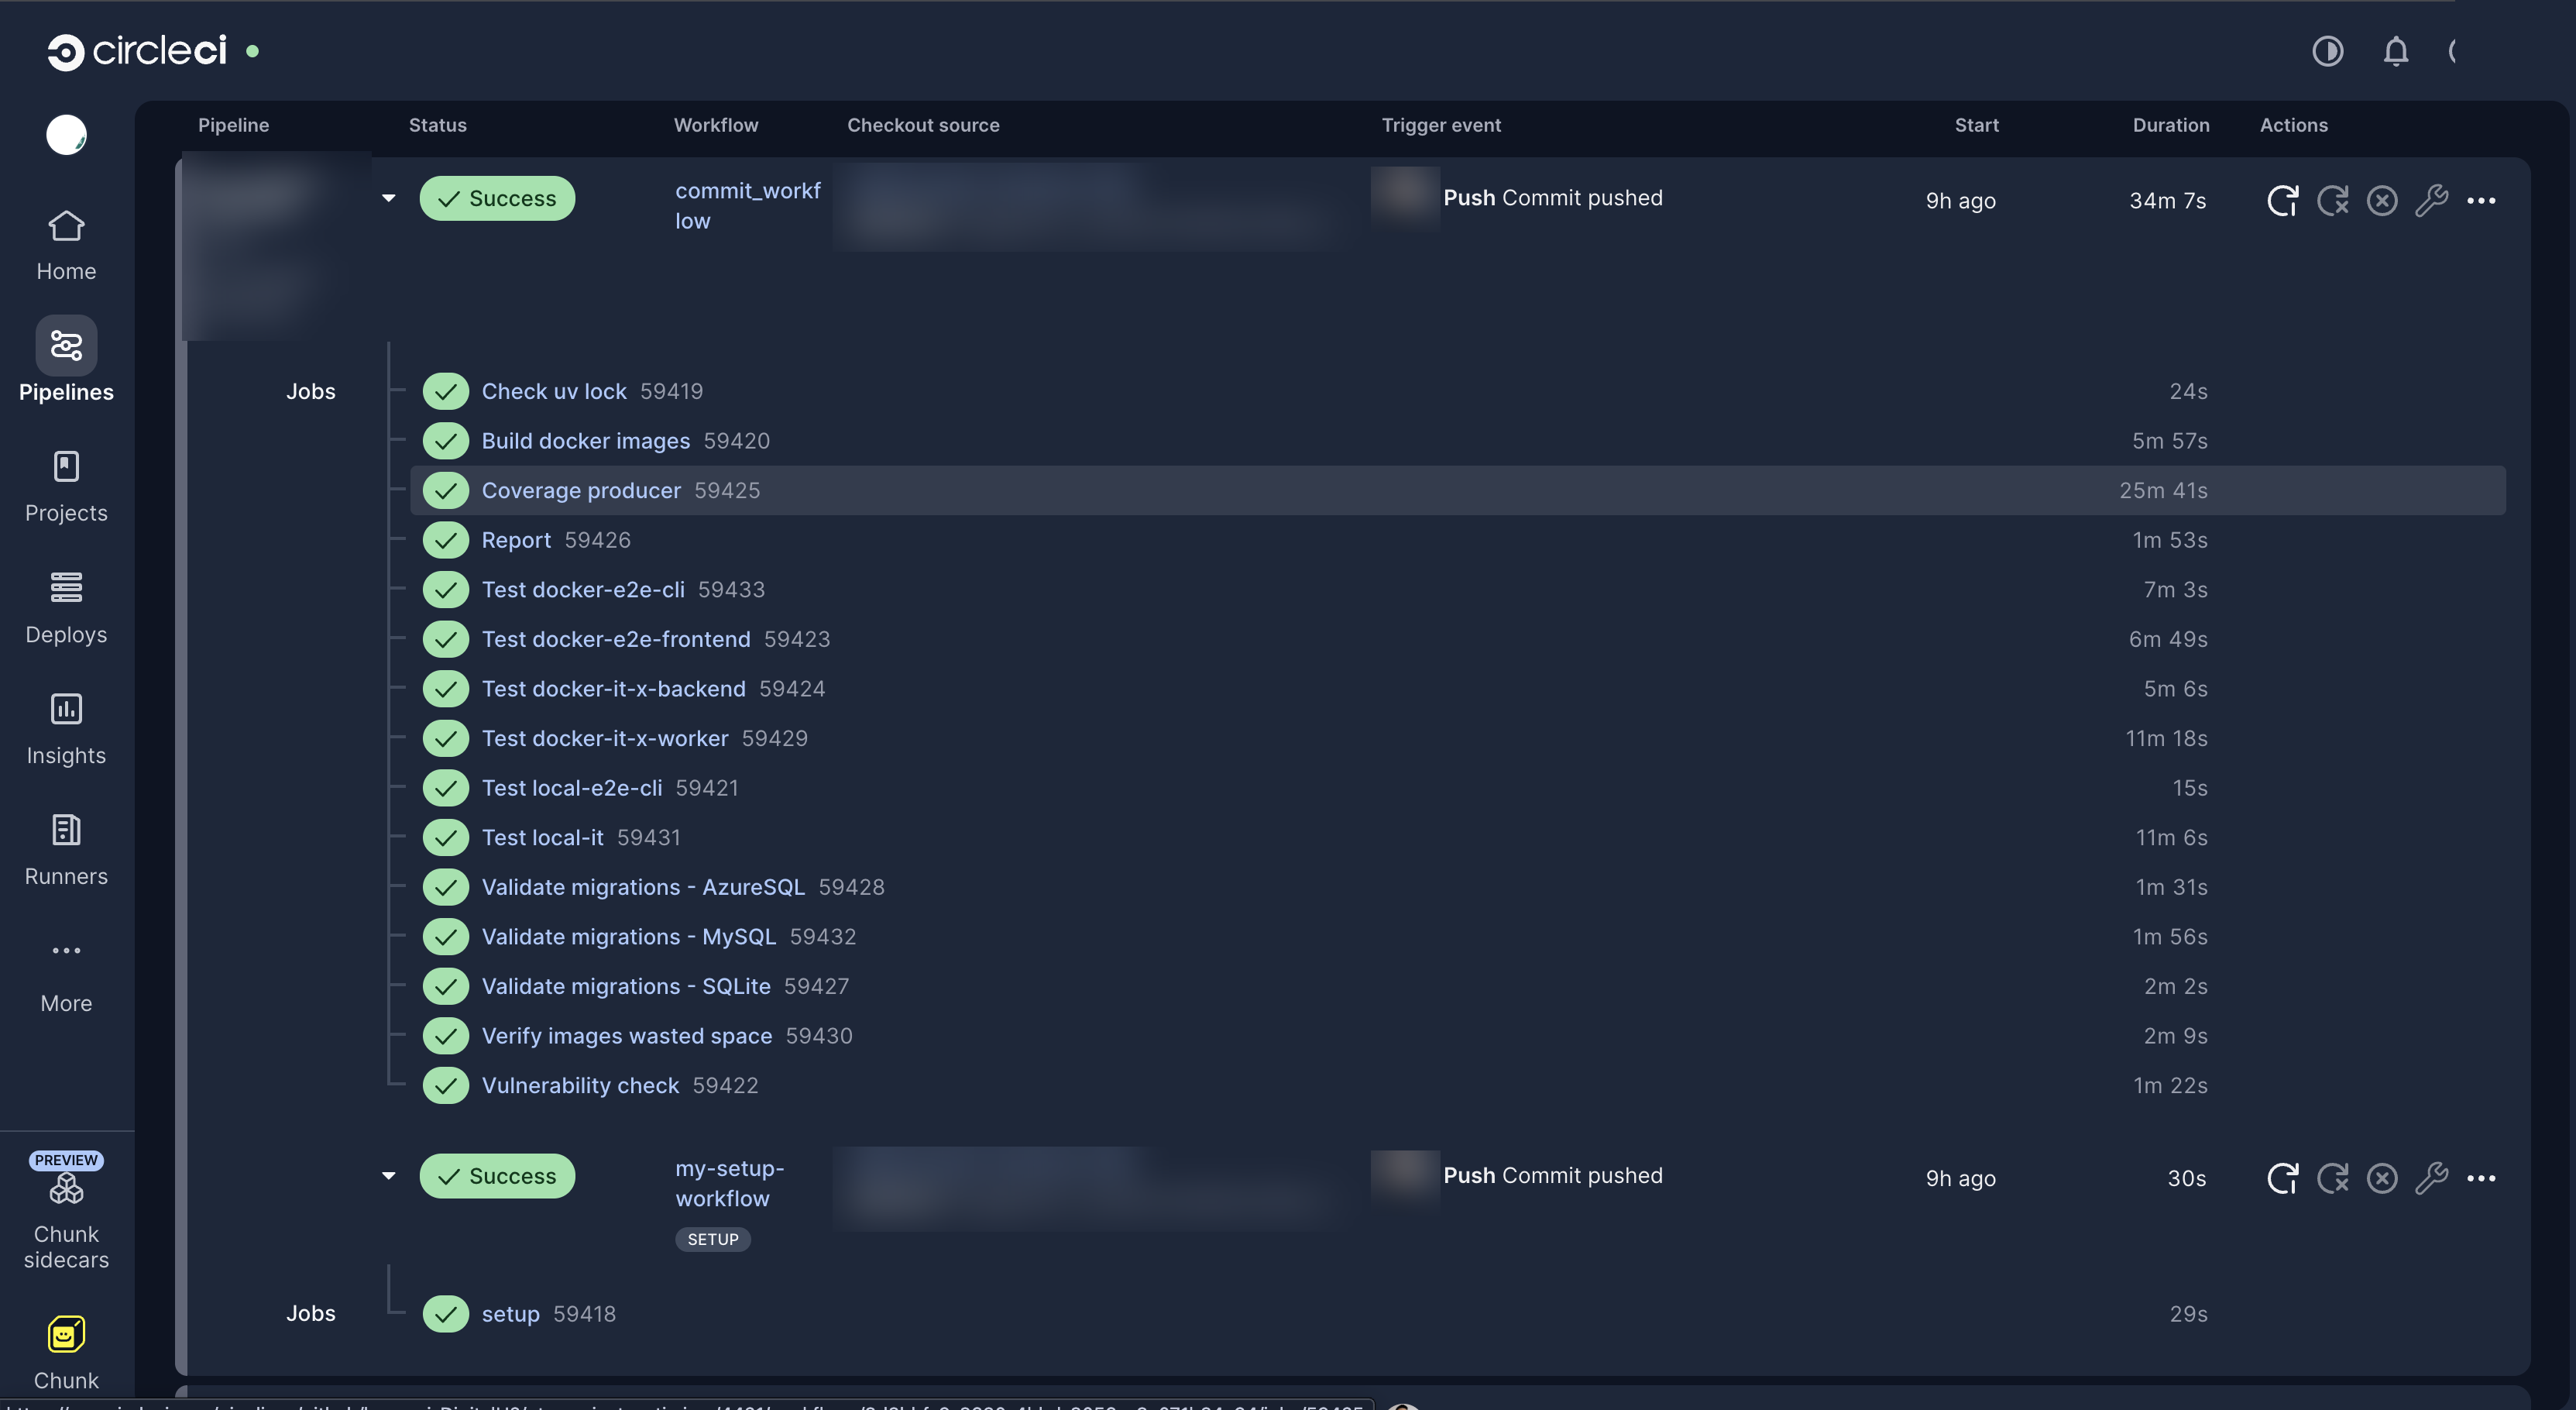
\includegraphics[width=0.95\linewidth]{Figures/chadi_circleci.png}
  \caption{CircleCI workflow: dependency checks, image builds, tests, migrations, and scans.}
  \label{fig:impl-circleci}
\end{figure}

\begin{figure}[H]
  \centering
  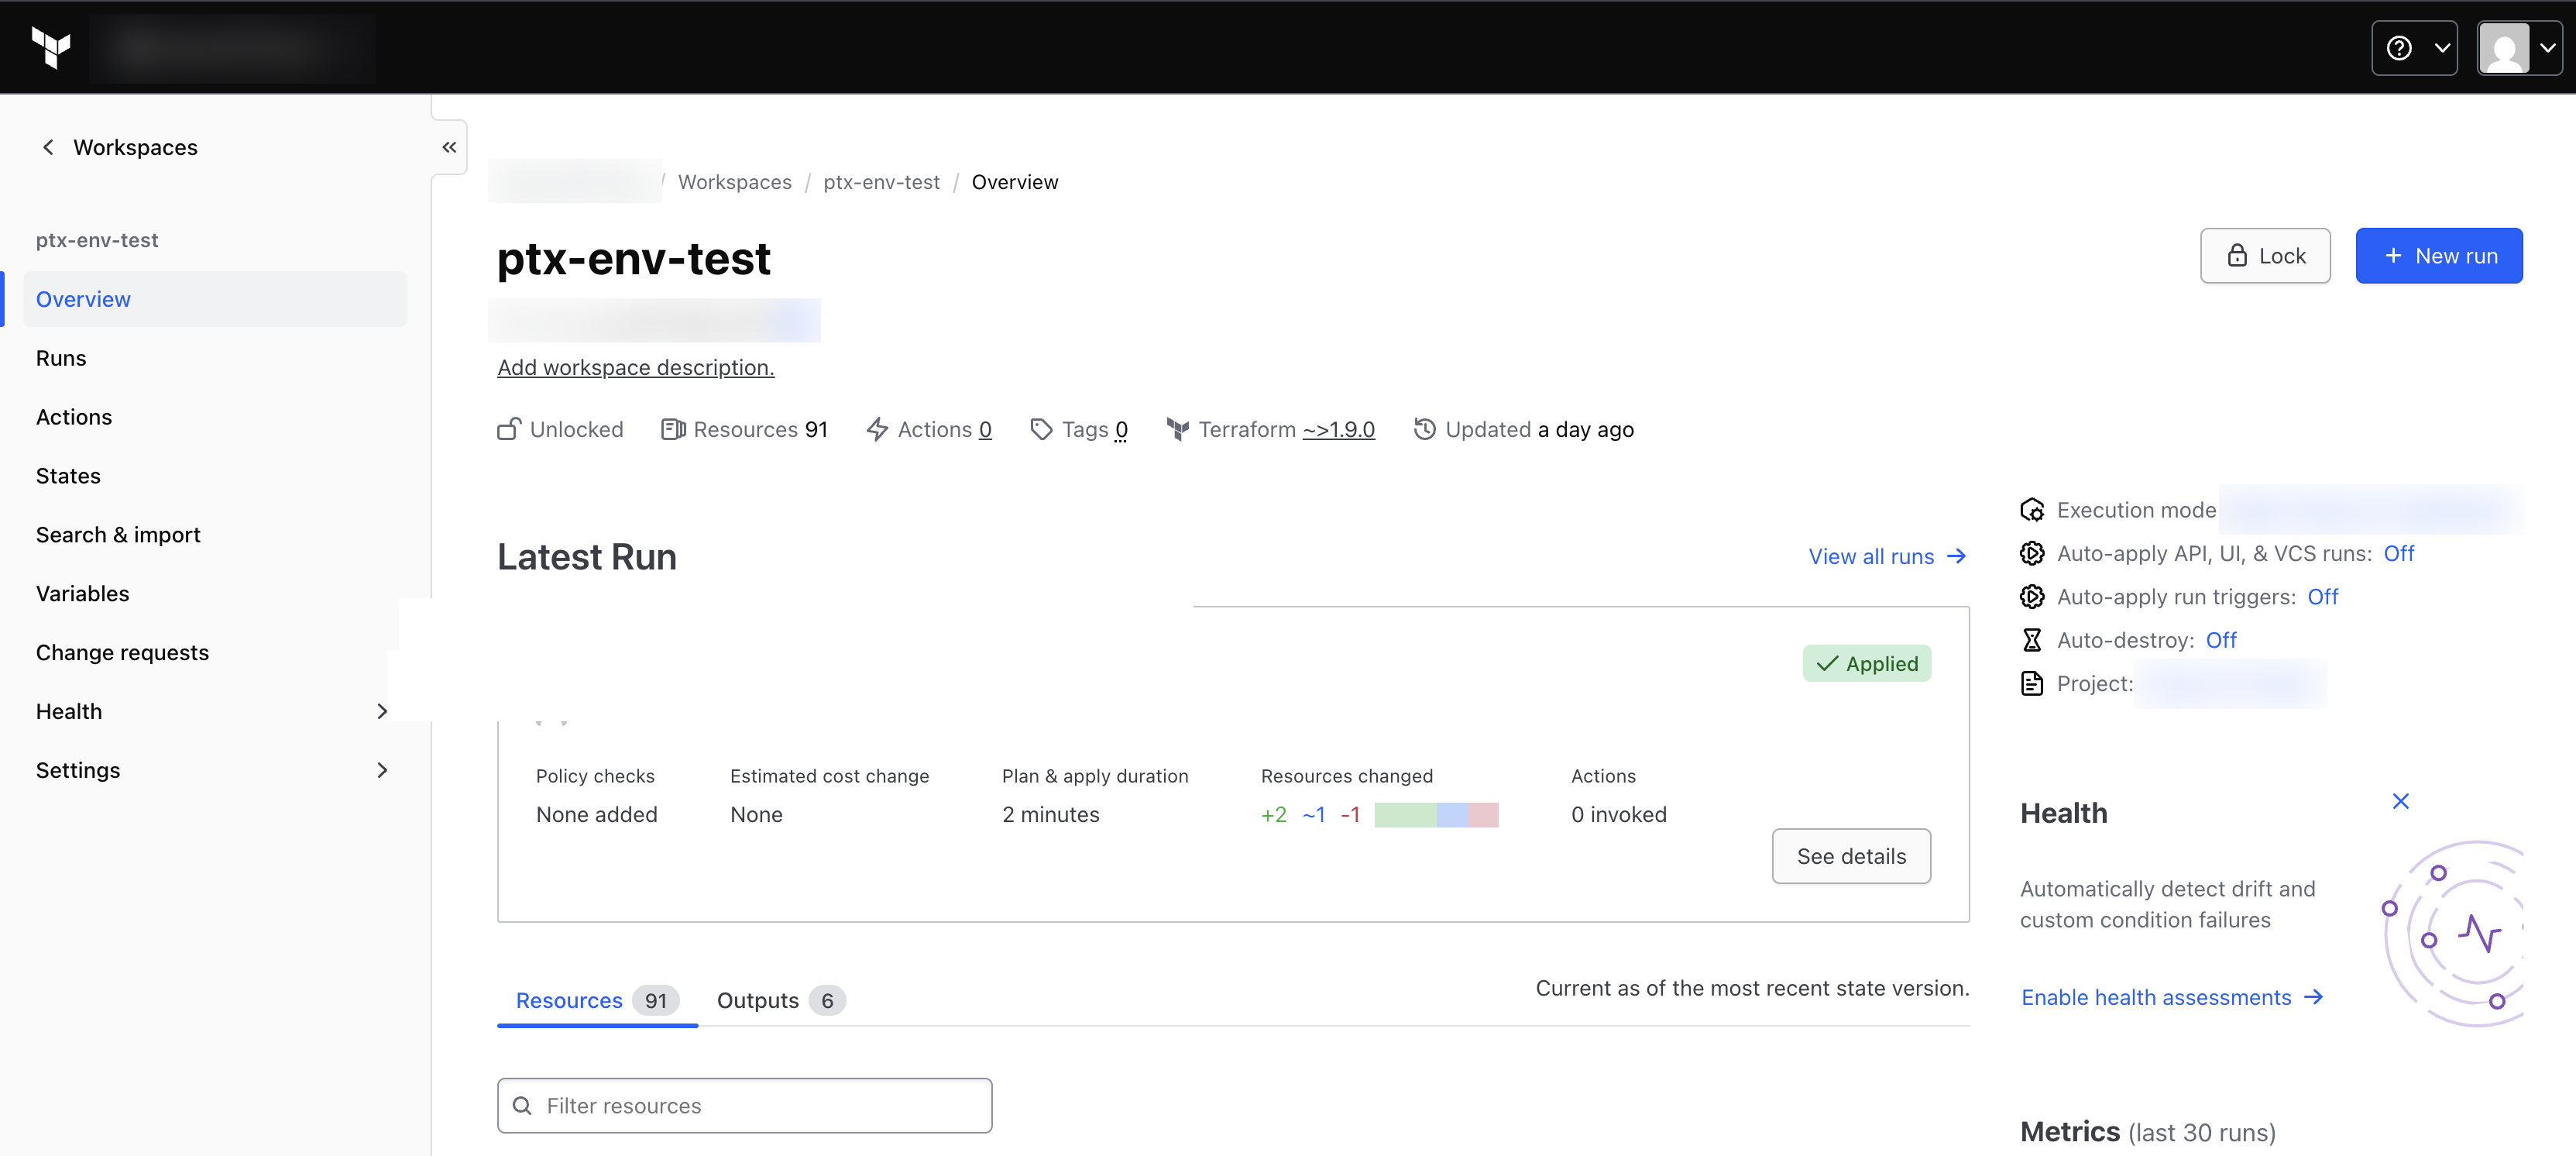
\includegraphics[width=0.95\linewidth]{Figures/chadi_terraform.png}
  \caption{Terraform run: infrastructure applied through a controlled workspace.}
  \label{fig:impl-terraform}
\end{figure}

\subsection{Operational QA and monitoring}

A scheduled monitoring loop assesses the health of the deployed system. It runs
deterministic checks first (public and internal reachability, read-only API checks,
and a synthetic end-to-end journey in a temporary test project) and then asks a
read-only assessment agent for an evidence-based status, summarized as GREEN,
YELLOW, or RED with suspected causes (Figure~\ref{fig:impl-qa}). The write actions
the loop needs (synthetic test setup and cleanup, report persistence, and
notifications) belong to the runner, not to the agent, which preserves the agent's
read-only contract while still surfacing severe findings.

\begin{figure}[H]
  \centering
  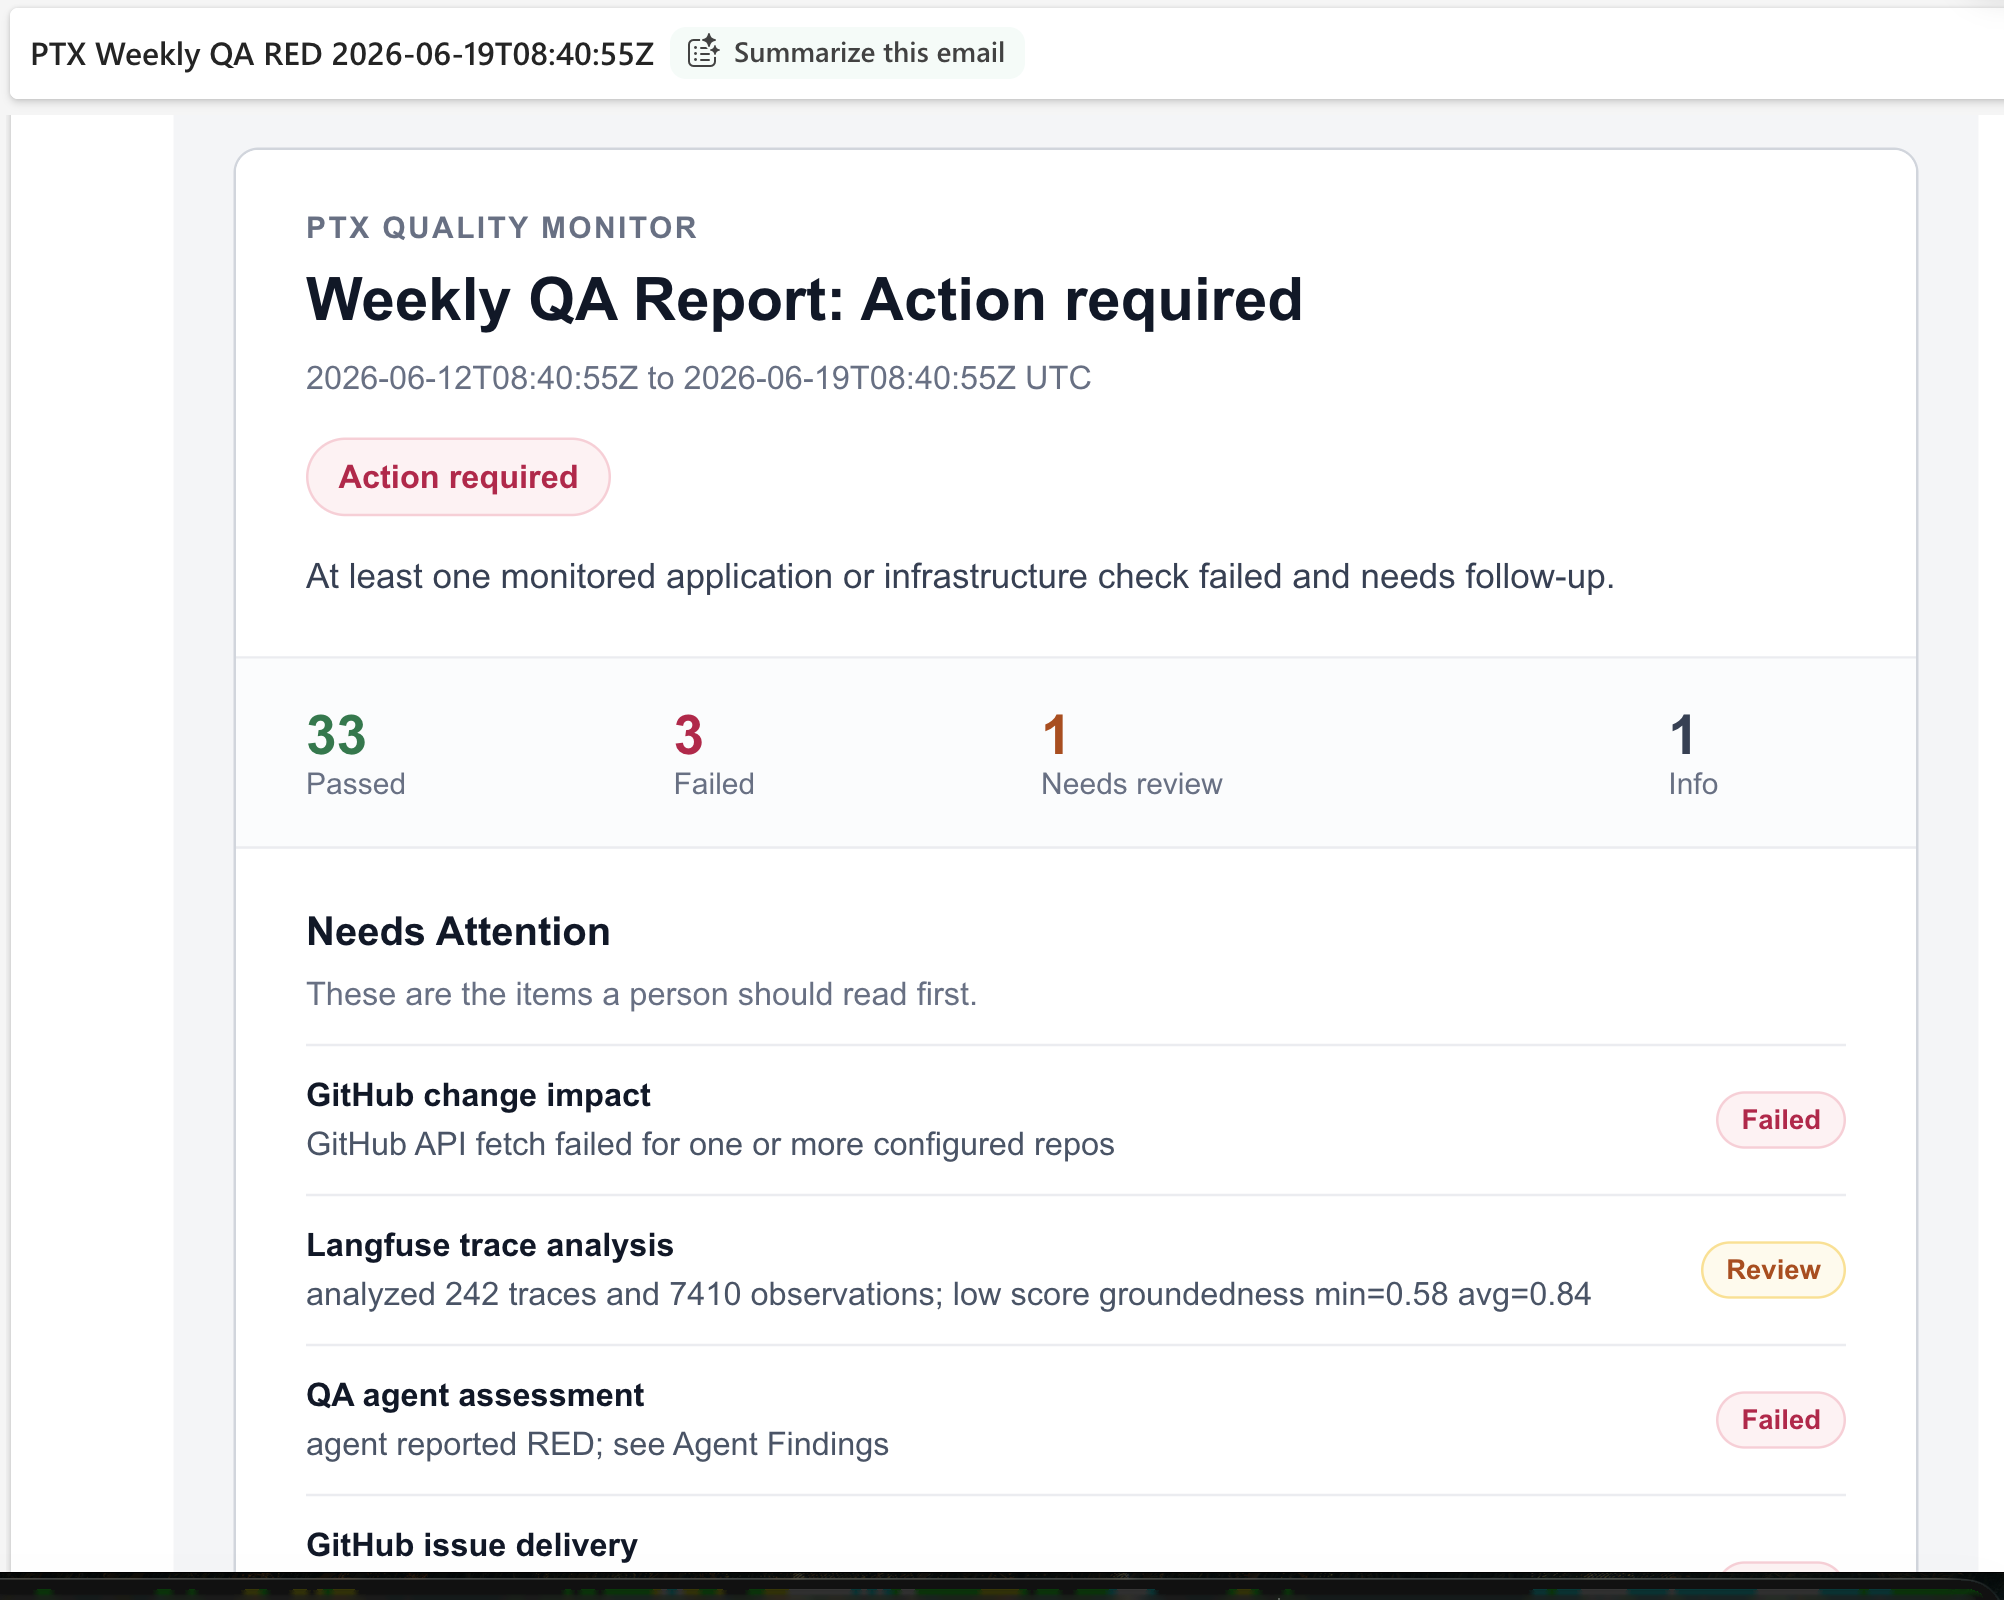
\includegraphics[width=0.62\linewidth]{Figures/chadi_qa_report.png}
  \caption{QA/SRE report: the weekly monitoring summary with items needing attention.}
  \label{fig:impl-qa}
\end{figure}

\subsection{Observability}

Assisted interactions are traced end-to-end in the observability platform, where
model calls, tool invocations, costs, evaluator scores, and prompt versions are
inspectable (Figures~\ref{fig:impl-langfuse} and~\ref{fig:impl-prompts}). This is
the evidence layer that lets a visible answer be traced back to the exact reasoning
and facts that produced it, and the same platform hosts the datasets and experiments
used by the evaluation harness.

\begin{figure}[H]
  \centering
  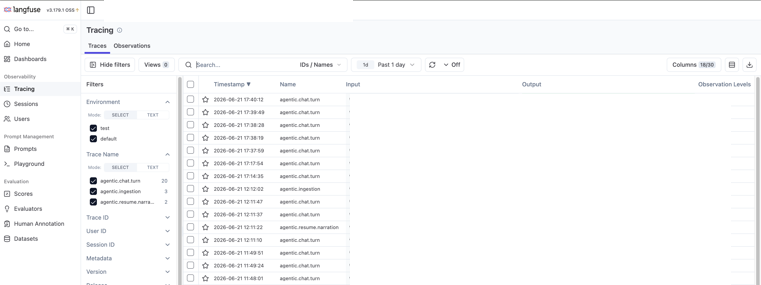
\includegraphics[width=\linewidth]{Figures/impl_langfuse.png}
  \caption{Langfuse traces: each assisted turn with its inputs, outputs, and levels.}
  \label{fig:impl-langfuse}
\end{figure}

\begin{figure}[H]
  \centering
  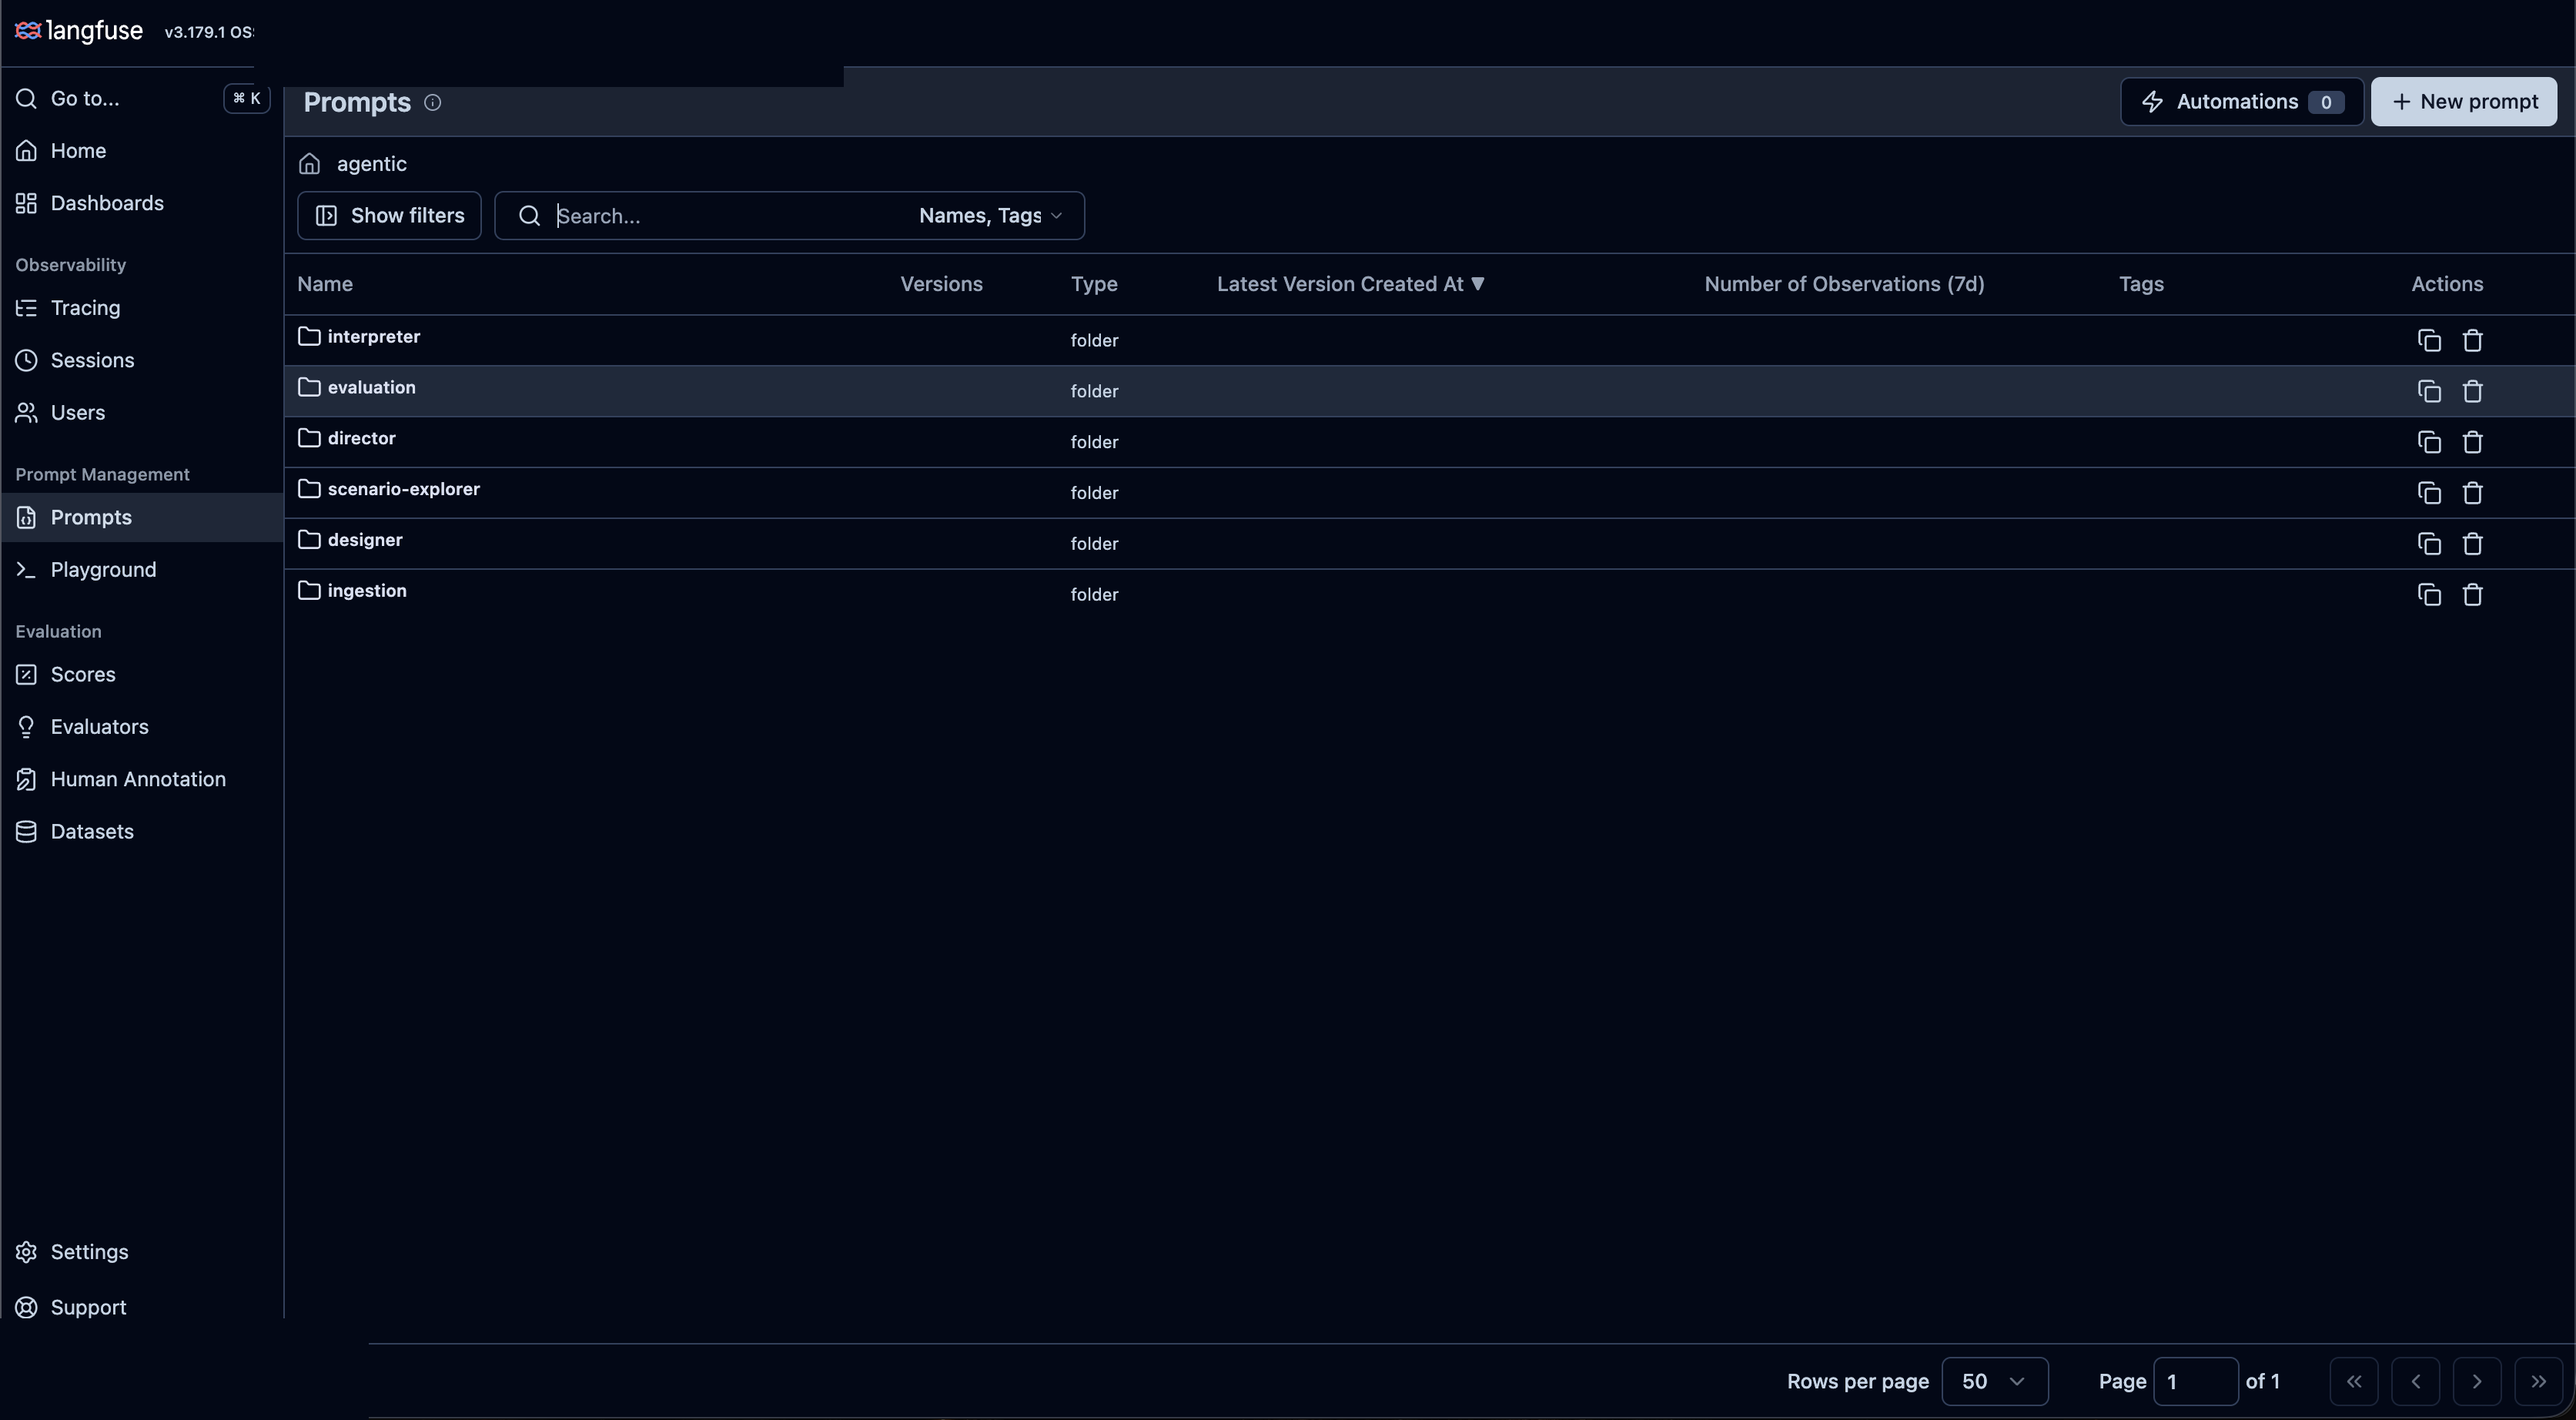
\includegraphics[width=0.9\linewidth]{Figures/chadi_prompt_registry.png}
  \caption{Prompt registry: versioned prompts for the Director and specialist agents.}
  \label{fig:impl-prompts}
\end{figure}

\section{Evaluation}
\label{sec:evaluation}

Because the assisted capabilities rely on a language model, they were measured
rather than assumed. Three complementary measurements are reported: the fidelity of
generated structures tracked across versions, the quality of the interpreter's
explanations scored by an independent judge, and the effort saved per stage of a
study. All are first-order results on a small sample, not a controlled study, and
the absolute figures should be read as order-of-magnitude evidence.\footnote{The
evaluation figures below are drawn from the project's own measurements and should
be confirmed against the final production runs.}

\subsection{Fidelity tracking and regression detection}

For structured outputs such as a generated topology, quality is measured against
curated golden references using a similarity derived from the graph edit distance
\cite{sanfeliu1983}, aggregated over a fixed golden set and compared against an
agreed acceptance threshold. Tracking this metric across versions turns evaluation
into a quantitative, repeatable signal. Figure~\ref{fig:ged} shows the value of the
harness: a change of the underlying model at version~4 silently degraded fidelity
below threshold, a regression that string- or eyeball-level checks would have
missed and that the metric caught before release, prompting a rollback at
version~5.

\begin{figure}[H]
  \centering
  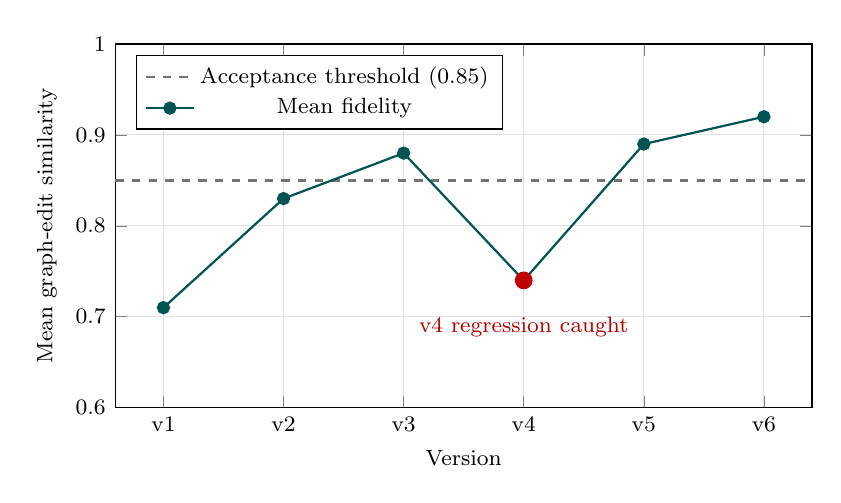
\begin{tikzpicture}
    \begin{axis}[
      width=0.86\linewidth, height=6.2cm,
      xlabel={Version}, ylabel={Mean graph-edit similarity},
      xmin=0.6, xmax=6.4, ymin=0.6, ymax=1.0,
      xtick={1,2,3,4,5,6}, xticklabels={v1,v2,v3,v4,v5,v6},
      ytick={0.6,0.7,0.8,0.9,1.0},
      grid=major, grid style={black!12},
      tick label style={font=\footnotesize}, label style={font=\footnotesize},
      legend style={font=\footnotesize, at={(0.03,0.97)}, anchor=north west},
      clip=false,
    ]
      \addplot[dashed, thick, black!55, samples=2, domain=0.6:6.4] {0.85};
      \addlegendentry{Acceptance threshold (0.85)}
      \addplot[mark=*, thick, teal!65!black] coordinates
        {(1,0.71) (2,0.83) (3,0.88) (4,0.74) (5,0.89) (6,0.92)};
      \addlegendentry{Mean fidelity}
      \addplot[only marks, mark=*, mark size=3pt, red!75!black] coordinates {(4,0.74)};
      \node[font=\footnotesize, red!70!black, anchor=north] at (axis cs:4,0.71)
        {v4 regression caught};
    \end{axis}
  \end{tikzpicture}
  \caption{Topology-designer fidelity across versions; the v4 model swap fell below threshold and was rolled back (illustrative).}
  \label{fig:ged}
\end{figure}

\subsection{Interpretation quality}

Interpretations, which are free text, are scored by an independent LLM-as-a-judge
on the four-dimension rubric of Section~\ref{sec:eval-design} (groundedness,
financial and commercial soundness, and operational coherence), each case scored
several times and aggregated \cite{zheng2023judge}. In the delivered system the same
judge runs in two modes. \textbf{Online}, it fires in the background after each
interpretation, sampled to control cost, and writes its four scores onto that turn's
trace, so quality is visible live (Figure~\ref{fig:impl-judge-scores}).
\textbf{Offline}, it runs over a curated dataset, so a change to the interpreter's
prompt is validated by comparing score deltas across versions as experiments in the
observability platform \cite{langfuse2025}. User thumbs feedback is recorded as
scores and promotes weak turns into the dataset, which closes the loop between
production use and the next round of prompt work. The evaluation is therefore
reproducible on a fixed dataset and tied to explicit dimensions, so a change in
interpretation quality surfaces as a score delta across versions rather than as an
anecdote.

\begin{figure}[H]
  \centering
  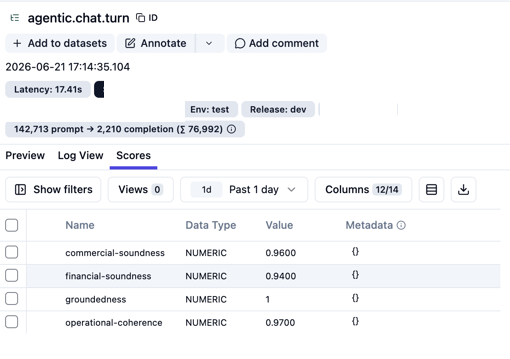
\includegraphics[width=0.72\linewidth]{Figures/impl_judge.png}
  \caption{Automatic evaluation: four judge dimensions on an interpretation's trace (header figures are for the enclosing chat turn).}
  \label{fig:impl-judge-scores}
\end{figure}

\subsection{Impact on analyst effort}

The agentic layer was also assessed against the manual baseline it assists. Each
stage of a study was decomposed into its constituent steps, the manual baseline was
taken from the time practitioners spend today, and the assisted figure was measured
end-to-end with the expert kept in the loop. Figure~\ref{fig:effort} contrasts the
two. The headline for this contribution is the last group: the interpretation of
results, previously a manual expert task, becomes a short grounded conversation.

\begin{figure}[H]
  \centering
  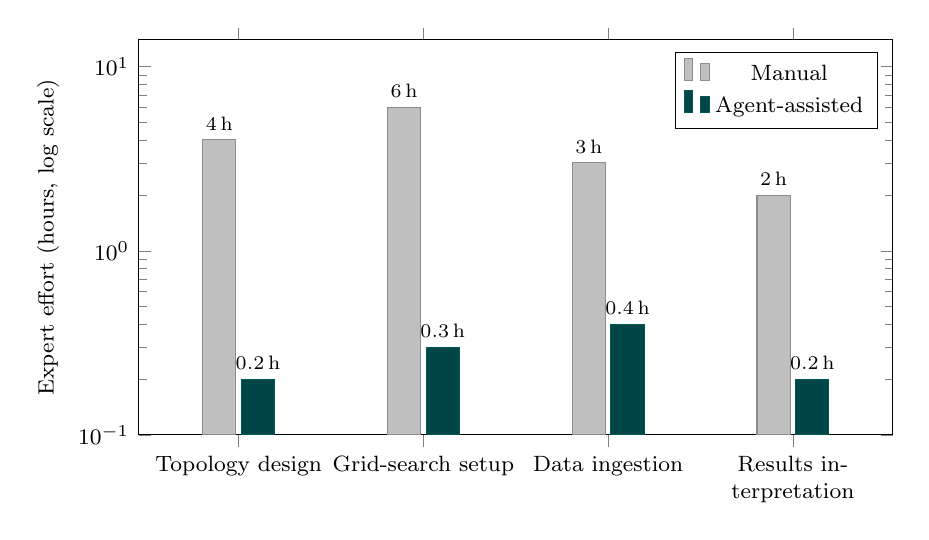
\begin{tikzpicture}
    \begin{axis}[
      ybar, width=0.92\linewidth, height=6.6cm,
      ymode=log, ymin=0.1, ymax=14, log origin=infty,
      ylabel={Expert effort (hours, log scale)},
      symbolic x coords={Topology design, Grid-search setup, Data ingestion,
        Results interpretation},
      xtick=data,
      x tick label style={font=\footnotesize, align=center, text width=2.5cm},
      tick label style={font=\footnotesize}, label style={font=\footnotesize},
      bar width=12pt, enlarge x limits=0.18,
      legend style={font=\footnotesize, at={(0.98,0.97)}, anchor=north east},
      point meta=rawy,
      nodes near coords={\pgfmathprintnumber{\pgfplotspointmeta}\,h},
      every node near coord/.append style={font=\scriptsize, anchor=south},
    ]
      \addplot[fill=black!25, draw=black!45] coordinates
        {(Topology design,4) (Grid-search setup,6) (Data ingestion,3)
         (Results interpretation,2)};
      \addplot[fill=teal!55!black, draw=teal!70!black] coordinates
        {(Topology design,0.2) (Grid-search setup,0.3) (Data ingestion,0.4)
         (Results interpretation,0.2)};
      \legend{Manual, Agent-assisted}
    \end{axis}
  \end{tikzpicture}
  \caption{Expert effort per stage, manual versus agent-assisted (log scale; representative order-of-magnitude estimates).}
  \label{fig:effort}
\end{figure}

Beyond raw time, and arguably more defensible than any single figure, the work
improves \emph{consistency} (every interpretation follows the same grounded
rubric), \emph{traceability} (every figure is linked to a deterministic result),
and \emph{accessibility} (a non-specialist can obtain and audit an interpretation
on the cases evaluated), the qualities that ultimately widen the set of people who
can use the tool.

\section*{Conclusion}

This chapter presented the concrete implementation of the restored and extended
Energy Transition Optimizer. It identified the main technologies across the
frontend, backend, deterministic execution, agentic layer, persistence, cloud
runtime, identity, and delivery; documented the
implemented product through the showcase, from product entry and the deterministic
workspace to agentic creation, ingestion, topology generation, and result
exploration and interpretation; and reported the
platform and operations work around enterprise access, automated delivery,
infrastructure-as-code, QA monitoring, and observability. It closed with the
evaluation: a fidelity metric that catches regressions, an LLM-as-a-judge scoring
of interpretations, and an order-of-magnitude reduction in the effort required to
interpret results. Deterministic computation remains the source of numerical truth,
assisted workflows remain approval-gated, and platform operation is supported by
repeatable deployment and observable runtime behavior. The general conclusion now
summarizes the outcomes of the internship and its broader perspectives.
